% Options for packages loaded elsewhere
\PassOptionsToPackage{unicode}{hyperref}
\PassOptionsToPackage{hyphens}{url}
\PassOptionsToPackage{dvipsnames,svgnames,x11names}{xcolor}
%
\documentclass[
  letterpaper,
  DIV=11,
  numbers=noendperiod]{scrreprt}

\usepackage{amsmath,amssymb}
\usepackage{iftex}
\ifPDFTeX
  \usepackage[T1]{fontenc}
  \usepackage[utf8]{inputenc}
  \usepackage{textcomp} % provide euro and other symbols
\else % if luatex or xetex
  \usepackage{unicode-math}
  \defaultfontfeatures{Scale=MatchLowercase}
  \defaultfontfeatures[\rmfamily]{Ligatures=TeX,Scale=1}
\fi
\usepackage{lmodern}
\ifPDFTeX\else  
    % xetex/luatex font selection
\fi
% Use upquote if available, for straight quotes in verbatim environments
\IfFileExists{upquote.sty}{\usepackage{upquote}}{}
\IfFileExists{microtype.sty}{% use microtype if available
  \usepackage[]{microtype}
  \UseMicrotypeSet[protrusion]{basicmath} % disable protrusion for tt fonts
}{}
\makeatletter
\@ifundefined{KOMAClassName}{% if non-KOMA class
  \IfFileExists{parskip.sty}{%
    \usepackage{parskip}
  }{% else
    \setlength{\parindent}{0pt}
    \setlength{\parskip}{6pt plus 2pt minus 1pt}}
}{% if KOMA class
  \KOMAoptions{parskip=half}}
\makeatother
\usepackage{xcolor}
\setlength{\emergencystretch}{3em} % prevent overfull lines
\setcounter{secnumdepth}{1}
% Make \paragraph and \subparagraph free-standing
\ifx\paragraph\undefined\else
  \let\oldparagraph\paragraph
  \renewcommand{\paragraph}[1]{\oldparagraph{#1}\mbox{}}
\fi
\ifx\subparagraph\undefined\else
  \let\oldsubparagraph\subparagraph
  \renewcommand{\subparagraph}[1]{\oldsubparagraph{#1}\mbox{}}
\fi

\usepackage{color}
\usepackage{fancyvrb}
\newcommand{\VerbBar}{|}
\newcommand{\VERB}{\Verb[commandchars=\\\{\}]}
\DefineVerbatimEnvironment{Highlighting}{Verbatim}{commandchars=\\\{\}}
% Add ',fontsize=\small' for more characters per line
\usepackage{framed}
\definecolor{shadecolor}{RGB}{241,243,245}
\newenvironment{Shaded}{\begin{snugshade}}{\end{snugshade}}
\newcommand{\AlertTok}[1]{\textcolor[rgb]{0.68,0.00,0.00}{#1}}
\newcommand{\AnnotationTok}[1]{\textcolor[rgb]{0.37,0.37,0.37}{#1}}
\newcommand{\AttributeTok}[1]{\textcolor[rgb]{0.40,0.45,0.13}{#1}}
\newcommand{\BaseNTok}[1]{\textcolor[rgb]{0.68,0.00,0.00}{#1}}
\newcommand{\BuiltInTok}[1]{\textcolor[rgb]{0.00,0.23,0.31}{#1}}
\newcommand{\CharTok}[1]{\textcolor[rgb]{0.13,0.47,0.30}{#1}}
\newcommand{\CommentTok}[1]{\textcolor[rgb]{0.37,0.37,0.37}{#1}}
\newcommand{\CommentVarTok}[1]{\textcolor[rgb]{0.37,0.37,0.37}{\textit{#1}}}
\newcommand{\ConstantTok}[1]{\textcolor[rgb]{0.56,0.35,0.01}{#1}}
\newcommand{\ControlFlowTok}[1]{\textcolor[rgb]{0.00,0.23,0.31}{#1}}
\newcommand{\DataTypeTok}[1]{\textcolor[rgb]{0.68,0.00,0.00}{#1}}
\newcommand{\DecValTok}[1]{\textcolor[rgb]{0.68,0.00,0.00}{#1}}
\newcommand{\DocumentationTok}[1]{\textcolor[rgb]{0.37,0.37,0.37}{\textit{#1}}}
\newcommand{\ErrorTok}[1]{\textcolor[rgb]{0.68,0.00,0.00}{#1}}
\newcommand{\ExtensionTok}[1]{\textcolor[rgb]{0.00,0.23,0.31}{#1}}
\newcommand{\FloatTok}[1]{\textcolor[rgb]{0.68,0.00,0.00}{#1}}
\newcommand{\FunctionTok}[1]{\textcolor[rgb]{0.28,0.35,0.67}{#1}}
\newcommand{\ImportTok}[1]{\textcolor[rgb]{0.00,0.46,0.62}{#1}}
\newcommand{\InformationTok}[1]{\textcolor[rgb]{0.37,0.37,0.37}{#1}}
\newcommand{\KeywordTok}[1]{\textcolor[rgb]{0.00,0.23,0.31}{#1}}
\newcommand{\NormalTok}[1]{\textcolor[rgb]{0.00,0.23,0.31}{#1}}
\newcommand{\OperatorTok}[1]{\textcolor[rgb]{0.37,0.37,0.37}{#1}}
\newcommand{\OtherTok}[1]{\textcolor[rgb]{0.00,0.23,0.31}{#1}}
\newcommand{\PreprocessorTok}[1]{\textcolor[rgb]{0.68,0.00,0.00}{#1}}
\newcommand{\RegionMarkerTok}[1]{\textcolor[rgb]{0.00,0.23,0.31}{#1}}
\newcommand{\SpecialCharTok}[1]{\textcolor[rgb]{0.37,0.37,0.37}{#1}}
\newcommand{\SpecialStringTok}[1]{\textcolor[rgb]{0.13,0.47,0.30}{#1}}
\newcommand{\StringTok}[1]{\textcolor[rgb]{0.13,0.47,0.30}{#1}}
\newcommand{\VariableTok}[1]{\textcolor[rgb]{0.07,0.07,0.07}{#1}}
\newcommand{\VerbatimStringTok}[1]{\textcolor[rgb]{0.13,0.47,0.30}{#1}}
\newcommand{\WarningTok}[1]{\textcolor[rgb]{0.37,0.37,0.37}{\textit{#1}}}

\providecommand{\tightlist}{%
  \setlength{\itemsep}{0pt}\setlength{\parskip}{0pt}}\usepackage{longtable,booktabs,array}
\usepackage{calc} % for calculating minipage widths
% Correct order of tables after \paragraph or \subparagraph
\usepackage{etoolbox}
\makeatletter
\patchcmd\longtable{\par}{\if@noskipsec\mbox{}\fi\par}{}{}
\makeatother
% Allow footnotes in longtable head/foot
\IfFileExists{footnotehyper.sty}{\usepackage{footnotehyper}}{\usepackage{footnote}}
\makesavenoteenv{longtable}
\usepackage{graphicx}
\makeatletter
\def\maxwidth{\ifdim\Gin@nat@width>\linewidth\linewidth\else\Gin@nat@width\fi}
\def\maxheight{\ifdim\Gin@nat@height>\textheight\textheight\else\Gin@nat@height\fi}
\makeatother
% Scale images if necessary, so that they will not overflow the page
% margins by default, and it is still possible to overwrite the defaults
% using explicit options in \includegraphics[width, height, ...]{}
\setkeys{Gin}{width=\maxwidth,height=\maxheight,keepaspectratio}
% Set default figure placement to htbp
\makeatletter
\def\fps@figure{htbp}
\makeatother
\newlength{\cslhangindent}
\setlength{\cslhangindent}{1.5em}
\newlength{\csllabelwidth}
\setlength{\csllabelwidth}{3em}
\newlength{\cslentryspacingunit} % times entry-spacing
\setlength{\cslentryspacingunit}{\parskip}
\newenvironment{CSLReferences}[2] % #1 hanging-ident, #2 entry spacing
 {% don't indent paragraphs
  \setlength{\parindent}{0pt}
  % turn on hanging indent if param 1 is 1
  \ifodd #1
  \let\oldpar\par
  \def\par{\hangindent=\cslhangindent\oldpar}
  \fi
  % set entry spacing
  \setlength{\parskip}{#2\cslentryspacingunit}
 }%
 {}
\usepackage{calc}
\newcommand{\CSLBlock}[1]{#1\hfill\break}
\newcommand{\CSLLeftMargin}[1]{\parbox[t]{\csllabelwidth}{#1}}
\newcommand{\CSLRightInline}[1]{\parbox[t]{\linewidth - \csllabelwidth}{#1}\break}
\newcommand{\CSLIndent}[1]{\hspace{\cslhangindent}#1}

\usepackage{makeidx}
\makeindex
\KOMAoption{captions}{tableheading}
\makeatletter
\@ifpackageloaded{tcolorbox}{}{\usepackage[skins,breakable]{tcolorbox}}
\@ifpackageloaded{fontawesome5}{}{\usepackage{fontawesome5}}
\definecolor{quarto-callout-color}{HTML}{909090}
\definecolor{quarto-callout-note-color}{HTML}{0758E5}
\definecolor{quarto-callout-important-color}{HTML}{CC1914}
\definecolor{quarto-callout-warning-color}{HTML}{EB9113}
\definecolor{quarto-callout-tip-color}{HTML}{00A047}
\definecolor{quarto-callout-caution-color}{HTML}{FC5300}
\definecolor{quarto-callout-color-frame}{HTML}{acacac}
\definecolor{quarto-callout-note-color-frame}{HTML}{4582ec}
\definecolor{quarto-callout-important-color-frame}{HTML}{d9534f}
\definecolor{quarto-callout-warning-color-frame}{HTML}{f0ad4e}
\definecolor{quarto-callout-tip-color-frame}{HTML}{02b875}
\definecolor{quarto-callout-caution-color-frame}{HTML}{fd7e14}
\makeatother
\makeatletter
\makeatother
\makeatletter
\@ifpackageloaded{bookmark}{}{\usepackage{bookmark}}
\makeatother
\makeatletter
\@ifpackageloaded{caption}{}{\usepackage{caption}}
\AtBeginDocument{%
\ifdefined\contentsname
  \renewcommand*\contentsname{Table of contents}
\else
  \newcommand\contentsname{Table of contents}
\fi
\ifdefined\listfigurename
  \renewcommand*\listfigurename{List of Figures}
\else
  \newcommand\listfigurename{List of Figures}
\fi
\ifdefined\listtablename
  \renewcommand*\listtablename{List of Tables}
\else
  \newcommand\listtablename{List of Tables}
\fi
\ifdefined\figurename
  \renewcommand*\figurename{Figure}
\else
  \newcommand\figurename{Figure}
\fi
\ifdefined\tablename
  \renewcommand*\tablename{Table}
\else
  \newcommand\tablename{Table}
\fi
}
\@ifpackageloaded{float}{}{\usepackage{float}}
\floatstyle{ruled}
\@ifundefined{c@chapter}{\newfloat{codelisting}{h}{lop}}{\newfloat{codelisting}{h}{lop}[chapter]}
\floatname{codelisting}{Listing}
\newcommand*\listoflistings{\listof{codelisting}{List of Listings}}
\makeatother
\makeatletter
\@ifpackageloaded{caption}{}{\usepackage{caption}}
\@ifpackageloaded{subcaption}{}{\usepackage{subcaption}}
\makeatother
\makeatletter
\@ifpackageloaded{tcolorbox}{}{\usepackage[skins,breakable]{tcolorbox}}
\makeatother
\makeatletter
\@ifundefined{shadecolor}{\definecolor{shadecolor}{rgb}{.97, .97, .97}}
\makeatother
\makeatletter
\makeatother
\makeatletter
\makeatother
\ifLuaTeX
  \usepackage{selnolig}  % disable illegal ligatures
\fi
\IfFileExists{bookmark.sty}{\usepackage{bookmark}}{\usepackage{hyperref}}
\IfFileExists{xurl.sty}{\usepackage{xurl}}{} % add URL line breaks if available
\urlstyle{same} % disable monospaced font for URLs
\hypersetup{
  pdftitle={Cresko Laboratory Procedures and Protocols},
  pdfauthor={Cresko Laboratory},
  colorlinks=true,
  linkcolor={blue},
  filecolor={Maroon},
  citecolor={Blue},
  urlcolor={Blue},
  pdfcreator={LaTeX via pandoc}}

\title{Cresko Laboratory Procedures and Protocols}
\author{Cresko Laboratory}
\date{Friday, March 1, 2024}

\begin{document}
\maketitle
\ifdefined\Shaded\renewenvironment{Shaded}{\begin{tcolorbox}[enhanced, boxrule=0pt, sharp corners, frame hidden, interior hidden, borderline west={3pt}{0pt}{shadecolor}, breakable]}{\end{tcolorbox}}\fi

\renewcommand*\contentsname{Table of contents}
{
\hypersetup{linkcolor=}
\setcounter{tocdepth}{2}
\tableofcontents
}
\bookmarksetup{startatroot}

\hypertarget{how-to-use-this-book}{%
\chapter*{How to use this book}\label{how-to-use-this-book}}
\addcontentsline{toc}{chapter}{How to use this book}

\markboth{How to use this book}{How to use this book}

This is a Quarto book that contains all of the Procedures and Protocols
for the Cresko Laboratory in the Institute of Ecology and Evolution at
the University of Oregon.

The book is organized into major section that contain

\begin{itemize}
\item
  General Laboratory Protocols or the lab
\item
  More detailed Laboratory Protocols
\item
  Husbandry protocols for vertebrate animals primarily stickleback and
  pipefish, but also zebrafish
\item
  Husbandry protocols for \emph{Daphnia}
\item
  Bioinformatic protocols including how to get on to \textbf{Talapas}
\end{itemize}

You can scroll through the book using the index on the left, but also
use the search field to find all relevant protocols.

There are also useful appendices at the end, as well as a section for
the references cited throughout the book.

This book was written in Markdown using Quarto. To learn more about
Quarto books visit \url{https://quarto.org/docs/books}.

\part{General Laboratory Protocols}

This section of the book contains general protocols for working in the
laboratory.

\hypertarget{sec-general-contact}{%
\chapter{Contact Information}\label{sec-general-contact}}

\begin{longtable}[]{@{}lll@{}}
\toprule\noalign{}
Col1 & Col2 & Col3 \\
\midrule\noalign{}
\endhead
\bottomrule\noalign{}
\endlastfoot
Bill Cresko & 541-285-5446 & Cell \\
Mark Currey & 541-505-0006 & Cell \\
Susie Bassham & xxxx & Cell \\
\end{longtable}

\part{Molecular Protocols}

This section of the book contains common protocols used for molecular
biology and genomics in the laboratory. These include standard protocols
such as setting up creating reagents, setting up PCRs and running gels,
as well as advanced protocols such as creating constructs.

\hypertarget{sec-molec-Phusion_PCR}{%
\chapter{PCR with Phusion}\label{sec-molec-Phusion_PCR}}

\hypertarget{introduction}{%
\section{Introduction}\label{introduction}}

\begin{itemize}
\tightlist
\item
  \textbf{Purpose}: This procedure describes how to set up a basic PCR
  with Phusion polymerase
\item
  \textbf{Procedure Type}: Molecular
\item
  \textbf{Species}: N/A
\end{itemize}

The following guidelines are provided to ensure successful PCR using
Phusion®~DNA Polymerase. These guidelines cover routine PCR.
Amplification of templates with high GC content, high secondary
structure, low template concentrations or long amplicons may require
further optimization.

We recommend assembling all reaction components on ice and quickly
transferring the reactions to a thermocycler preheated to the
denaturation temperature (98°C). All components should be mixed and
centrifuged prior to use. It is important to add Phusion DNA Polymerase
last in order to prevent any primer degradation caused by the 3´→ 5´
exonuclease activity.

Phusion DNA Polymerase may be diluted in 1X HF or GC Buffer just prior
to use in order to reduce pipetting errors. Please note that protocols
with Phusion DNA Polymerase may differ from protocols with other
standard polymerases. As such, conditions recommended below should be
used for optimal performance.

\hypertarget{materials}{%
\section{Materials:}\label{materials}}

\begin{itemize}
\tightlist
\item
  PCR tubes, plates or strip tubes (1 per reaction \& 1 for positive
  control)
\item
  Forward and reverse primers
\item
  npH2O
\item
  Phusion DNA polymerase
\item
  5X Phusion HF or GC Buffer
\item
  10 mM dNTPs
\item
  DMSo (optional)
\end{itemize}

\hypertarget{solutions}{%
\section{Solutions:}\label{solutions}}

NONE

\hypertarget{procedure}{%
\section{Procedure:}\label{procedure}}

\hypertarget{prepare-pcr-reactions}{%
\subsection{Prepare PCR reactions}\label{prepare-pcr-reactions}}

\begin{longtable}[]{@{}
  >{\raggedright\arraybackslash}p{(\columnwidth - 8\tabcolsep) * \real{0.0633}}
  >{\raggedright\arraybackslash}p{(\columnwidth - 8\tabcolsep) * \real{0.2785}}
  >{\raggedright\arraybackslash}p{(\columnwidth - 8\tabcolsep) * \real{0.1899}}
  >{\raggedright\arraybackslash}p{(\columnwidth - 8\tabcolsep) * \real{0.1899}}
  >{\raggedright\arraybackslash}p{(\columnwidth - 8\tabcolsep) * \real{0.2785}}@{}}
\caption{Table 1. Mixtures for PCR Reaction}\tabularnewline
\toprule\noalign{}
\begin{minipage}[b]{\linewidth}\raggedright
\end{minipage} & \begin{minipage}[b]{\linewidth}\raggedright
Component
\end{minipage} & \begin{minipage}[b]{\linewidth}\raggedright
20ul Reaction
\end{minipage} & \begin{minipage}[b]{\linewidth}\raggedright
50ul Reaction
\end{minipage} & \begin{minipage}[b]{\linewidth}\raggedright
Final Concentration
\end{minipage} \\
\midrule\noalign{}
\endfirsthead
\toprule\noalign{}
\begin{minipage}[b]{\linewidth}\raggedright
\end{minipage} & \begin{minipage}[b]{\linewidth}\raggedright
Component
\end{minipage} & \begin{minipage}[b]{\linewidth}\raggedright
20ul Reaction
\end{minipage} & \begin{minipage}[b]{\linewidth}\raggedright
50ul Reaction
\end{minipage} & \begin{minipage}[b]{\linewidth}\raggedright
Final Concentration
\end{minipage} \\
\midrule\noalign{}
\endhead
\bottomrule\noalign{}
\endlastfoot
1 & npH20 & to 20 ul & to 50 ul & \\
2 & 5x Phusion Buffer & 4 ul & 10 ul & 1X \\
3 & 10mM dNTPs & 0.4ul & 1.0 ul & 200 uM \\
4 & 10 uM forward Primer & 1.0 ul & 2.5 ul & 0.5 uM \\
5 & 10 uM reverse Primer & 1.0 ul & 2.5 ul & 0.5 uM \\
6 & Template DNA & variable & variable & \textless250 ng \\
7 & DMSO (optional) & (0.6 ul) & (1.5 ul) & 3\% \\
8 & Phusion polymerase & 0.2 ul & 0.5 ul & 0.4 units/ 20 ul rxn \\
\end{longtable}

Mix together reagents in a 1500 ul tube for the number of reactions
needed, but add an extra reaction for pipeting error and one for a
negative control. For example, if a PCR will be run on 23 samples and
one control, mix enough for 25 reactions.

\begin{tcolorbox}[enhanced jigsaw, bottomtitle=1mm, rightrule=.15mm, toptitle=1mm, opacitybacktitle=0.6, bottomrule=.15mm, titlerule=0mm, coltitle=black, leftrule=.75mm, arc=.35mm, colback=white, colframe=quarto-callout-warning-color-frame, left=2mm, colbacktitle=quarto-callout-warning-color!10!white, title=\textcolor{quarto-callout-warning-color}{\faExclamationTriangle}\hspace{0.5em}{Keep reactions cold}, toprule=.15mm, opacityback=0, breakable]

\begin{itemize}
\tightlist
\item
  Set up PCR reactions on ice
\item
  Gently mix the reaction
\item
  Collect all liquid to the bottom of the tube by a quick spin if
  necessary
\item
  Overlay the sample with mineral oil if using a PCR machine without a
  heated lid
\end{itemize}

\end{tcolorbox}

\hypertarget{pcr-conditions}{%
\subsection{PCR Conditions}\label{pcr-conditions}}

\begin{longtable}[]{@{}
  >{\raggedright\arraybackslash}p{(\columnwidth - 8\tabcolsep) * \real{0.0625}}
  >{\raggedright\arraybackslash}p{(\columnwidth - 8\tabcolsep) * \real{0.2750}}
  >{\raggedright\arraybackslash}p{(\columnwidth - 8\tabcolsep) * \real{0.2500}}
  >{\raggedright\arraybackslash}p{(\columnwidth - 8\tabcolsep) * \real{0.2250}}
  >{\raggedright\arraybackslash}p{(\columnwidth - 8\tabcolsep) * \real{0.1875}}@{}}
\caption{Table 2. Thermocycler regime}\tabularnewline
\toprule\noalign{}
\begin{minipage}[b]{\linewidth}\raggedright
\end{minipage} & \begin{minipage}[b]{\linewidth}\raggedright
Step
\end{minipage} & \begin{minipage}[b]{\linewidth}\raggedright
Temperature
\end{minipage} & \begin{minipage}[b]{\linewidth}\raggedright
Duration
\end{minipage} & \begin{minipage}[b]{\linewidth}\raggedright
Number cycles
\end{minipage} \\
\midrule\noalign{}
\endfirsthead
\toprule\noalign{}
\begin{minipage}[b]{\linewidth}\raggedright
\end{minipage} & \begin{minipage}[b]{\linewidth}\raggedright
Step
\end{minipage} & \begin{minipage}[b]{\linewidth}\raggedright
Temperature
\end{minipage} & \begin{minipage}[b]{\linewidth}\raggedright
Duration
\end{minipage} & \begin{minipage}[b]{\linewidth}\raggedright
Number cycles
\end{minipage} \\
\midrule\noalign{}
\endhead
\bottomrule\noalign{}
\endlastfoot
1 & Initial Denaturation & 98 C & 30 seconds & 1 cycle \\
2 & & 98 C & 30 seconds & \\
3 & Amplification & Primer Anneal Temp & 30 seconds & 25-30 cycles \\
4 & & 72 C & 15-30 seconds/kb & \\
5 & Final Extension & 72 C & 5 minutes & 1 cycle \\
6 & Hold & 10 C & indefinite & 1 cycle \\
7 & & & & \\
8 & & & & \\
\end{longtable}

\begin{tcolorbox}[enhanced jigsaw, bottomtitle=1mm, rightrule=.15mm, toptitle=1mm, opacitybacktitle=0.6, bottomrule=.15mm, titlerule=0mm, coltitle=black, leftrule=.75mm, arc=.35mm, colback=white, colframe=quarto-callout-note-color-frame, left=2mm, colbacktitle=quarto-callout-note-color!10!white, title=\textcolor{quarto-callout-note-color}{\faInfo}\hspace{0.5em}{Anneal temperature and length of amplification step}, toprule=.15mm, opacityback=0, breakable]

\begin{itemize}
\tightlist
\item
  The annealing temperature and length of time for amplification will
  depend upon the primers and the length of the fragment to be
  amplified.
\item
  15 seconds/kb works for most reactions. 30 seconds/kb can be used for
  more complex reactions.
\end{itemize}

\end{tcolorbox}

\hypertarget{sec-molec-cDNA}{%
\chapter{cDNA basic}\label{sec-molec-cDNA}}

\hypertarget{introduction-1}{%
\section{Introduction}\label{introduction-1}}

\begin{itemize}
\tightlist
\item
  \textbf{Purpose}: This procedure describes how to synthesis cDNA for
  use with PCR.
\item
  \textbf{Procedure Type}: Molecular
\item
  \textbf{Species}: N/A
\end{itemize}

\hypertarget{materials-1}{%
\section{Materials:}\label{materials-1}}

\begin{itemize}
\tightlist
\item
  2 µl Oligo d(T)23 VN (50 µM, NEB; anchored-dT primer)*
\item
  X µl up to 5 µg total RNA
\item
  1 µl 10 mM dNTP
\item
  water
\item
  2 µl 10x RT buffer (Invitrogen)
\item
  4 µl 25 mM MgCl2
\item
  2 µl 0.1 mM DTT -- Invitrogen
\item
  1 µl RNase inhibitor -- e.g., RNAseOUT (Invitrogen)
\item
  1 µl Superscript III reverse transcriptase (200 u/µl -- Invitrogen)
\end{itemize}

\hypertarget{solutions-1}{%
\section{Solutions:}\label{solutions-1}}

NONE

\hypertarget{procedure-1}{%
\section{Procedure:}\label{procedure-1}}

\hypertarget{first-strand-synthesis}{%
\subsection{First strand synthesis}\label{first-strand-synthesis}}

Combine:

\begin{itemize}
\tightlist
\item
  2 µl Oligo d(T)23 VN (50 µM, NEB; anchored-dT primer)*
\item
  X µl up to 5 µg total RNA
\item
  1 µl 10 mM dNTP mix
\item
  Water (if necessary) to bring total to 10 µl
\end{itemize}

Heat to 65°C for 5 min., then ice

Collect contents at bottom of tube by brief centrifugation.

Add:

\begin{itemize}
\tightlist
\item
  2 µl 10x RT buffer (Invitrogen)
\item
  4 µl 25 mM MgCl2
\item
  2 µl 0.1 mM DTT -- Invitrogen
\item
  1 µl RNase inhibitor -- e.g., RNAseOUT (Invitrogen)
\item
  1 µl Superscript III reverse transcriptase (200 u/µl -- Invitrogen)
\end{itemize}

Mix by gentle aspiration

\begin{itemize}
\tightlist
\item
  25°C for 5 min.
\end{itemize}

\hypertarget{reaction-can-be-scaled-up-to-accommodate-more-starting-rna}{%
\subsection{Reaction can be scaled up to accommodate more starting
RNA}\label{reaction-can-be-scaled-up-to-accommodate-more-starting-rna}}

\emph{Synthesis:} Incubate at 50°C for 50 min.

\emph{Inactivation:} 85°C for 5 min. Chill on ice, collect contents to
bottom by short spin.

\emph{Destroy RNA template:} 1 µl RNase H (2 u/µl), incubate at 37°C for
20 min.

Proceed to PCR. Depending on expression level, may be able to use a
dilution of cDNA as template -- try 1:50 dilution in EB, use 2 µl as
template in a 20 µl reaction. Don't dilute your entire amount of cDNA,
as some products may require a higher concentration of template.

\hypertarget{sec-molec-2x_Turbo}{%
\chapter{2x Turbo}\label{sec-molec-2x_Turbo}}

\hypertarget{introduction-2}{%
\section{Introduction}\label{introduction-2}}

\begin{itemize}
\tightlist
\item
  \textbf{Purpose}: This procedure describes how to create 2x Turbo PCR
  mix.
\item
  \textbf{Procedure Type}: Molecular
\item
  \textbf{Species}: N/A
\end{itemize}

\hypertarget{materials-2}{%
\section{Materials:}\label{materials-2}}

\begin{itemize}
\tightlist
\item
  33,000 µl npH2O
\item
  2000 µl MgSO4 (100mM)
\item
  1600 µl 1M Tris-HCl (pH 8.6)
\item
  800 µl 1M KCl
\item
  800 µl 1M (NH4)2SO4
\item
  800 µl Triton-X 100 (10\%)
\item
  400 µl DMSO (100 \%)
\item
  120 µl dATP (100mM)
\item
  120 µl dGTP (100mM)
\item
  120 µl dTTP (100mM)
\item
  120 µl dCTP (100mM)
\item
  80 µl 100mg/ml BSA
\end{itemize}

Total = 40 ml of buffer

\hypertarget{solutions-2}{%
\section{Solutions:}\label{solutions-2}}

NONE

\hypertarget{procedure-2}{%
\section{Procedure:}\label{procedure-2}}

\begin{itemize}
\tightlist
\item
  Mix above reagents together
\item
  Place in 1.5 ml ependorph tubes
\item
  Store at -20C
\end{itemize}

\hypertarget{sec-molec-para}{%
\chapter{Paraformaldehyde}\label{sec-molec-para}}

\hypertarget{introduction-3}{%
\section{Introduction}\label{introduction-3}}

\begin{itemize}
\tightlist
\item
  \textbf{Purpose}: This procedure describes how to make 8\%
  paraformaldehyde. This protocol is the one I have used and makes use
  of pH to get the PFA into solution relatively quickly - then you
  readjust the pH. It's for 8\% - then you can add 1:1 2x PBS.
\item
  \textbf{Procedure Type}: Molecular
\item
  \textbf{Species}: N/A
\end{itemize}

\hypertarget{materials-3}{%
\section{Materials:}\label{materials-3}}

\begin{itemize}
\tightlist
\item
  xxx
\end{itemize}

Total = 40 ml of buffer

\hypertarget{solutions-3}{%
\section{Solutions:}\label{solutions-3}}

NONE

\hypertarget{procedure-3}{%
\section{Procedure:}\label{procedure-3}}

\begin{tcolorbox}[enhanced jigsaw, bottomtitle=1mm, rightrule=.15mm, toptitle=1mm, opacitybacktitle=0.6, bottomrule=.15mm, titlerule=0mm, coltitle=black, leftrule=.75mm, arc=.35mm, colback=white, colframe=quarto-callout-warning-color-frame, left=2mm, colbacktitle=quarto-callout-warning-color!10!white, title=\textcolor{quarto-callout-warning-color}{\faExclamationTriangle}\hspace{0.5em}{HUMAN HEALTH WARNGING}, toprule=.15mm, opacityback=0, breakable]

Paraformaldehyde can be hazardous to your health - make sure you prepare
in the fume hood.

\end{tcolorbox}

\begin{itemize}
\item
  Add 40 g Paraformaldehyde to 450 ml distilled water (or scale for
  desired final volume).
\item
  Add 1 ul of 10 N NaOH per ml of water (i.e.~500 ul for 500 ml).
\item
  Apply medium heat while stirring at medium speed to dissolve - approx
  15-20 min.
\item
  Solution should not go above 60º C.
\item
  Eventually, granules will fully dissolve and the solution will become
  translucent.
\end{itemize}

\begin{tcolorbox}[enhanced jigsaw, bottomtitle=1mm, rightrule=.15mm, toptitle=1mm, opacitybacktitle=0.6, bottomrule=.15mm, titlerule=0mm, coltitle=black, leftrule=.75mm, arc=.35mm, colback=white, colframe=quarto-callout-note-color-frame, left=2mm, colbacktitle=quarto-callout-note-color!10!white, title=\textcolor{quarto-callout-note-color}{\faInfo}\hspace{0.5em}{DO NOT LET THE SOLUTION STIR BEYOND THIS POINT}, toprule=.15mm, opacityback=0, breakable]

It will form a fuzzy precipitate that reduces the solution strength
after filtering.

\end{tcolorbox}

\begin{itemize}
\item
  Once the granules have dissolved and the solution clears, turn off the
  heat and equilibrate to pH 7.4 with approx 1.5 ml of 20\% HCl (or
  scale, depending on target volume).
\item
  Bring volume to 500 ml (or scaled volume) with distilled water.
\item
  Filter while still warm to 0.45 um (or 0.2 um). Aliquot and store at
  -20º C.
\end{itemize}

\hypertarget{sec-molec-aliz}{%
\chapter{Alizarin Staining}\label{sec-molec-aliz}}

\hypertarget{introduction-4}{%
\section{Introduction}\label{introduction-4}}

\begin{itemize}
\tightlist
\item
  \textbf{Purpose}: Alizarin staining of fixed adult stickleback.
\item
  \textbf{Procedure Type}: Molecular
\item
  \textbf{Species}:

  \begin{itemize}
  \tightlist
  \item
    Threespine stickleback, \emph{Gasterosteus aculeatus}
  \item
    xxx
  \end{itemize}
\item
  \textbf{Authors}

  \begin{itemize}
  \tightlist
  \item
    xxx
  \end{itemize}
\end{itemize}

\begin{tcolorbox}[enhanced jigsaw, bottomtitle=1mm, rightrule=.15mm, toptitle=1mm, opacitybacktitle=0.6, bottomrule=.15mm, titlerule=0mm, coltitle=black, leftrule=.75mm, arc=.35mm, colback=white, colframe=quarto-callout-warning-color-frame, left=2mm, colbacktitle=quarto-callout-warning-color!10!white, title=\textcolor{quarto-callout-warning-color}{\faExclamationTriangle}\hspace{0.5em}{Schedule for Cleaning}, toprule=.15mm, opacityback=0, breakable]

PLACEHOLDER

\end{tcolorbox}

\hypertarget{materials-4}{%
\section{Materials:}\label{materials-4}}

\begin{itemize}
\tightlist
\item
  Alizarin red S
\item
  KOH
\item
  H\textsubscript{2}O\textsubscript{2}
\item
  NaOH
\item
  MESAB
\item
  PFA
\end{itemize}

\hypertarget{solutions-4}{%
\section{Solutions:}\label{solutions-4}}

\begin{itemize}
\tightlist
\item
  \textbf{0.5\% Alizarin red S Stock}:

  \begin{itemize}
  \tightlist
  \item
    To make 50 mls add 0.25g alizarin red S powder to 50 ml water.
  \end{itemize}
\item
  \textbf{0.025\% Alizarin Stain}

  \begin{itemize}
  \tightlist
  \item
    To make 100 mls: Add 500µl 0.5\% alizarin red S (stock) to 99.5ml
    1\% KOH
  \item
    1 Liter: Add 5ml 0.5\% alizarin red S (stock) to 9950ml (1 liter)
    1\%KOH
  \end{itemize}
\item
  \textbf{3\% H202/0.5\%KOH}: Mix and keep at 4C; Before using, bring to
  room temperature to hold down introducing bubbles under the skin:
  0.5ml 6\%H202 \& 0.5ml 1\%KOH.
\item
  MESAB: Tricaine: 3-amino benzoic acid ethyl ester from Sigma (Cat \#
  A-5040). Mix in fish safe container with a stir bar:

  \begin{itemize}
  \tightlist
  \item
    400 mg tricaine powder
  \item
    800 mg Na2HPO4 (anhydrous)
  \item
    100 ml glass distilled water
  \item
    Adjust to \textasciitilde pH 7 with a drop at a time of 1N NaOH or
    1N HCl if needed but it's usually right if you weigh the sodium
    phosphate carefully and measure the water with a graduated cylinder.
  \item
    For storage: Aliquot into 6 x 25 ml fish safe plastic bottles and
    store at 4C. Label with date made and use within a couple of weeks.
  \end{itemize}
\item
  \textbf{8\% PFA}:

  \begin{itemize}
  \tightlist
  \item
    8 g Pelleted PFA (Ted Pella, Inc.; cat\# 18501)
  \item
    90 ml dH2O
  \item
    25 drops 1N NaOH
  \item
    Heat at very low heat and stir until solution clears.
  \item
    Add 25 drops 1N HCl. pH should be 7.0-7.2.
  \item
    Filter and store at 4C not more than 1 week.
  \item
    Use as 4\% PFA: dilute 1:1 with 2X PBS, do not store solution more
    than a few hours.
  \end{itemize}
\item
  \textbf{2X PBS}

  \begin{itemize}
  \tightlist
  \item
    1.6\% NaCl
  \item
    0.04\% KCl
  \item
    0.04 M PO4 pH 7.0- 7.3
  \end{itemize}
\end{itemize}

\hypertarget{procedure-4}{%
\section{Procedure:}\label{procedure-4}}

\begin{itemize}
\tightlist
\item
  \textbf{Day One}

  \begin{itemize}
  \tightlist
  \item
    2h-8h at R/T depending on size on shaker.
  \item
    Without agitation and with lid open until eyes start to lighten and
    all skin pigment is gone (usually about an hour or more)
  \end{itemize}
\item
  \textbf{Day Two}

  \begin{itemize}
  \tightlist
  \item
    xxx
  \item
    xxx
  \item
    xxx
  \end{itemize}
\end{itemize}

\hypertarget{pouring-and-running-a-gel}{%
\chapter{Pouring and Running a Gel}\label{pouring-and-running-a-gel}}

\hypertarget{introduction-5}{%
\section{Introduction}\label{introduction-5}}

\begin{itemize}
\tightlist
\item
  \textbf{Purpose}: This procedure describes how to pour and run a gel
  to visualize DNA.
\item
  \textbf{Procedure Type}: Molecular
\item
  \textbf{Author}: Micah Woods
\item
  \textbf{Date Created}: February 14, 2024
\end{itemize}

\hypertarget{background}{%
\section{Background}\label{background}}

Gel electrophoresis is a technique used to separate mixtures of DNA,
RNA, or proteins based on their molecular size. During gel
electrophoresis, an electrical field is used to help molecules travel
through the pores of an agarose gel matrix. At one end of the gel,
furthest away from where the samples are loaded, is a positive charge,
and at the other end is a negative charge. Since DNA and RNA are both
negatively charged molecules, they are pulled through the gel matrix
towards the positive charge. Since proteins do not have a negative
charge, researchers must first mix them with a sodium dodecyl sulfate
detergent which gives them the negative charge needed to migrate towards
the positive end of the gel. The speed at which molecules travel through
the gel is inversely related to their molecular size. For example, small
DNA molecules have a low molecular weight, enabling them to travel
further through the gel matrix than a larger DNA molecule. When a gel is
stained with DNA/RNA/protein-binding dye, these molecules can be seen as
bands, whose location along the length of the gel represents the
molecule?s size in terms of number of base pairs. When dye-stained
DNA/RNA/protein is run beside a ladder with known fragment size, one can
estimate the size of the assayed molecule. After the DNA/RNA/protein
molecules have been separated using gel electrophoresis, the gel is
imaged under UV light, visualizing the DNA/RNA/proteins present across
the length of the gel.

\hypertarget{materials-5}{%
\section{Materials}\label{materials-5}}

\begin{itemize}
\tightlist
\item
  500 ml Corning glass bottle labeled ``Agarose Gels''
\item
  Scale
\item
  Weigh paper
\item
  Microwave
\item
  Gel comb
\item
  Gel tray
\item
  Pipets
\item
  Pipet tips
\item
  Parafilm or PCR strip tubes for mixing DNA samples and Loading Dye
\item
  Gel box with enough buffer inside to cover gel
\item
  Electrodes attached to power supply (Bio-Rad PowerPac)
\item
  Gel transferring tray
\item
  Device for visualizing gel

  \begin{itemize}
  \tightlist
  \item
    Azure Biosystems c200, located in Pacific 314
  \end{itemize}
\item
  Gel image printer
\item
  Kimwipes
\end{itemize}

\hypertarget{solutions-5}{%
\section{Solutions}\label{solutions-5}}

\begin{itemize}
\tightlist
\item
  0.5X TBE
\item
  Safe View
\item
  Molecular Biology Grade Agarose
\item
  6X Loading Dye
\item
  Ladder of choice
\item
  EB Buffer
\end{itemize}

\hypertarget{procedure-5}{%
\section{Procedure}\label{procedure-5}}

\begin{enumerate}
\def\labelenumi{\arabic{enumi}.}
\item
  Weigh desired amount of Molecular Biology Grade Agarose - scale, weigh
  paper, and Agarose located on the common use bench on the north end of
  the laboratory - and pour it into the 500 ml Corning glass bottle
  labeled ``Agarose Gels'' (located on top of or inside the microwave on
  the south end of the laboratory).

  \begin{enumerate}
  \def\labelenumii{\alph{enumii}.}
  \tightlist
  \item
    1-1.2\% Agarose (1 g-1.2 g) is a good starting amount of Agarose for
    DNA samples, though the amount of Agarose can vary depending on your
    particular samples and goals. The concentration of Agarose in a gel
    depends on the sizes of DNA fragments to be separated, with most
    gels ranging between 0.5\%-2\% Agarose.
  \end{enumerate}
\item
  Fill bottle with 0.5X TBE buffer, located in the 20-liter Nalgene
  located at the south sink. The volume of TBE buffer used will be based
  on the size of the gel mold. For example, for a 14''x10'' gel tray,
  use 100 ml of 0.5X TBE buffer. 3. Put bottle in microwave and
  microwave for one minute.
\item
  Using the heat mittens located on top of the microwave, remove the
  bottle from the microwave, swirl the mixture around, and put it back
  in the microwave for 30 seconds. By the end of this step, the Agarose
  should be melted into the TBE and there should be no remaining solid
  Agarose particles.
\item
  Using the heat mittens, remove the bottle from the microwave and carry
  it to the fume hood.
\item
  Select a gel tray from the drawer under the gel boxes. Put tape around
  the two longest sides of the gel tray, pressing tape on firmly so it
  is air-tight with the tray. The distance between the top of the tape
  and the bottom of the tray should be at least half-an-inch tall so
  that it can hold all of the liquid from the Agarose Gel bottle without
  it spilling over the sides or leaking through any air gaps in the
  tape.
\item
  Select a gel comb from the drawer under the gel boxes. Different combs
  make different sized wells that can hold different volumes, so select
  a comb based on your specific experiment. Place the gel comb in the
  notches of the gel tray. The combs should not touch the bottom of the
  tray but be slightly above it.
\item
  Let the agarose solution cool for a few minutes. Using the heat
  mittens, swirl the Agarose Gel bottle again. Add 5 ul of Safe View
  (located in the Styrofoam box in the fume hood) to the Agarose Gel
  bottle. Gently swirl the bottle to mix in the Safe View; try to avoid
  creating bubbles while swirling.
\item
  Slowly pour the Agarose Gel mixture into the gel tray with gel comb.
  Be careful not to create bubbles in the gel mixture while pouring. If
  there are bubbles, pop or move them to the bottom of the tray, away
  from the comb. Slowly lift the comb up and down a few times to ensure
  there are no bubbles around the comb.
\item
  Let the gel mixture sit in the tray under the hood until it solidifies
  (usually takes around 20 minutes).
\item
  While you are waiting for the gel to solidify, clean the Agarose Gel
  bottle. Fill the bottle halfway with water, swirl the water, microwave
  for 30 seconds, swirl again and microwave for another 30 seconds. Pour
  out the water and set the bottle out to dry next to the microwave.
\item
  Once the agarose mixture has solidified, carefully remove the tape
  from the sides of the tray.

  \begin{tcolorbox}[enhanced jigsaw, bottomtitle=1mm, rightrule=.15mm, toptitle=1mm, opacitybacktitle=0.6, bottomrule=.15mm, titlerule=0mm, coltitle=black, leftrule=.75mm, arc=.35mm, colback=white, colframe=quarto-callout-important-color-frame, left=2mm, colbacktitle=quarto-callout-important-color!10!white, title=\textcolor{quarto-callout-important-color}{\faExclamation}\hspace{0.5em}{This is important}, toprule=.15mm, opacityback=0, breakable]

  Tape should be removed from the tray while held under the fume hood.
  Tape should be removed slowly to prevent any splattering of residual
  liquid on the top of the solidified gel.

  \end{tcolorbox}
\item
  Carefully remove the comb from the gel matrix by slowly pulling it
  straight up.
\item
  Carry the gel in the gel plate to the gel boxes, remove gel box lid,
  and slowly lower the gel and plate into gel boxes.
\item
  Load ladder* of choice into the left-most well of the gel. The volume
  of ladder you load will vary depending on your experiment.

  \begin{tcolorbox}[enhanced jigsaw, bottomtitle=1mm, rightrule=.15mm, toptitle=1mm, opacitybacktitle=0.6, bottomrule=.15mm, titlerule=0mm, coltitle=black, leftrule=.75mm, arc=.35mm, colback=white, colframe=quarto-callout-important-color-frame, left=2mm, colbacktitle=quarto-callout-important-color!10!white, title=\textcolor{quarto-callout-important-color}{\faExclamation}\hspace{0.5em}{This is important}, toprule=.15mm, opacityback=0, breakable]

  When expelling the ladder into the well, only pipet to the first stop.
  Pipetting to the second stop risks expelling bubbles into the well
  which could interfere with the experiment.

  \end{tcolorbox}

  \begin{tcolorbox}[enhanced jigsaw, bottomtitle=1mm, rightrule=.15mm, toptitle=1mm, opacitybacktitle=0.6, bottomrule=.15mm, titlerule=0mm, coltitle=black, leftrule=.75mm, arc=.35mm, colback=white, colframe=quarto-callout-important-color-frame, left=2mm, colbacktitle=quarto-callout-important-color!10!white, title=\textcolor{quarto-callout-important-color}{\faExclamation}\hspace{0.5em}{NOTES}, toprule=.15mm, opacityback=0, breakable]

  *The ladder is made of DNA and needs a gel loading dye. When selecting
  a ladder to use, make sure that the ladder is not clear but has been
  mixed with a loading dye (should be a bright color like blue, orange,
  green, or purple).

  \end{tcolorbox}
\item
  Prepare DNA samples to be loaded into the wells of the gel. Pipet out
  10 ul of DNA* from each sample onto a piece of parafilm or into a PCR
  strip tube, using a fresh pipet tip for each sample to avoid cross
  contamination.

  \begin{tcolorbox}[enhanced jigsaw, bottomtitle=1mm, rightrule=.15mm, toptitle=1mm, opacitybacktitle=0.6, bottomrule=.15mm, titlerule=0mm, coltitle=black, leftrule=.75mm, arc=.35mm, colback=white, colframe=quarto-callout-important-color-frame, left=2mm, colbacktitle=quarto-callout-important-color!10!white, title=\textcolor{quarto-callout-important-color}{\faExclamation}\hspace{0.5em}{NOTES}, toprule=.15mm, opacityback=0, breakable]

  *The volume of DNA you mix load into each well depends on the
  concentration of DNA and how much of DNA of your total you can afford
  to use for the gel, though a generally good concentration range is
  10-100 ng/ul to ensure the DNA can be visualized on the gel. If you
  are aiming to load a specific concentration of DNA into each well,
  calculate the concentration of your DNA sample and find that the
  corresponding volume is less than 10 ul, you can add the appropriate
  volume of EB Buffer to bring the sample's volume up to 10 ul.

  \end{tcolorbox}
\item
  Add 2 ul of 6X Loading Dye* to each DNA sample. Thoroughly mix the dye
  and DNA sample by aspiration, but mix slowly to avoid creating
  bubbles. Be sure to use a fresh pipet tip in between DNA samples.

  \begin{tcolorbox}[enhanced jigsaw, bottomtitle=1mm, rightrule=.15mm, toptitle=1mm, opacitybacktitle=0.6, bottomrule=.15mm, titlerule=0mm, coltitle=black, leftrule=.75mm, arc=.35mm, colback=white, colframe=quarto-callout-important-color-frame, left=2mm, colbacktitle=quarto-callout-important-color!10!white, title=\textcolor{quarto-callout-important-color}{\faExclamation}\hspace{0.5em}{NOTES}, toprule=.15mm, opacityback=0, breakable]

  *The exact volume of loading dye you add to each sample can change
  depending on the amount of DNA you add, but the final dilution should
  be 1 part 6X Loading Dye to 5 parts DNA sample.

  \end{tcolorbox}
\item
  Load 10 ul of the DNA sample/dye mixture into the next available well
  in the gel.

  \begin{tcolorbox}[enhanced jigsaw, bottomtitle=1mm, rightrule=.15mm, toptitle=1mm, opacitybacktitle=0.6, bottomrule=.15mm, titlerule=0mm, coltitle=black, leftrule=.75mm, arc=.35mm, colback=white, colframe=quarto-callout-important-color-frame, left=2mm, colbacktitle=quarto-callout-important-color!10!white, title=\textcolor{quarto-callout-important-color}{\faExclamation}\hspace{0.5em}{This is important}, toprule=.15mm, opacityback=0, breakable]

  *When expelling the DNA sample/dye mixture into the well, only pipet
  to the first stop. Pipetting to the second stop risks expelling
  bubbles into the well which could interfere with the experiment.

  \end{tcolorbox}
\item
  Put gel box cover on. Attach the electrodes to the metal posts at the
  top and bottom of gel box; the black electrode (-) attaches to the
  metal post on the top of the box and the red electrode (+) attaches to
  the metal post on the bottom of the box.

  \begin{tcolorbox}[enhanced jigsaw, bottomtitle=1mm, rightrule=.15mm, toptitle=1mm, opacitybacktitle=0.6, bottomrule=.15mm, titlerule=0mm, coltitle=black, leftrule=.75mm, arc=.35mm, colback=white, colframe=quarto-callout-important-color-frame, left=2mm, colbacktitle=quarto-callout-important-color!10!white, title=\textcolor{quarto-callout-important-color}{\faExclamation}\hspace{0.5em}{NOTES}, toprule=.15mm, opacityback=0, breakable]

  Since DNA is a negatively charged molecule, it will run through the
  gel matrix towards a positive charge. A helpful way to remember
  electrode placement, then, is ``Run to red,'' since the red electrode
  has a positive charge and should be placed furthest away from the DNA
  samples.

  \end{tcolorbox}
\item
  Turn on the Bio-Rad PowerPac and set it to your desired voltage. Press
  ``Run.'' You can check to see if an electric current is running
  through the gel box by looking for a stream of small bubbles rising up
  the back of the gel box.
\item
  Run samples for desired time.
\item
  Press the ``Stop'' button on the Bio-Rad PowerPac and turn off the
  power. Remove the electrodes from either end of the gel box, loosely
  wind them up and place them above or next to the Bio-Rad PowerPac.
\item
  Remove the lid from the gel box. Carefully lift the gel tray out of
  the gel box, ensuring that the gel does not slide off the tray. Place
  the gel tray and gel onto the gel transferring tray (located behind
  the faucet on the south sink). Carry the gel to the gel imaging
  station (Azure Biosystems c200) in the Phillips Microfluidics
  Laboratory (Pacific 314).
\item
  To image the gel,

  \begin{enumerate}
  \def\labelenumii{\alph{enumii}.}
  \tightlist
  \item
    Open the door of the c200 Azure Biosystems gel imaging station, and
    carefully slide the gel inside. The long side of the gel should be
    facing the opening of the imaging station. Position the gel so that
    it is centered inside the imaging platform, and the short sides of
    the gel are parallel to the sides of the imaging platform. Close the
    door.
  \item
    Select the ``cSeries Capture Software'' on the screen.
  \item
    Select the ``GEL'' option in the top left corner, to the right of
    the ``GALLERY'' option.
  \item
    Select the ``BRIGHT BANDS'' option in the bottom right corner.
  \item
    Select ``CAPTURE'' to take an image of the gel.
  \item
    Once your image has been captured, you may rotate, flip, crop, or
    zoom in/out of the image.
  \item
    To print the image, select ``PRINT'' and choose the number of copies
    you would like to print.
  \end{enumerate}
\item
  Open the door of the c200 Azure Biosystems gel imaging station and
  carefully remove the gel. Wipe down the gel platform using a Kimwipe
  and close the door.
\item
  Carry your gel and printed images back to the lab. You may either
  dispose of your gel in the trash or store the gel in a plastic bag in
  the refrigerator for future use.
\item
  Rise off the gel transferring tray and set it to dry behind the south
  sink faucets. Rinse off the gel tray and the gel comb, ensuring that
  there is no remaining agarose between the tines of the gel comb. Set
  the comb and the tray to dry on the drying rack hanging above the
  south sink.
\end{enumerate}

\hypertarget{associated-papers}{%
\section{Associated Papers}\label{associated-papers}}

\begin{itemize}
\tightlist
\item
  Mark: ``Should we add the `things that can go wrong when running a
  gel' document that we discussed to this document or at least reference
  it??''
\item
  Lee PY, Costumbrado J, Hsu CY, Kim YH. Agarose gel electrophoresis for
  the separation of DNA fragments. J Vis Exp. 2012 Apr 20;(62):3923.
  doi: 10.3791/3923. PMID: 22546956; PMCID: PMC4846332.
\item
  Gel electrophoresis. Scitable by Nature Education.
  https://www.nature.com/scitable/definition/gel-electrophoresis-286/\#:\textasciitilde:text=Gel\%20electrophoresis\%20is\%20a\%20laboratory,gel\%20that\%20contains\%20small\%20pores.
\end{itemize}

\part{Microbiology}

This ection of the book contains protocols that involve the use of
microbes, mostly in the context of host-microbe interactions, but also
standard protocols for cloning of nucleic acides using microbes.

\hypertarget{sec-microbiology}{%
\chapter{Placeholder\_Microbiology}\label{sec-microbiology}}

\hypertarget{xxx}{%
\section{xxx}\label{xxx}}

xxxx

\hypertarget{xxx-1}{%
\subsection{xxx}\label{xxx-1}}

xxxxx

\part{Vertebrate Husbandry}

This section of the manual contains protocols for the safe and ethical
husbandry and use of vertebrate animals, particular the fish models
stickleback, zebrafish and syngnathids.

\hypertarget{sec-husb-autoclaving}{%
\chapter{Autoclaving Fish Room}\label{sec-husb-autoclaving}}

\hypertarget{introduction-6}{%
\section{Introduction}\label{introduction-6}}

\begin{itemize}
\tightlist
\item
  \textbf{Purpose}: For sanitizing nets and scrub pads that have been
  used in the fish room.
\item
  \textbf{Procedure Type}: xxx
\item
  \textbf{Species}:

  \begin{itemize}
  \tightlist
  \item
    Threespine stickleback, (\emph{Gasterosteus aculeatus})
  \item
    Bay pipefish, (\emph{Syngnathus leptorhyncus})
  \item
    Gulf pipefish (\emph{Syngnathus scovelli})
  \item
    Zebrafish, (\emph{Danio rerio})
  \end{itemize}
\item
  \textbf{Author}: xxx
\item
  \textbf{Date Created}: xxx
\end{itemize}

\begin{tcolorbox}[enhanced jigsaw, bottomtitle=1mm, rightrule=.15mm, toptitle=1mm, opacitybacktitle=0.6, bottomrule=.15mm, titlerule=0mm, coltitle=black, leftrule=.75mm, arc=.35mm, colback=white, colframe=quarto-callout-warning-color-frame, left=2mm, colbacktitle=quarto-callout-warning-color!10!white, title=\textcolor{quarto-callout-warning-color}{\faExclamationTriangle}\hspace{0.5em}{NOTES}, toprule=.15mm, opacityback=0, breakable]

xxxx

\end{tcolorbox}

\hypertarget{materials-6}{%
\section{Materials}\label{materials-6}}

\begin{itemize}
\tightlist
\item
  xx
\item
  xx
\item
  xx
\end{itemize}

\hypertarget{procedure-6}{%
\section{Procedure}\label{procedure-6}}

\begin{enumerate}
\def\labelenumi{\arabic{enumi}.}
\tightlist
\item
  Place dirty nets and scrub pads in autoclave wire bin
\item
  Put bin into autoclave, and close the door (close door by pushing main
  door against hinge on left of door, then push door shut and seal by
  turning handle clockwise to just tight, DO NOT OVER TIGHTEN).
\item
  Change menu to B using keypad
\item
  Hit \#1 twice, this will start the autoclave.
\item
  Sign sheet on outside of entrance door
\item
  Wait 45 minutes and remove nets
\item
  Put nets in clean nets tub.
\item
  Initial Check list on outside of door.~~~\textbf{Gravity~~~45 min~~~OK
  to Remove}
\end{enumerate}

\hypertarget{sec-20gal_tank_cleaning-xxx}{%
\chapter{Tank Cleaning 20G}\label{sec-20gal_tank_cleaning-xxx}}

\hypertarget{introduction-7}{%
\section{Introduction}\label{introduction-7}}

\begin{itemize}
\tightlist
\item
  \textbf{Purpose}: This procedure describes how to clean 20 gallon
  glass tanks.
\item
  \textbf{Procedure Type}: Husbandry
\item
  \textbf{Species}:

  \begin{itemize}
  \tightlist
  \item
    Threespine stickleback, (\emph{Gasterosteus aculeatus})
  \item
    Gulf pipefish (\emph{Syngnathus scovelli})
  \end{itemize}
\item
  \textbf{Author}: Mark Currey
\item
  \textbf{Date Created}: April 8, 2008; revised December 6, 2018 by M.
  Currey
\end{itemize}

\begin{tcolorbox}[enhanced jigsaw, bottomtitle=1mm, rightrule=.15mm, toptitle=1mm, opacitybacktitle=0.6, bottomrule=.15mm, titlerule=0mm, coltitle=black, leftrule=.75mm, arc=.35mm, colback=white, colframe=quarto-callout-important-color-frame, left=2mm, colbacktitle=quarto-callout-important-color!10!white, title=\textcolor{quarto-callout-important-color}{\faExclamation}\hspace{0.5em}{This is important}, toprule=.15mm, opacityback=0, breakable]

Tank cleaning is to be done \textbf{ONLY Monday - Friday}.

\end{tcolorbox}

\hypertarget{materials-7}{%
\section{Materials}\label{materials-7}}

\begin{itemize}
\tightlist
\item
  Scrub pad or sponge
\item
  Cart
\item
  Old clothes (this can be messy)
\item
  Personal protection equipment (Splash proof glasses or face shield)
\item
  Gloves
\item
  Sink
\end{itemize}

\hypertarget{solutions-6}{%
\section{Solutions}\label{solutions-6}}

\begin{itemize}
\tightlist
\item
  \textbf{Bleach solution}: Make a 10\% bleach solution in a used 1
  gallon bleach bottle. To do so: Add 2.7 L of water. Add 0.3 L of
  bleach and gently stir. Dispense into appropriately labeled squirt
  bottle for use.
\item
  \textbf{Sodium thiosulfate}: Make a 5\% solution of sodium thiosulfate
  in the carboy located on counter above the fridge. To do so: Add 500 g
  of sodium thiosulfate. Fill carboy to the fill line indicated on front
  of carboy (\textasciitilde{} 5L) with water. Mix aggressively.
  Dispense into appropriately labeled squirt bottle for use.
\end{itemize}

\begin{tcolorbox}[enhanced jigsaw, bottomtitle=1mm, rightrule=.15mm, toptitle=1mm, opacitybacktitle=0.6, bottomrule=.15mm, titlerule=0mm, coltitle=black, leftrule=.75mm, arc=.35mm, colback=white, colframe=quarto-callout-caution-color-frame, left=2mm, colbacktitle=quarto-callout-caution-color!10!white, title=\textcolor{quarto-callout-caution-color}{\faFire}\hspace{0.5em}{Chemical Hygiene}, toprule=.15mm, opacityback=0, breakable]

When using bleach and/or sodium thiosulfate. Eye protection is required.
Please use splash proof glasses or a face shield when using bleach and
sodium thiosulfate.

\end{tcolorbox}

\hypertarget{procedure-7}{%
\section{Procedure}\label{procedure-7}}

\begin{itemize}
\item
  \textbf{Complete bleaching and cleaning of tank.} This needs to be
  done to each tank every 2 months.

  \begin{enumerate}
  \def\labelenumi{\arabic{enumi}.}
  \tightlist
  \item
    Remove fish from tank and put them into a clean tank. Tanks that are
    emptied of fish need to be cleaned and sterilized before another
    batch of fish can be introduced.
  \item
    Drain the tank and remove it from the rack. Clean air diffuser as
    instructed below. Clean the tank and all parts thoroughly with a
    scrub pad, taking care not to damage the silicon water seals on the
    inside (algae should be left if very gentle rubbing will not remove
    it.
  \item
    Squirt about 10-20 mls of bleach into the tank. Wash the bleach
    water thoroughly around the inside of the tank by hand using a pad
    or sponge exposing all inside portions of the tank to bleach.
  \item
    Rinse the tank thoroughly with hot tap water. \textbf{Rinse the tank
    with sodium thiosulfate, and then rinse it again with hot water. Put
    a few thiosulfate crystals into the tank and leave it.}
  \item
    Reassemble the tank and put it back on the rack. Fill with system
    water and using a dry erase marker record date/time on the front of
    the tank.
  \item
    Allow water to recirculate for about \textbf{30 minutes} before
    adding fish. If adding fish, \textbf{Watch fish for 15 min} after
    adding them to look for any signs of distress.
  \end{enumerate}
\item
  \textbf{Initial check list}
\item
  \textbf{Air diffuser cleaning}:

  \begin{enumerate}
  \def\labelenumi{\arabic{enumi}.}
  \tightlist
  \item
    Remove dirty air diffusers from tanks and rinse with tap water to
    remove excess algae and debris.
  \item
    Place in 10\% bleach solution for 15-30 minutes. Please see
    \{\#sec-Plastic\_Glassware\_cleaning-bleach\} for bleach and sodium
    thisolfate instructions.
  \item
    Rinse with hot water for 5 and then place into 3\% sodium
    thiosulfate for 5 minutes.
  \item
    Rinse with hot water for 5 minutes.
  \item
    When cleaned, air diffusers are placed back into aquaria, observe
    fish for 15 min for signs of distress.
  \end{enumerate}
\end{itemize}

\hypertarget{associated-papers-1}{%
\section{Associated Papers}\label{associated-papers-1}}

\begin{itemize}
\tightlist
\item
  xxx
\item
  xxx
\item
  xxx
\item
  xxx
\end{itemize}

\hypertarget{sec-husbandry-brineshrimp_decap}{%
\chapter{Artemia Decapsulation}\label{sec-husbandry-brineshrimp_decap}}

\hypertarget{introduction-8}{%
\section{Introduction}\label{introduction-8}}

\begin{itemize}
\tightlist
\item
  \textbf{Purpose}: This procedure describes standard practices for
  decapsulating brine shrimp.
\item
  \textbf{Procedure Type}: Husbandry
\item
  \textbf{Species}:

  \begin{itemize}
  \tightlist
  \item
    Threespine stickleback, (\emph{Gasterosteus aculeatus})
  \item
    Gulf pipefish (\emph{Syngnathus scovelli})
  \end{itemize}
\item
  \textbf{Author}: Mark Currey
\item
  \textbf{Date Created}: Adapted April 3, 2008 by M. Currey; Updated
  February 12, 2024 by M. Currey
\end{itemize}

\hypertarget{materials-8}{%
\section{Materials}\label{materials-8}}

\begin{itemize}
\tightlist
\item
  15 oz can of dried Artemia cysts (approximately 430 g)
\item
  4.3 L \textasciitilde6\% laundry grade bleach
\item
  Rock Salt (NaCl)
\item
  125 ml 40\% Lye (NaOH) solution
\item
  30.0 g Sodium thiosulfate (Na2S2O3)
\item
  16 L Hatching Cone with aeration
\item
  125 micron mesh bag (Aquatic Eco-Systems PMB3, 125 micron x 18'')
\item
  Several 3-5 L beakers
\item
  (1-2) Squirt bottles - squeeze type
\end{itemize}

\hypertarget{solutions-7}{%
\section{Solutions}\label{solutions-7}}

\begin{tcolorbox}[enhanced jigsaw, bottomtitle=1mm, rightrule=.15mm, toptitle=1mm, opacitybacktitle=0.6, bottomrule=.15mm, titlerule=0mm, coltitle=black, leftrule=.75mm, arc=.35mm, colback=white, colframe=quarto-callout-warning-color-frame, left=2mm, colbacktitle=quarto-callout-warning-color!10!white, title=\textcolor{quarto-callout-warning-color}{\faExclamationTriangle}\hspace{0.5em}{NOTES}, toprule=.15mm, opacityback=0, breakable]

Solutions should be prepared in advance.

\end{tcolorbox}

\begin{tcolorbox}[enhanced jigsaw, bottomtitle=1mm, rightrule=.15mm, toptitle=1mm, opacitybacktitle=0.6, bottomrule=.15mm, titlerule=0mm, coltitle=black, leftrule=.75mm, arc=.35mm, colback=white, colframe=quarto-callout-caution-color-frame, left=2mm, colbacktitle=quarto-callout-caution-color!10!white, title=\textcolor{quarto-callout-caution-color}{\faFire}\hspace{0.5em}{Chemical Hygiene}, toprule=.15mm, opacityback=0, breakable]

When using bleach and/or NaOH. Eye protection is required. Please use
splash proof glasses or a face shield and gloves during this protocol.

\end{tcolorbox}

\begin{itemize}
\tightlist
\item
  Bleach, \textasciitilde6\% laundry grade
\item
  25 ppt Salt Solution

  \begin{enumerate}
  \def\labelenumi{\arabic{enumi}.}
  \tightlist
  \item
    Combine: 50 g Rock Salt (NaCl) To 2.0 L with tap water
  \item
    Stir to dissolve completely.
  \end{enumerate}
\item
  40\% Lye (NaOH) solution

  \begin{enumerate}
  \def\labelenumi{\arabic{enumi}.}
  \tightlist
  \item
    Combine: 200 g Lye (NaOH) To 500 mL with tap water
  \item
    Stir to dissolve completely.
  \item
    Store in refrigerator (4°C)
  \end{enumerate}
\item
  Buffered Salt Solution

  \begin{enumerate}
  \def\labelenumi{\arabic{enumi}.}
  \tightlist
  \item
    Combine: 2L, 25 ppt Salt Solution
  \item
    125 mL 40\% Lye Solution, pre-chilled to 4°C
  \end{enumerate}
\item
  1.0\% Sodium Thiosulfate

  \begin{enumerate}
  \def\labelenumi{\arabic{enumi}.}
  \tightlist
  \item
    Combine: 30 g sodium thiosulfate To 3.0 L with tap water
  \item
    Stir to dissolve.
  \end{enumerate}
\item
  Saturated Brine

  \begin{enumerate}
  \def\labelenumi{\arabic{enumi}.}
  \tightlist
  \item
    Combine: \textasciitilde25g Rock Salt to 4.0 L with tap water
  \item
    Aerate to dissolve.
  \end{enumerate}
\end{itemize}

\hypertarget{procedure-8}{%
\section{Procedure}\label{procedure-8}}

\begin{enumerate}
\def\labelenumi{\arabic{enumi}.}
\item
  \textbf{Cyst hydration}: Hydrate one full can of dried cyst in 5 L of
  tap water in a hatching cone with aeration for 1 hour at room temp.
  Examine the cyst under a dissecting scope with top lighting before
  proceeding. Dry cysts are dimpled, resembling a deflated basketball,
  whereas fully hydrated cysts are completely spherical in shape. The
  cysts must be fully hydrated prior to the de-capsulation step. If
  cysts are not completely spherical after 1 hour, continue the
  hydration process (for a maximum of 2 hours), checking the progress of
  the cysts under a microscope every 15 min.
\item
  \textbf{Filter and rinse cysts}: Collect the hydrated cyst in a 125 um
  mesh bag and rinse with cool tap water.
\item
  \textbf{Transfer cysts back to the cone}: Add the Buffered Salt
  Solution to the cone and aerate (save back a filled squirt bottle of
  salt solution to help transfer cysts to cone). Transfer cysts into
  cone.
\item
  \textbf{De-capsulation}: Add the bleach (4.3 L) to the cone and
  continue aeration. Watch the cysts turn from brown to grey to orange,
  When the cysts are 90\% orange, stop the reaction by quickly siphoning
  the cysts through a 125 um mesh bag and rinsing well with cool tap
  water.
\item
  \textbf{Neutralization residual chlorine}: To neutralize any residual
  chlorine transfer the mesh bag to a clean 4 L beaker and pour the
  1.0\% Sodium Thiosulfate (3L) into the bag. Soak the cysts in the
  sodium thiosulfate solution for \textasciitilde1 min, then rinse the
  cysts with de-ionized tap water. Rinse until discharge turns clear.
\item
  \textbf{Dehydration for long-term storage}: Transfer the cysts back to
  the cone with 4 L of saturated brine and aerate until salt is
  dissolved. Transfer dehydrated cyst to (5 or 6) 1 L Nalgene bottles
  filled with 200 - 300 grams of salt. Add enough salt so that it does
  not dissolve when de-capsulated brine is added. Fill the bottles with
  de-capsulated brine. Store in refrigerator. The de-capsulated brine
  will store for at least 1 month. Hatch brine as you would capsulated
  brine (see Hatching and Feeding Brine SOP).
\end{enumerate}

\hypertarget{associated-papers-2}{%
\section{Associated Papers}\label{associated-papers-2}}

\begin{itemize}
\tightlist
\item
  xxx
\item
  xxx
\item
  xxx
\item
  xxx
\end{itemize}

\hypertarget{sec-husb-enrich_brineshrimp}{%
\chapter{Brine Shrimp Enrichment}\label{sec-husb-enrich_brineshrimp}}

\hypertarget{introduction-9}{%
\section{Introduction}\label{introduction-9}}

\begin{itemize}
\tightlist
\item
  \textbf{Purpose}: This procedure describes how to enrich brine shrimp
  with high-carotenoid marine algae (or other enrichments).
\item
  \textbf{Procedure Type}: Husbandry
\item
  \textbf{Species}:

  \begin{itemize}
  \tightlist
  \item
    Threespine stickleback, (\emph{Gasterosteus aculeatus})
  \item
    Gulf pipefish (\emph{Syngnathus scovelli})
  \end{itemize}
\item
  \textbf{Author}: Mark Currey
\item
  \textbf{Date Created}: May 6, 2008; February 2, 2024 updated by M.
  Currey
\end{itemize}

\hypertarget{materials-9}{%
\section{Materials}\label{materials-9}}

\begin{itemize}
\tightlist
\item
  De-capsulated Brine Shrimp
\item
  Rock Salt
\item
  105 μm mesh shrimp collector
\item
  Baking Soda
\item
  Squirt Bottle
\item
  Enrichment material
\end{itemize}

\#Solutions

\begin{itemize}
\tightlist
\item
  none
\end{itemize}

\hypertarget{procedure-9}{%
\section{Procedure}\label{procedure-9}}

\begin{enumerate}
\def\labelenumi{\arabic{enumi}.}
\item
  Hatch and harvest the brine shrimp (see brine shrimp hatching and
  feeding SOP).
\item
  Transfer into a specimen cup with clean seawater to resuspend them.
  Fill the specimen cup with new seawater until it reaches 1L.
\item
  \textbf{Dilute the brine shrimp.} Assuming an 80\% hatch rate from the
  1 g of brine shrimp eggs about 200,000 nauplii will hatch. For further
  culturing the recommended density is 1,000-2,000 brine shrimp/L. As
  many will be lost in the culturing process shooting for a higher
  density will result in more alive at the end. Add between
  \textbf{300-400 mL} of the brine shrimp to a 5-gallon (18L) conical
  hatching jar (made to 30-35 ppt) ensuring that the brine shrimp are
  suspended in the specimen cup and not settled at the bottom.

  \begin{itemize}
  \tightlist
  \item
    Provide a lid to reduce evaporation and proper aeration. Make sure
    the tube extends as far down as possible to eliminate the
    possibility of a ``dead zone''
  \end{itemize}
\item
  \textbf{Feed the brine shrimp.} Brine shrimp do not eat for the first
  48 hrs. of their life cycle as they absorb nutrients from their yolk
  sac. After 48 hr. feed the brine shrimp High-Carotenoid Marine Algae
  (ordered from brineshrimpdirect.com). Add 1 tsp. of Hi-C Algae to a
  blender with 0.5L of seawater and blend until smooth. Add this
  solution to the conical hatching jar for the brine shrimp to feed on.
  Feed this solution to brine shrimp daily.

  \begin{itemize}
  \tightlist
  \item
    Store leftover Hi-C Algae in 50 mL Falcon Tubes sealed with parafilm
    in the freezer
  \end{itemize}
\item
  \textbf{Conduct daily water changes.} Since a filtration system cannot
  be implemented due to the small nature of the brine shrimp,
  \textbf{20-30\%} water changes should be conducted daily. Remove air
  from the system and open the stopcock to allow water to exit the
  container. Filter the water through a fine mesh net to catch any brine
  shrimp as it exits the conical hatching jar. Immediately transfer
  those brine shrimp to a specimen container and re-add them to the
  system. Wipe down and food that has settled along the edge and lid and
  re-fill the conical hatching jar with clean seawater. Reintroduce the
  air.
\item
  \textbf{Feed out the brine shrimp.} It takes around 8-12 days for the
  brine shrimp to reach their full size of 7mm (this amount of time will
  change depending on how optimum the conditions are for the brine
  shrimp). Once large enough, drain a portion of the container through a
  fine mesh net and immediately transfer into a specimen cup with clean
  seawater. Drain this water through a net with larger holes to remove
  food from the solution (brine shrimp will be large enough at this time
  to not fall through the holes) into a new specimen cup. Use a turkey
  baster to allocate food evenly to all of the tanks.
\end{enumerate}

Depending on the amount of fish that must be fed the culture may be fed
out over a period of multiple days

\begin{enumerate}
\def\labelenumi{\arabic{enumi}.}
\setcounter{enumi}{6}
\tightlist
\item
  If the conical hatching jar is completely fed out, restart the culture
  with new nauplii. For best results stagger the start of the conical
  hatching jars so brine shrimp will always be growing while you feed
  out others.
\end{enumerate}

\hypertarget{associated-papers-3}{%
\section{Associated Papers}\label{associated-papers-3}}

\begin{itemize}
\tightlist
\item
  xxx
\item
  xxx
\item
  xxx
\item
  xxx
\end{itemize}

\hypertarget{sec-husbandry-Plastic_Glassware_cleaning-bleach}{%
\chapter{Bleach and Sodium
Thiosulfate}\label{sec-husbandry-Plastic_Glassware_cleaning-bleach}}

\hypertarget{introduction-10}{%
\section{Introduction}\label{introduction-10}}

\begin{itemize}
\tightlist
\item
  \textbf{Purpose}: This procedure describes how to use bleach and
  sodium thisosulfate to clean plastics and glassware in the Pacific
  fish facility.
\item
  \textbf{Procedure Type}: Husbandry
\item
  \textbf{Species}:

  \begin{itemize}
  \tightlist
  \item
    Threespine stickleback, (\emph{Gasterosteus aculeatus})
  \item
    Gulf pipefish (\emph{Syngnathus scovelli})
  \end{itemize}
\item
  \textbf{Author}: Mark Currey
\item
  \textbf{Date Created}: April 10, 2008; updated April 4, 2012 by M.
  Currey
\end{itemize}

\hypertarget{materials-10}{%
\section{Materials}\label{materials-10}}

\begin{itemize}
\tightlist
\item
  Gloves
\item
  Eye protection
\item
  Apron
\item
  Gloves
\item
  Old clothes (I have ruined many shirts doing this)
\end{itemize}

\hypertarget{solutions-8}{%
\section{Solutions}\label{solutions-8}}

\begin{itemize}
\tightlist
\item
  \textbf{Bleach solution}: Make a 10\% bleach solution in a 2 gallon
  bucket. Add 4.5 L of water. Add 0.5 L of bleach and gently stir.
\item
  \textbf{Sodium thiosulfate}: Make a 5\% solution of sodium thiosulfate
  in a separate 2 gallon bucket. Add 5 L of water (to line) and 250 g
  (marked on dispenser) of sodium thiosulfate. Mix aggressively.
\end{itemize}

\begin{tcolorbox}[enhanced jigsaw, bottomtitle=1mm, rightrule=.15mm, toptitle=1mm, opacitybacktitle=0.6, bottomrule=.15mm, titlerule=0mm, coltitle=black, leftrule=.75mm, arc=.35mm, colback=white, colframe=quarto-callout-caution-color-frame, left=2mm, colbacktitle=quarto-callout-caution-color!10!white, title=\textcolor{quarto-callout-caution-color}{\faFire}\hspace{0.5em}{Chemical Hygiene}, toprule=.15mm, opacityback=0, breakable]

When using bleach and/or sodium thiosulfate. Eye protection is required.
Please use splash proof glasses or a face shield when using bleach and
sodium thiosulfate.

\end{tcolorbox}

\begin{tcolorbox}[enhanced jigsaw, bottomtitle=1mm, rightrule=.15mm, toptitle=1mm, opacitybacktitle=0.6, bottomrule=.15mm, titlerule=0mm, coltitle=black, leftrule=.75mm, arc=.35mm, colback=white, colframe=quarto-callout-warning-color-frame, left=2mm, colbacktitle=quarto-callout-warning-color!10!white, title=\textcolor{quarto-callout-warning-color}{\faExclamationTriangle}\hspace{0.5em}{NOTES}, toprule=.15mm, opacityback=0, breakable]

These solutions need to be changed once a week. (see below for
directions)

\end{tcolorbox}

\hypertarget{procedure-10}{%
\section{Procedure}\label{procedure-10}}

\begin{itemize}
\item
  \textbf{Cleaning of Dishes}: (Do the steps below in the order
  displayed)

  \begin{enumerate}
  \def\labelenumi{\arabic{enumi}.}
  \tightlist
  \item
    Put away all clean dishes that are on drying shelve.
  \item
    Transfer sodium thiosulfate soaked dishes into sink and rinse well.
    After they have been rinsed place the dishes on drying racks to dry.
  \item
    Transfer bleach soaked dishes into sodium thiosulfate solution and
    let soak overnight.
  \item
    Rinse dirty (dishes) glass and plastic ware, \textbf{NO NETS}, in
    the sink.
  \item
    Place rinsed dishes into bleach and let soak overnight.
  \end{enumerate}
\item
  \textbf{Changing solutions}:

  \begin{enumerate}
  \def\labelenumi{\arabic{enumi}.}
  \tightlist
  \item
    Wear gloves and protective eyewear.
  \item
    Empty bleach/sodium thiosulfate containers of all dishes.
  \item
    Empty used solutions into sink.
  \item
    Rinse container with water and allow to drain.
  \item
    Fill with water and the proper amount of bleach/sodium thiosulfate
    to make the concentrations as stated above. (The directions for this
    with amounts of water and chemical should be written on container)
  \item
    Initial Check list
  \end{enumerate}
\end{itemize}

\hypertarget{associated-papers-4}{%
\section{Associated Papers}\label{associated-papers-4}}

\begin{itemize}
\tightlist
\item
  xxx
\item
  xxx
\item
  xxx
\item
  xxx
\end{itemize}

\hypertarget{sec-general-foodstorage_sources}{%
\chapter{Food Storage and
Sources}\label{sec-general-foodstorage_sources}}

\hypertarget{introduction-11}{%
\section{Introduction}\label{introduction-11}}

\begin{itemize}
\tightlist
\item
  \textbf{Purpose}: This procedure describes sources of the various fish
  foods that are used in the Pacific Stickleback Facility and standard
  practices for storing these foods.
\item
  \textbf{Procedure Type}: Husbandry
\item
  \textbf{Species}:

  \begin{itemize}
  \tightlist
  \item
    Threespine stickleback, (\emph{Gasterosteus aculeatus})
  \end{itemize}
\item
  \textbf{Author}: Mark Currey
\item
  \textbf{Date Created}: August 25, 2011; updated 2023 by M. Currey
\end{itemize}

\hypertarget{procedure-11}{%
\section{Procedure}\label{procedure-11}}

\begin{tcolorbox}[enhanced jigsaw, bottomtitle=1mm, rightrule=.15mm, toptitle=1mm, opacitybacktitle=0.6, bottomrule=.15mm, titlerule=0mm, coltitle=black, leftrule=.75mm, arc=.35mm, colback=white, colframe=quarto-callout-warning-color-frame, left=2mm, colbacktitle=quarto-callout-warning-color!10!white, title=\textcolor{quarto-callout-warning-color}{\faExclamationTriangle}\hspace{0.5em}{NOTES}, toprule=.15mm, opacityback=0, breakable]

\begin{itemize}
\tightlist
\item
  Label all foods with received date and expiration date (see below for
  how to determine expiration date).
\item
  If one or more component is missing (being ordered) it is ok to leave
  it out of the mix. Please alert Mark C. to order the missing
  component.
\end{itemize}

\end{tcolorbox}

\begin{enumerate}
\def\labelenumi{\arabic{enumi}.}
\item
  \textbf{Brine Shrimp}:

  \begin{itemize}
  \tightlist
  \item
    Source: Brine Shrimp Direct, www.brineshrimpdirect.com
  \item
    Expiration: Good \textbf{indefinitely} if frozen in tightly sealed
    container.

    \begin{itemize}
    \tightlist
    \item
      Upon receiving label with received date.
    \item
      Store unopened tins in -20°C freezer
    \item
      After de-capsulation label with date de-capsulated and date of
      expiration (\textbf{30} days from de-capsulation).
    \item
      Store de-capsulated shrimp at 4°C.
    \end{itemize}
  \end{itemize}
\item
  \textbf{Selco (brine shrimp supplement)}:

  \begin{itemize}
  \tightlist
  \item
    Source: Aquatic Ecosystems, http://www.aquaticeco.com/
  \item
    Expiration: Good \textbf{indefinitely} if kept unopened at room
    temperature.

    \begin{itemize}
    \tightlist
    \item
      Upon receiving label with received date.
    \item
      Once opened label with opened date and expiration date of 1 year
      post opening
    \item
      Store at room temperature.
    \end{itemize}
  \end{itemize}
\item
  \textbf{Golden Pearl Larval Diet}: 100-200, 300-500, and 800-1000
  micron

  \begin{itemize}
  \tightlist
  \item
    Source: Brine Shrimp Direct, www.brineshrimpdirect.com
  \item
    Expiration: Good \textbf{1} year if kept unopened in the fridge

    \begin{itemize}
    \tightlist
    \item
      Store in -4°C fridge.
    \item
      If stored unopened label with expiration date \textbf{1 year} from
      receiving date.
    \item
      Upon opening change expiration date to \textbf{6 months} from date
      opened.
    \item
      Store at room temperature.
    \end{itemize}
  \end{itemize}
\item
  \textbf{Hikari dry foods}: Micro Pellets

  \begin{itemize}
  \tightlist
  \item
    Source: Pet Mountain, www.petmountain.com, That Pet Place:
    http://www.thatpetplace.com
  \item
    Expiration: If un-opened, expiration date is labeled on container by
    manufacturer. Once opened and placed in the fridge the food is good
    for \textbf{6 months}.

    \begin{itemize}
    \tightlist
    \item
      Keep out of direct sunlight, high heat, and humidity.
    \item
      Store at 4°C.
    \end{itemize}
  \end{itemize}
\item
  \textbf{New Life Spectrum dry foods}: Optimum saltwater flakes, Growth
  Formula

  \begin{itemize}
  \tightlist
  \item
    Source: Jehmco, www.jehmco.com
  \item
    Expiration: If un-opened, expiration date is labeled on container by
    manufacturer. Once opened and placed in fridge the food is good for
    \textbf{6 months}.

    \begin{itemize}
    \tightlist
    \item
      Keep out of direct sunlight, high heat, and humidity.
    \item
      Store at 4°C.
    \end{itemize}
  \end{itemize}
\item
  \textbf{Zeigler Larval dry food}: AP100 (150-250 microns)

  \begin{itemize}
  \tightlist
  \item
    Source: Aquatic Ecosystems, http://pentairaes.com
  \item
    Expiration: Good \textbf{2 years} if kept unopened and in freezer.
    Once opened and placed in fridge the food is good for \textbf{12
    months}.

    \begin{itemize}
    \tightlist
    \item
      Upon receiving label with received date and expiration date (2
      years from received date).
    \item
      Store at 4°C.
    \end{itemize}
  \end{itemize}
\item
  \textbf{Otohime Fish Diet}: S1 and S2

  \begin{itemize}
  \tightlist
  \item
    Source:
    http://reedmariculture.com/product\_otohime\_fish\_diet.php\#tab\_tech
  \item
    Expiration: If un-opened, expiration date is labeled on container by
    manufacturer. Once opened and placed in freezer the food is good for
    \textbf{6 months}.

    \begin{itemize}
    \tightlist
    \item
      Upon receiving label with received date and expiration date (1
      years from received date).
    \item
      Store at 4°C.
    \end{itemize}
  \end{itemize}
\item
  \textbf{Ziegler Zebrafish Diet}:

  \begin{itemize}
  \tightlist
  \item
    Source:
    http://www.zeiglerfeed.com/research-diets/adult-zebrafish-diet/
  \item
    Expiration: If un-opened, expiration date is labeled on container by
    manufacturer. Once opened and placed in freezer the food is good for
    \textbf{6 months}.

    \begin{itemize}
    \tightlist
    \item
      Upon receiving label with received date and expiration date (1
      years from received date).
    \item
      Store at 4°C.
    \end{itemize}
  \end{itemize}
\item
  \textbf{Frozen Mysid and Blood Worms}:

  \begin{itemize}
  \tightlist
  \item
    Source: Online and local pet stores
  \item
    Expiration: Expiration date printed on front label.

    \begin{itemize}
    \tightlist
    \item
      Upon receiving label with received date
    \item
      Store at -20°C.
    \end{itemize}
  \end{itemize}
\end{enumerate}

\hypertarget{associated-papers-5}{%
\section{Associated Papers}\label{associated-papers-5}}

\begin{itemize}
\tightlist
\item
  xxx
\item
  xxx
\item
  xxx
\item
  xxx
\end{itemize}

\hypertarget{sec-husbandry-plastic_tank_cleaning}{%
\chapter{PLastic Tank
Cleaning}\label{sec-husbandry-plastic_tank_cleaning}}

\hypertarget{introduction-12}{%
\section{Introduction}\label{introduction-12}}

\begin{itemize}
\tightlist
\item
  \textbf{Purpose}: This procedure describes how to clean plastic tanks.
  Fish will live in these tanks (4.5 or 10.5 liter) for 2-3 months at
  which point the tank will be emptied and sterilized using the
  dishwasher then stored for further use. If the fry remain in these
  tanks for longer then 3 months, or there is a build-up of waste or
  algae in the tanks, then follow this procedure.
\item
  \textbf{Procedure Type}: Husbandry
\item
  \textbf{Species}:

  \begin{itemize}
  \tightlist
  \item
    Threespine stickleback, (\emph{Gasterosteus aculeatus})
  \item
    Gulf pipefish (\emph{Syngnathus scovelli})
  \end{itemize}
\item
  \textbf{Author}: Mark Currey
\item
  \textbf{Date Created}: April 10, 2008
\end{itemize}

\hypertarget{materials-11}{%
\section{Materials:}\label{materials-11}}

\begin{itemize}
\tightlist
\item
  2.8 L or 9.5 L Aquaneering tanks
\item
  matching lid
\item
  fry baffle - note: When placing new fish into the system use 400
  micron (smaller) mesh baffles.
\item
  Blue tubing.
\end{itemize}

\hypertarget{solutions-9}{%
\section{Solutions:}\label{solutions-9}}

\begin{tcolorbox}[enhanced jigsaw, bottomtitle=1mm, rightrule=.15mm, toptitle=1mm, opacitybacktitle=0.6, bottomrule=.15mm, titlerule=0mm, coltitle=black, leftrule=.75mm, arc=.35mm, colback=white, colframe=quarto-callout-caution-color-frame, left=2mm, colbacktitle=quarto-callout-caution-color!10!white, title=\textcolor{quarto-callout-caution-color}{\faFire}\hspace{0.5em}{Chemical Hygiene}, toprule=.15mm, opacityback=0, breakable]

When using bleach and/or Sodium Thiosulfate. Eye protection is required.
Please use splash proof glasses or a face shield and gloves during this
protocol.

\end{tcolorbox}

\begin{itemize}
\tightlist
\item
  Bleach solution: Make a 10\% bleach solution in a 2 gallon bucket. Add
  4.5 L of water. Add 0.5 L of bleach and gently stir.
\item
  Sodium thiosulfate: Make a 3\% solution of sodium thiosulfate in a
  separate 2 gallon bucket. Add 5 L of water (to line) and 150g (marked
  on dispenser) of sodium thiosulfate. Mix
\end{itemize}

\hypertarget{procedure-12}{%
\section{Procedure:}\label{procedure-12}}

\begin{enumerate}
\def\labelenumi{\arabic{enumi}.}
\tightlist
\item
  Obtain clean fry tank and install lid and baffle.
\item
  Put fish from dirty tank into clean tank. To do this remove dirty fish
  tank from rack and carefully pour off 1/3 of tank water. Then pour the
  rest of the water and fish into clean tank. If there is lots of waste
  in the tank transfer fish with a net to leaving waste in dirty tank.
\item
  Put clean tank of fish back on rack and start water.
\item
  Wash dirty tank, lid, and baffle using the dishwasher (see Dishwasher
  SOP).
\item
  Clean blue tubing with a squirt of bleach followed by a squirt of
  sodium thiosulfate and then rinsed thoroughly with hot water.
\end{enumerate}

\hypertarget{associated-papers-6}{%
\section{Associated Papers}\label{associated-papers-6}}

\begin{itemize}
\tightlist
\item
  xxx
\item
  xxx
\item
  xxx
\item
  xxx
\end{itemize}

\hypertarget{sec-husbandry-fish_health_check}{%
\chapter{Sick and Dead Fish}\label{sec-husbandry-fish_health_check}}

\hypertarget{introduction-13}{%
\section{Introduction}\label{introduction-13}}

\begin{itemize}
\tightlist
\item
  \textbf{Purpose}: This procedure describes how to do daily health
  checks on stickleback and pipefish.
\item
  \textbf{Procedure Type}: Husbandry
\item
  \textbf{Species}:

  \begin{itemize}
  \tightlist
  \item
    Threespine stickleback, (\emph{Gasterosteus aculeatus})
  \item
    Gulf pipefish (\emph{Syngnathus scovelli})
  \end{itemize}
\item
  \textbf{Author}: Mark Currey
\item
  \textbf{Date Created}: April 14, 2008; updated January 01, 2015 by
  Mark Currey
\end{itemize}

\hypertarget{materials-12}{%
\section{Materials}\label{materials-12}}

\begin{itemize}
\tightlist
\item
  Fish Morgue consisting of a sealable plastic bag located in the
  freezer.
\item
  Small container for fish transport
\item
  Net
\end{itemize}

\hypertarget{solutions-10}{%
\section{Solutions}\label{solutions-10}}

\begin{itemize}
\tightlist
\item
  Mesab, a.k.a. MS222, tricaine or 3-aminobenzoic acid ethyl ester
\end{itemize}

\hypertarget{procedure-13}{%
\section{Procedure}\label{procedure-13}}

\begin{enumerate}
\def\labelenumi{\arabic{enumi}.}
\tightlist
\item
  Check for sick and dead fish \textbf{daily} by looking through all
  tanks. This is best done when feeding. Be sure to look along the sides
  both at the top and bottom of the tank and near the outflow baffle.
\item
  When done initial and record sick and dead fish on the daily
  checklist. Symptoms of Sick and Distressed fish are posted in the fish
  room.
\end{enumerate}

\begin{itemize}
\tightlist
\item
  If dead fish is found:

  \begin{enumerate}
  \def\labelenumi{\arabic{enumi}.}
  \tightlist
  \item
    Make note of the number of fish, tank space, and what stock the fish
    was from on the daily check list.
  \item
    With a clean net, remove fish and place into fish morgue. (The fish
    morgue can be found in the chest freezer. It is a small bucket
    labeled ``Fish Morgue'' on the lid).
  \end{enumerate}
\item
  If sick/dead fish are found:

  \begin{enumerate}
  \def\labelenumi{\arabic{enumi}.}
  \tightlist
  \item
    If sick - make a note on the tank and contact supervisor.
  \end{enumerate}
\end{itemize}

\begin{tcolorbox}[enhanced jigsaw, bottomtitle=1mm, rightrule=.15mm, toptitle=1mm, opacitybacktitle=0.6, bottomrule=.15mm, titlerule=0mm, coltitle=black, leftrule=.75mm, arc=.35mm, colback=white, colframe=quarto-callout-important-color-frame, left=2mm, colbacktitle=quarto-callout-important-color!10!white, title=\textcolor{quarto-callout-important-color}{\faExclamation}\hspace{0.5em}{This is a callout IMPORTANT}, toprule=.15mm, opacityback=0, breakable]

\textbf{If there are more than 3 sick or dead fish in any one tank
please contact Mark Currey 541-505-0006 or Bill Cresko 541-285-5446
immediately.}

\end{tcolorbox}

\hypertarget{associated-papers-7}{%
\section{Associated Papers}\label{associated-papers-7}}

\begin{itemize}
\tightlist
\item
  xxx
\item
  xxx
\item
  xxx
\item
  xxx
\end{itemize}

\hypertarget{sec-husb-mysid_culture}{%
\chapter{Mysid Culture}\label{sec-husb-mysid_culture}}

\hypertarget{introduction-14}{%
\section{Introduction}\label{introduction-14}}

\begin{itemize}
\tightlist
\item
  \textbf{Purpose}: This procedure describes standard practices for
  culturing mysids to feed to the pipefish. We will use 10.5 L tanks on
  the dedicated pipefish Aquaneering rack. The basic premise is that
  each tank will be collected once a month and reset with a subset of
  the collected shrimp and the rest of the collected shrimp fed to the
  pipefish, kind of like a sour dough culture.
\item
  \textbf{Procedure Type}: Husbandry
\item
  \textbf{Species}:

  \begin{itemize}
  \tightlist
  \item
    Threespine stickleback, (\emph{Gasterosteus aculeatus})
  \item
    Gulf pipefish (\emph{Syngnathus scovelli})
  \end{itemize}
\item
  \textbf{Author}: Tiffany Thornton, Mark Currey
\item
  \textbf{Date Created}: 2023
\end{itemize}

\hypertarget{materials-13}{%
\section{Materials}\label{materials-13}}

\begin{itemize}
\tightlist
\item
  10.5 L Aquaneering tanks/rack plumbed to the common pipefish sump.
\item
  6'' Brine shrimp nets.
\item
  Plastic containers for collecting.
\end{itemize}

\hypertarget{procedure-14}{%
\section{Procedure:}\label{procedure-14}}

\begin{enumerate}
\def\labelenumi{\arabic{enumi}.}
\tightlist
\item
  \textbf{Feeding}

  \begin{itemize}
  \tightlist
  \item
    Feed each mysid tank with newly hatched brine shrimp supplemented
    with Selcon twice daily. Ideally this is done when feeding the
    stickleback.
  \end{itemize}
\item
  \textbf{Water Change}

  \begin{itemize}
  \tightlist
  \item
    2-3 times per week. The mysid tanks are connected to the pipefish
    water system so will experience a water change along with the
    pipefish. See pipefish water change SOP.
  \end{itemize}
\end{enumerate}

\begin{tcolorbox}[enhanced jigsaw, bottomtitle=1mm, rightrule=.15mm, toptitle=1mm, opacitybacktitle=0.6, bottomrule=.15mm, titlerule=0mm, coltitle=black, leftrule=.75mm, arc=.35mm, colback=white, colframe=quarto-callout-note-color-frame, left=2mm, colbacktitle=quarto-callout-note-color!10!white, title=\textcolor{quarto-callout-note-color}{\faInfo}\hspace{0.5em}{This is a callout NOTE}, toprule=.15mm, opacityback=0, breakable]

Mysids will only be collected Monday through Friday.

\end{tcolorbox}

\begin{enumerate}
\def\labelenumi{\arabic{enumi}.}
\setcounter{enumi}{2}
\tightlist
\item
  \textbf{Mysid Collection and Tank Reset (Daily - except on weekends)}

  \begin{itemize}
  \tightlist
  \item
    Turn off water to the oldest tank as noted by the date placed on the
    front of the tank.
  \item
    Take the 10.5 L tank to the sink.
  \item
    Obtain a clean 10.5 L tank and remove the green baffle and place a
    screen in the slots at the rear of the tank. Place this tank in the
    empty slot and start the water. Record the date with a piece of tape
    on the front of the tank.
  \item
    Using the clip light for illumination, a white 6'' brine shrimp net,
    and two plastic containers collect all of the mysids from the tank
    and place into the plastic containers. Place \textasciitilde{} 20
    mysids into container \#1. Collect the rest of the mysids and place
    in container \#2.
  \item
    Put all the mysids from container \#1 into the empty ``reset'' tank.
  \item
    Feed the mysids in container \#2 to the adult pipefish.
  \end{itemize}
\end{enumerate}

\hypertarget{associated-papers-8}{%
\section{Associated Papers}\label{associated-papers-8}}

\begin{itemize}
\tightlist
\item
  xxx
\item
  xxx
\item
  xxx
\item
  xxx
\end{itemize}

\hypertarget{sec-Husbandry-Stickleback_database_use}{%
\chapter{Stock Number
Assignment}\label{sec-Husbandry-Stickleback_database_use}}

\hypertarget{introduction-15}{%
\section{Introduction}\label{introduction-15}}

\begin{itemize}
\tightlist
\item
  \textbf{Purpose}: To track stickleback crosses, families, lines and
  collections.
\item
  \textbf{Procedure Type}: xxx
\item
  \textbf{Species}:

  \begin{itemize}
  \tightlist
  \item
    Threespine stickleback, (\emph{Gasterosteus aculeatus})
  \item
    Bay pipefish, (\emph{Syngnathus leptorhyncus})
  \item
    Gulf pipefish (\emph{Syngnathus scovelli})
  \item
    Zebrafish, (\emph{Danio rerio})
  \end{itemize}
\item
  \textbf{Author}: Mark Currey\\
\item
  \textbf{Date Created}: February 12, 2024
\end{itemize}

\#\#Materials N/A

\#\#Sloutions N/A

\begin{tcolorbox}[enhanced jigsaw, bottomtitle=1mm, rightrule=.15mm, toptitle=1mm, opacitybacktitle=0.6, bottomrule=.15mm, titlerule=0mm, coltitle=black, leftrule=.75mm, arc=.35mm, colback=white, colframe=quarto-callout-warning-color-frame, left=2mm, colbacktitle=quarto-callout-warning-color!10!white, title=\textcolor{quarto-callout-warning-color}{\faExclamationTriangle}\hspace{0.5em}{NOTE}, toprule=.15mm, opacityback=0, breakable]

If you have not been given access to the stickleback database please ask
Mark C to do this.

\end{tcolorbox}

\hypertarget{procedure-15}{%
\section{Procedure}\label{procedure-15}}

\#\#Wild Collections

\begin{enumerate}
\def\labelenumi{\arabic{enumi}.}
\tightlist
\item
  Go to the stickleback website,
  https://sticklebackdb.uoregon.edu/sticklebackdb/ (if you don't have
  access please see note above).
\item
  Click on the ``stocks'' button from the tool bar.
\item
  Click on ``New Stock from Capture''.
\item
  Find ``capture population'' from drop down list. If it is a new
  location add it by clicking the ``add new population'' button.
\item
  Enter capture date, line, and stock name information. The convention
  for wild collections is ``wild caught'' - ``location''(e.g.~Wild
  Caught - Cushman Slough).
\item
  Highlight protocol information.
\item
  Click the ``create'' button.
\item
  Record information in the crossing book.
\end{enumerate}

\#\#Lab Crosses

\begin{enumerate}
\def\labelenumi{\arabic{enumi}.}
\tightlist
\item
  Go to the stickleback website,
  https://sticklebackdb.uoregon.edu/sticklebackdb/ (if you don't have
  access please see note above).
\item
  Click on the ``stocks'' button from the tool bar.
\item
  Click on ``New Stock from Breeding''.
\item
  Add stock name information. The convention for crosses is ``stock -
  line'' (e.g.~Stock - Cushman Slough) or if it's an experimental cross,
  ``line - experiment information'' (Cushman - CRISPR - FGF16 CNE KO).
\end{enumerate}

\begin{tcolorbox}[enhanced jigsaw, bottomtitle=1mm, rightrule=.15mm, toptitle=1mm, opacitybacktitle=0.6, bottomrule=.15mm, titlerule=0mm, coltitle=black, leftrule=.75mm, arc=.35mm, colback=white, colframe=quarto-callout-warning-color-frame, left=2mm, colbacktitle=quarto-callout-warning-color!10!white, title=\textcolor{quarto-callout-warning-color}{\faExclamationTriangle}\hspace{0.5em}{NOTE}, toprule=.15mm, opacityback=0, breakable]

If it is a new experiment (e.g.~a new CRISPR target) you will need to
create a name by simply typing it in.

\end{tcolorbox}

\begin{enumerate}
\def\labelenumi{\arabic{enumi}.}
\setcounter{enumi}{4}
\tightlist
\item
  Add line information from drop down list.
\item
  Add maternal ID or add a new maternal individual.
\item
  Add paternal ID or add a new paternal individual.
\item
  Add the number of eggs and number of fertilized embryos.
\item
  Add protocol information.
\item
  Add any Label notes or comments
\item
  Click the ``create'' button.
\item
  Record information in the crossing book.
\end{enumerate}

\hypertarget{sec-husb-UV_bulb}{%
\chapter{UV Filter Bulb}\label{sec-husb-UV_bulb}}

\hypertarget{introduction-16}{%
\section{Introduction}\label{introduction-16}}

\begin{itemize}
\tightlist
\item
  \textbf{Purpose}: Properly maintain and change UV bulbs in
  recirculating system in 310 Pacific Hall.
\item
  \textbf{Procedure Type}: Husbandry
\item
  \textbf{Species}:

  \begin{itemize}
  \tightlist
  \item
    Threespine stickleback, (\emph{Gasterosteus aculeatus})
  \item
    Gulf pipefish (\emph{Syngnathus scovelli})
  \end{itemize}
\item
  \textbf{Author}: xxx
\item
  \textbf{Date Created}: xxx
\end{itemize}

\hypertarget{materials-14}{%
\section{Materials}\label{materials-14}}

\begin{itemize}
\tightlist
\item
  New UV bulbs
\item
  Stickleback system -- 120 Watt
\item
  Pipefish system -- 40 Watt
\item
  Gloves
\item
  High vacuum grease
\item
  Replacement Seals
\item
  Cloth for cleaning bulb housing
\item
  Bucket
\end{itemize}

\hypertarget{solutions-11}{%
\section{Solutions}\label{solutions-11}}

\begin{itemize}
\tightlist
\item
  NA
\end{itemize}

\hypertarget{procedure-16}{%
\section{Procedure}\label{procedure-16}}

\begin{tcolorbox}[enhanced jigsaw, bottomtitle=1mm, rightrule=.15mm, toptitle=1mm, opacitybacktitle=0.6, bottomrule=.15mm, titlerule=0mm, coltitle=black, leftrule=.75mm, arc=.35mm, colback=white, colframe=quarto-callout-warning-color-frame, left=2mm, colbacktitle=quarto-callout-warning-color!10!white, title=\textcolor{quarto-callout-warning-color}{\faExclamationTriangle}\hspace{0.5em}{NOTES}, toprule=.15mm, opacityback=0, breakable]

\begin{itemize}
\tightlist
\item
  Always wear gloves when handling UV bulbs as oils from your hands can
  ruin the bulb.
\item
  If bulb is not on it is probably because the prongs are incorrect.
\item
  Take bulb back out and change the way the bulb is plugged in.
\item
  Bulbs should be replaced once per year.
\end{itemize}

\end{tcolorbox}

\begin{enumerate}
\def\labelenumi{\arabic{enumi}.}
\tightlist
\item
  Turn off power to UV filter by unplugging power cord
\item
  Remove bulb by unscrewing plastic bulb bolt (grey threaded bolt at end
  of filter).
\item
  Unplug bulb noting prong placement.
\item
  Plug in new bulb with same prong placement as old bulb.
\item
  Screw in bolt and UV.
\item
  Turn power back on by plugging filter back in.
\item
  Check to see that UV is working by looking for light through ``viewing
  window'' at the end of the filter.
\item
  Update changed/next change needed sticker on outside of unit.
\end{enumerate}

\hypertarget{associated-papers-9}{%
\section{Associated Papers}\label{associated-papers-9}}

\begin{itemize}
\tightlist
\item
  xxx
\item
  xxx
\item
  xxx
\item
  xxx
\end{itemize}

\hypertarget{sec-Husb-weekday_feeding}{%
\chapter{Weekday Feeding \& Health
Checks}\label{sec-Husb-weekday_feeding}}

\hypertarget{introduction-17}{%
\section{Introduction}\label{introduction-17}}

\begin{itemize}
\tightlist
\item
  \textbf{Purpose}: This procedure describes how to conduct weekday
  feedings and health checks for stickleback and pipefish
\item
  \textbf{Procedure Type}: Husbandry
\item
  \textbf{Species}:

  \begin{itemize}
  \tightlist
  \item
    Threespine stickleback, (\emph{Gasterosteus aculeatus})
  \item
    Gulf pipefish (\emph{Syngnathus scovelli})
  \end{itemize}
\item
  \textbf{Author}: Mark Currey
\item
  \textbf{Date Created}: December 15, 2023; modified February 29, 2024
\end{itemize}

\hypertarget{materials-15}{%
\section{Materials}\label{materials-15}}

\begin{itemize}
\tightlist
\item
  Adult stickleback food
\item
  Juvenile stickleback food
\item
  Brine shrimp
\item
  Squirt bottle
\item
  De-capsulated brine shrimp
\item
  Rock salt
\item
  105 μm mesh shrimp collector
\item
  Baking soda
\item
  Frozen mysids
\item
  1000 ml beaker labeled ``Pipefish Only''
\item
  Net
\item
  Container to hold fish while being euthanized
\item
  Postmortem fixing equipment
\item
  Morgue
\end{itemize}

Adult and Juvenile mixes can be found here:
\{\#sec-recipe-dry\_fish\_food\}

\hypertarget{solutions-12}{%
\section{Solutions}\label{solutions-12}}

\begin{itemize}
\tightlist
\item
  Euthanasia strength Mesab (located in Mark's fridge in 324 Pacific)
\end{itemize}

\hypertarget{procedure-17}{%
\section{Procedure}\label{procedure-17}}

\begin{tcolorbox}[enhanced jigsaw, bottomtitle=1mm, rightrule=.15mm, toptitle=1mm, opacitybacktitle=0.6, bottomrule=.15mm, titlerule=0mm, coltitle=black, leftrule=.75mm, arc=.35mm, colback=white, colframe=quarto-callout-warning-color-frame, left=2mm, colbacktitle=quarto-callout-warning-color!10!white, title=\textcolor{quarto-callout-warning-color}{\faExclamationTriangle}\hspace{0.5em}{NOTES}, toprule=.15mm, opacityback=0, breakable]

Fish will be fed 2x per day on weekdays, once in morning and another in
the afternoon ideally spread as far apart as schedules will allow.

\end{tcolorbox}

\begin{enumerate}
\def\labelenumi{\arabic{enumi}.}
\item
  \textbf{Conduct health checks} of all fish in Winter Room and Summer
  Room according to the steps described in
  \{\#sec-husbandry-fish\_health\_check\}.
\item
  Prepare brine cone for feeding by following the steps described in
  \{\#sec-husbandry-brine\_gen\_hatch\_feed\}.
\end{enumerate}

\begin{tcolorbox}[enhanced jigsaw, bottomtitle=1mm, rightrule=.15mm, toptitle=1mm, opacitybacktitle=0.6, bottomrule=.15mm, titlerule=0mm, coltitle=black, leftrule=.75mm, arc=.35mm, colback=white, colframe=quarto-callout-warning-color-frame, left=2mm, colbacktitle=quarto-callout-warning-color!10!white, title=\textcolor{quarto-callout-warning-color}{\faExclamationTriangle}\hspace{0.5em}{NOTES}, toprule=.15mm, opacityback=0, breakable]

When feeding brine shrimp in the morning only use half of the shrimp to
leave the other half do evening feeding. When feeding brine shrimp in
the evening please reset the brine cone
\{\#sec-husbandry-brine\_gen\_hatch\_feed\}.

\end{tcolorbox}

\begin{enumerate}
\def\labelenumi{\arabic{enumi}.}
\setcounter{enumi}{2}
\item
  \textbf{Feed Stickleback}

  \begin{enumerate}
  \def\labelenumii{\arabic{enumii}.}
  \tightlist
  \item
    Winter Room

    \begin{itemize}
    \tightlist
    \item
      20g tanks

      \begin{enumerate}
      \def\labelenumiii{\arabic{enumiii}.}
      \tightlist
      \item
        Feed 1 scoop of adult stickleback food.
      \end{enumerate}
    \end{itemize}
  \item
    Summer Room

    \begin{itemize}
    \tightlist
    \item
      20g tanks

      \begin{enumerate}
      \def\labelenumiii{\arabic{enumiii}.}
      \tightlist
      \item
        Feed 1 scoop of adult stickleback food.
      \end{enumerate}
    \item
      4.5 and 10.5 liter tanks

      \begin{enumerate}
      \def\labelenumiii{\arabic{enumiii}.}
      \tightlist
      \item
        \textbf{Larval} 4.5 liter tanks: feed small squirt of brine
        shrimp.
      \item
        \textbf{Juvenile} 10.5 liter tanks: feed half of a scoop of
        juvenile food.
      \end{enumerate}
    \end{itemize}
  \end{enumerate}
\end{enumerate}

\begin{tcolorbox}[enhanced jigsaw, bottomtitle=1mm, rightrule=.15mm, toptitle=1mm, opacitybacktitle=0.6, bottomrule=.15mm, titlerule=0mm, coltitle=black, leftrule=.75mm, arc=.35mm, colback=white, colframe=quarto-callout-note-color-frame, left=2mm, colbacktitle=quarto-callout-note-color!10!white, title=\textcolor{quarto-callout-note-color}{\faInfo}\hspace{0.5em}{NOTES}, toprule=.15mm, opacityback=0, breakable]

If there is not sufficient adult or juvenile food to conduct feedings,
see \{\#sec-recipe-dry\_fish\_food\} for instructions on making more
food.

\end{tcolorbox}

\begin{enumerate}
\def\labelenumi{\arabic{enumi}.}
\setcounter{enumi}{3}
\tightlist
\item
  Feed Pipefish
\end{enumerate}

\begin{tcolorbox}[enhanced jigsaw, bottomtitle=1mm, rightrule=.15mm, toptitle=1mm, opacitybacktitle=0.6, bottomrule=.15mm, titlerule=0mm, coltitle=black, leftrule=.75mm, arc=.35mm, colback=white, colframe=quarto-callout-warning-color-frame, left=2mm, colbacktitle=quarto-callout-warning-color!10!white, title=\textcolor{quarto-callout-warning-color}{\faExclamationTriangle}\hspace{0.5em}{NOTES}, toprule=.15mm, opacityback=0, breakable]

Please move any male that has given birth into a community (20g) adult
pipefish tank

\end{tcolorbox}

\textbf{AM} - 20g tanks (adults and juveniles) 1. Frozen mysids 2.
Squirt of brine shrimp

\begin{itemize}
\tightlist
\item
  10.5 liter tanks (mysids, pregnant males, and juvenile pipefish) 1.
  Squirt of brine shrimp
\end{itemize}

\textbf{PM} - 20g tanks (adults and juveniles) 1. Frozen mysids 2.
Squirt of brine shrimp

\begin{itemize}
\tightlist
\item
  10.5 liter tanks (mysids, pregnant males, and juvenile pipefish) 1.
  Squirt of brine shrimp 1. Frozen mysids 2. \textbf{Live mysids}
  \{\#sec-husb-mysid\_culture\}
\end{itemize}

\begin{tcolorbox}[enhanced jigsaw, bottomtitle=1mm, rightrule=.15mm, toptitle=1mm, opacitybacktitle=0.6, bottomrule=.15mm, titlerule=0mm, coltitle=black, leftrule=.75mm, arc=.35mm, colback=white, colframe=quarto-callout-warning-color-frame, left=2mm, colbacktitle=quarto-callout-warning-color!10!white, title=\textcolor{quarto-callout-warning-color}{\faExclamationTriangle}\hspace{0.5em}{NOTE FOR PREPARING AND FEEDING FROZEN MYSIDS}, toprule=.15mm, opacityback=0, breakable]

Partially fill the 1000 ml beaker labeled ``Pipefish Only'' located on
the pipefish rack with pipefish water. Place a dime sized piece of
frozen mysids (bottom shelf in freezer) in the beaker with water, and
swirl water to thaw mysids. Once thawed, feed to the adult pipefish.

\end{tcolorbox}

\hypertarget{associated-papers-10}{%
\section{Associated Papers}\label{associated-papers-10}}

\begin{itemize}
\tightlist
\item
  xxx
\item
  xxx
\item
  xxx
\item
  xxx
\end{itemize}

\hypertarget{sec-husb-adutl_sb_euthanasia}{%
\chapter{Stickleback Adult
Euthanasia}\label{sec-husb-adutl_sb_euthanasia}}

\hypertarget{introduction-18}{%
\section{Introduction}\label{introduction-18}}

\begin{itemize}
\tightlist
\item
  \textbf{Purpose}: This procedure describes best practices for
  euthanizing adult threespine stickleback.
\item
  \textbf{Procedure Type}: Husbandry
\item
  \textbf{Species}:

  \begin{itemize}
  \tightlist
  \item
    Threespine stickleback, (\emph{Gasterosteus aculeatus})
  \end{itemize}
\item
  \textbf{Author}: Mark Currey
\item
  \textbf{Date Created}: May 6, 2008; revised November 29, 2017 and 2023
  by Mark Currey
\end{itemize}

\hypertarget{materials-16}{%
\section{Materials}\label{materials-16}}

\begin{itemize}
\tightlist
\item
  Euthanasia strength Mesab (see below)
\item
  Container to hold fish while being euthanized.
\item
  Post mortem fixing equipment
\item
  Morgue
\end{itemize}

\hypertarget{solutions-13}{%
\section{Solutions}\label{solutions-13}}

\begin{tcolorbox}[enhanced jigsaw, bottomtitle=1mm, rightrule=.15mm, toptitle=1mm, opacitybacktitle=0.6, bottomrule=.15mm, titlerule=0mm, coltitle=black, leftrule=.75mm, arc=.35mm, colback=white, colframe=quarto-callout-warning-color-frame, left=2mm, colbacktitle=quarto-callout-warning-color!10!white, title=\textcolor{quarto-callout-warning-color}{\faExclamationTriangle}\hspace{0.5em}{NOTES}, toprule=.15mm, opacityback=0, breakable]

\begin{verbatim}
Tricaine must be pharmaceutical-grade. We use tricaine purchased from Pentair, manufactured by Western Chemical and FDA approved. Tricaine (3-amino benzoic acid ethyl lester also called ethyl m-aminoboenzoate) comes in a powdered form. Purchase the smallest amount possible because tricaine expires quickly.
\end{verbatim}

\end{tcolorbox}

\begin{itemize}
\item
  \textbf{Mesab Stock Solution (4g/L From Zebrafish Book 4th edition)
  (tris buffered)}:

  \begin{itemize}
  \tightlist
  \item
    4 g tricaine powder
  \item
    979 ml DD water
  \item
    \textasciitilde21 ml 1 M Tris (pH 9).
  \item
    Adjust pH to \textasciitilde7.
  \item
    Aliquot in 50ml tubes, label with MESAB Stock Solution 4g/L, and
    store in a -20 freezer.
  \item
    This makes 1 liter of solution.
  \end{itemize}
\item
  \textbf{Euthanasia Solution (300 mg/L)}:

  \begin{itemize}
  \tightlist
  \item
    Make a solution of tris buffered \textbf{Stock Solution} as
    described above. (Or obtain an aliquot from the freezer)
  \item
    Make a solution of 3.0 ppt Instant Ocean by adding 0.3 grams of
    Instant Ocean to 100 ml of DD water.
  \item
    Combine 7.5ml of stock solution into 100 ml of 3 ppt Instant Ocean.
  \item
    Store solution in an amber bottle to protect it from light and add
    mixed and expiration dates (6 months after being mixed) to the
    bottle.
  \end{itemize}
\end{itemize}

\hypertarget{procedure-18}{%
\section{Procedure}\label{procedure-18}}

\begin{enumerate}
\def\labelenumi{\arabic{enumi}.}
\tightlist
\item
  Place fish in mesab and wait 10 minutes.
\item
  \textbf{Describe how death will be confirmed}:

  \begin{itemize}
  \tightlist
  \item
    Ten minutes after opercular movement a tap test will be performed by
    gently tapping on the table next to the container holding the fish.
    If the fish is still alive this will trigger a startle response,
    wait 5 more minutes and repeat tap test. If no response, proceed to
    fixing for post mortem experiments or place fish in the morgue.
  \end{itemize}
\end{enumerate}

\hypertarget{associated-papers-11}{%
\section{Associated Papers}\label{associated-papers-11}}

\begin{itemize}
\tightlist
\item
  xxx
\item
  xxx
\item
  xxx
\item
  xxx
\end{itemize}

\hypertarget{sec-husb-pipe_larval_euth}{%
\chapter{Pipefish Embryo \& Larval
Euthanasia}\label{sec-husb-pipe_larval_euth}}

\hypertarget{introduction-19}{%
\section{Introduction}\label{introduction-19}}

\begin{itemize}
\tightlist
\item
  \textbf{Purpose}: This procedure describes best practices for
  euthanizing embryonic and larval pipefish.
\item
  \textbf{Procedure Type}: Husbandry
\item
  \textbf{Species}:

  \begin{itemize}
  \tightlist
  \item
    Bay pipefish, (\emph{Syngnathus leptorhyncus})
  \item
    Gulf pipefish (\emph{Syngnathus scovelli})
  \end{itemize}
\item
  \textbf{Author}: Mark Currey
\item
  \textbf{Date Created}: 2023
\end{itemize}

\hypertarget{materials-17}{%
\section{Materials}\label{materials-17}}

\begin{itemize}
\tightlist
\item
  Euthanasia strength Mesab (see below)
\item
  Container to hold fish while being euthanized
\item
  Post mortem fixing equipment
\item
  Morgue
\end{itemize}

\hypertarget{solutions-14}{%
\section{Solutions}\label{solutions-14}}

\begin{tcolorbox}[enhanced jigsaw, bottomtitle=1mm, rightrule=.15mm, toptitle=1mm, opacitybacktitle=0.6, bottomrule=.15mm, titlerule=0mm, coltitle=black, leftrule=.75mm, arc=.35mm, colback=white, colframe=quarto-callout-warning-color-frame, left=2mm, colbacktitle=quarto-callout-warning-color!10!white, title=\textcolor{quarto-callout-warning-color}{\faExclamationTriangle}\hspace{0.5em}{NOTES}, toprule=.15mm, opacityback=0, breakable]

\begin{verbatim}
    Tricaine must be pharmaceutical-grade. We use tricaine purchased from Pentair, manufactured by Western Chemical and FDA approved. Tricaine (3-amino benzoic acid ethyl lester also called ethyl m-aminoboenzoate) comes in a powdered form. Purchase the smallest amount possible because tricaine expires quickly
\end{verbatim}

\end{tcolorbox}

\begin{tcolorbox}[enhanced jigsaw, bottomtitle=1mm, rightrule=.15mm, toptitle=1mm, opacitybacktitle=0.6, bottomrule=.15mm, titlerule=0mm, coltitle=black, leftrule=.75mm, arc=.35mm, colback=white, colframe=quarto-callout-caution-color-frame, left=2mm, colbacktitle=quarto-callout-caution-color!10!white, title=\textcolor{quarto-callout-caution-color}{\faFire}\hspace{0.5em}{This is a callout CAUTON}, toprule=.15mm, opacityback=0, breakable]

When handling Mesab please wear gloves and wash your hand after use.

\end{tcolorbox}

\begin{itemize}
\item
  \textbf{Mesab Stock Solution (4g/L, From Zebrafish Book 4th edition)
  (tris buffered)}:

  \begin{itemize}
  \tightlist
  \item
    4 g tricaine powder
  \item
    979 ml DD water
  \item
    \textasciitilde21 ml 1 M Tris (pH 9)
  \item
    Adjust pH to \textasciitilde7
  \item
    Aliquot in 50ml tubes, label with MESAB Stock Solution 4g/L, and
    store in a -20 freezer
  \item
    This makes 1 liter of solution
  \end{itemize}
\item
  \textbf{Euthanasia Solution (300 mg/L)}:

  \begin{itemize}
  \tightlist
  \item
    Make a solution of tris buffered \textbf{Stock Solution} as
    described above. (Or obtain an aliquot from the freezer)
  \item
    Combine 7.5ml of stock solution into 100 ml of fish water
  \end{itemize}
\end{itemize}

\hypertarget{procedure-19}{%
\section{Procedure}\label{procedure-19}}

\begin{enumerate}
\def\labelenumi{\arabic{enumi}.}
\item
  Procedure for embryo euthanasia:

  \begin{enumerate}
  \def\labelenumii{\arabic{enumii}.}
  \tightlist
  \item
    Place embryos into a MS-222 euthanasia solution.
  \item
    Leave embryos in solution until movement has stopped,
    \textasciitilde{} 10 minutes.
  \item
    If fish is to be used for experiments, proceed with fixation or
    preparation for the experiment.
  \item
    If the fish are to be disposed of, place embryo in 95\% ETOH for 5
    minutes and then into morgue for disposal.
  \end{enumerate}
\end{enumerate}

\begin{tcolorbox}[enhanced jigsaw, bottomtitle=1mm, rightrule=.15mm, toptitle=1mm, opacitybacktitle=0.6, bottomrule=.15mm, titlerule=0mm, coltitle=black, leftrule=.75mm, arc=.35mm, colback=white, colframe=quarto-callout-warning-color-frame, left=2mm, colbacktitle=quarto-callout-warning-color!10!white, title=\textcolor{quarto-callout-warning-color}{\faExclamationTriangle}\hspace{0.5em}{NOTES}, toprule=.15mm, opacityback=0, breakable]

\begin{verbatim}
This step is necessary as a startle response is not obvious in unhatched fish.
\end{verbatim}

\end{tcolorbox}

\begin{enumerate}
\def\labelenumi{\arabic{enumi}.}
\setcounter{enumi}{1}
\item
  Procedure for larval euthanasia:

  \begin{enumerate}
  \def\labelenumii{\arabic{enumii}.}
  \tightlist
  \item
    Place larva into a MS-222 euthanasia solution.
  \item
    Wait 10 minutes and perform a tap test to look for a startle
    response. If there is a response wait 5 minutes and repeat startle
    response test. Repeat this step every 5 minutes as needed. If there
    is no response move to fixing for post mortem experiments or place
    in morgue.
  \end{enumerate}
\end{enumerate}

\hypertarget{associated-papers-12}{%
\section{Associated Papers}\label{associated-papers-12}}

\begin{itemize}
\tightlist
\item
  xxx
\item
  xxx
\item
  xxx
\item
  xxx
\end{itemize}

\hypertarget{sec-husb-dishwasher}{%
\chapter{Dishwasher Use}\label{sec-husb-dishwasher}}

\hypertarget{introduction-20}{%
\section{Introduction}\label{introduction-20}}

\begin{itemize}
\tightlist
\item
  \textbf{Purpose}: This procedure describes how to use the dishwasher
  to clean plastics, glassware, and nets in the Pacific fish facility.
\item
  \textbf{Procedure Type}: Husbandry
\item
  \textbf{Species}:

  \begin{itemize}
  \tightlist
  \item
    Threespine stickleback, (\emph{Gasterosteus aculeatus})
  \item
    Gulf pipefish (\emph{Syngnathus scovelli})
  \end{itemize}
\item
  \textbf{Author}: J. Crandall
\item
  \textbf{Date Created}: April 2016
\end{itemize}

\hypertarget{materials-18}{%
\section{Materials}\label{materials-18}}

\begin{itemize}
\tightlist
\item
  Dishwasher soap
\end{itemize}

\hypertarget{solutions-15}{%
\section{Solutions}\label{solutions-15}}

\begin{itemize}
\tightlist
\item
  none
\end{itemize}

\hypertarget{procedure-20}{%
\section{Procedure}\label{procedure-20}}

\begin{tcolorbox}[enhanced jigsaw, bottomtitle=1mm, rightrule=.15mm, toptitle=1mm, opacitybacktitle=0.6, bottomrule=.15mm, titlerule=0mm, coltitle=black, leftrule=.75mm, arc=.35mm, colback=white, colframe=quarto-callout-note-color-frame, left=2mm, colbacktitle=quarto-callout-note-color!10!white, title=\textcolor{quarto-callout-note-color}{\faInfo}\hspace{0.5em}{NOTE}, toprule=.15mm, opacityback=0, breakable]

Bulkheads, PVC fittings, and PVC pipefish should be cleaned with bleach
and sodium thiosulfate (see xxxxxSOP).

\end{tcolorbox}

\begin{itemize}
\tightlist
\item
  Loading the dishwasher:

  \begin{enumerate}
  \def\labelenumi{\arabic{enumi}.}
  \tightlist
  \item
    If there are clean dishes from a previous cycle, put them away in
    their respective locations. If some are still wet, set them out to
    dry on the drying rack before putting them away.
  \item
    RINSE ALL DIRTY DISHES VERY WELL, especially those with algae/food
    residue. the dishwasher will sanitize, but will not effectively
    clean, the dishes. Scrub dishes with a scrub pad to remove buildup,
    if needed.
  \item
    Small tank lids should be stacked on the bottom rack, but not on the
    raised portion of the rack, as this impedes the rinser from spinning
    properly.
  \item
    Plastic tanks, Ziploc containers should be placed on the top rack.
  \item
    Nets can be placed on both racks.
  \end{enumerate}
\end{itemize}

\begin{tcolorbox}[enhanced jigsaw, bottomtitle=1mm, rightrule=.15mm, toptitle=1mm, opacitybacktitle=0.6, bottomrule=.15mm, titlerule=0mm, coltitle=black, leftrule=.75mm, arc=.35mm, colback=white, colframe=quarto-callout-note-color-frame, left=2mm, colbacktitle=quarto-callout-note-color!10!white, title=\textcolor{quarto-callout-note-color}{\faInfo}\hspace{0.5em}{NOTE}, toprule=.15mm, opacityback=0, breakable]

BEFORE RUNNING THE DISHWASHER, SLIDE BOTH RACKS IN AND MAKE SURE THE
RINSER ON THE BOTTOM OF THE TOP RACK CAN SPIN FREELY

\end{tcolorbox}

\begin{tcolorbox}[enhanced jigsaw, bottomtitle=1mm, rightrule=.15mm, toptitle=1mm, opacitybacktitle=0.6, bottomrule=.15mm, titlerule=0mm, coltitle=black, leftrule=.75mm, arc=.35mm, colback=white, colframe=quarto-callout-note-color-frame, left=2mm, colbacktitle=quarto-callout-note-color!10!white, title=\textcolor{quarto-callout-note-color}{\faInfo}\hspace{0.5em}{NOTE}, toprule=.15mm, opacityback=0, breakable]

Once per week (ON THURSDAY) include temperature tape

\end{tcolorbox}

\begin{itemize}
\tightlist
\item
  Running the dishwasher:

  \begin{enumerate}
  \def\labelenumi{\arabic{enumi}.}
  \tightlist
  \item
    Add \textasciitilde1/2 scoop of dish detergent (found under the
    sink) to the well in the door of the dishwasher. Close the lid to
    the well.
  \item
    Close and latch the door to the dishwasher. The display will light
    up, and after booting up it should read ``User 1.'' Press the
    RUN/CANCEL button to begin the cycle. If it instead displays a list
    of programs, use the down arrow key to navigate down the list to
    ``User 1.'' When the ``User 1'' program is highlighted, press the
    RUN/CANCEL button to begin the cycle. If the screen displays
    something other than ``User 1,'' press the DISPLAY button to show
    the list of programs, scroll down to ``User 1,'' and press
    RUN/CANCEL.
  \item
    Should the program ever need to be cancelled mid-cycle, pressing the
    RUN/CANCEL button once will result in the cycle canceling and the
    water draining.
  \end{enumerate}
\item
  Cleaning large tank lids

  \begin{enumerate}
  \def\labelenumi{\arabic{enumi}.}
  \tightlist
  \item
    The small frontal lids to the large glass tanks should be loaded
    into the dishwasher. The large lids to the large glass tanks should
    be hosed off thoroughly with very hot water, and set on the rack to
    dry.
  \end{enumerate}
\end{itemize}

\hypertarget{associated-papers-13}{%
\section{Associated Papers}\label{associated-papers-13}}

\begin{itemize}
\tightlist
\item
  xxx
\item
  xxx
\item
  xxx
\item
  xxx
\end{itemize}

\hypertarget{sec-husbandry-brine_gen_hatch_feed}{%
\chapter{Brine Shrimp
Culture}\label{sec-husbandry-brine_gen_hatch_feed}}

\hypertarget{introduction-21}{%
\section{Introduction}\label{introduction-21}}

\begin{itemize}
\tightlist
\item
  \textbf{Purpose}: This procedure describes the hatching and feeding of
  brine shrimp as well as how to reset the brine cone.
\item
  \textbf{Procedure Type}: Husbandry
\item
  \textbf{Species}:

  \begin{itemize}
  \tightlist
  \item
    Threespine stickleback, (\emph{Gasterosteus aculeatus})
  \item
    Gulf pipefish (\emph{Syngnathus scovelli})
  \end{itemize}
\item
  \textbf{Author}: Mark Currey
\item
  \textbf{Date Created}: May 6, 2008; updated February 5, 2024 Mark
  Currey
\end{itemize}

\hypertarget{materials-19}{%
\section{Materials}\label{materials-19}}

\begin{itemize}
\tightlist
\item
  Brine Shrimp
\item
  Rock Salt
\item
  105 μm mesh shrimp collector
\item
  Baking Soda
\item
  Squirt Bottle
\end{itemize}

\hypertarget{solutions-16}{%
\section{Solutions}\label{solutions-16}}

\begin{itemize}
\tightlist
\item
  Selcon
\end{itemize}

\hypertarget{procedure-21}{%
\section{Procedure}\label{procedure-21}}

\begin{enumerate}
\def\labelenumi{\arabic{enumi}.}
\tightlist
\item
  Remove air bubbler, place a light at the bottom of the cone, and allow
  the shrimp to collect at the bottom\\
\item
  Collect Brine Shrimp by draining the brine through the two system
  brine shrimp collector.
\end{enumerate}

\begin{tcolorbox}[enhanced jigsaw, bottomtitle=1mm, rightrule=.15mm, toptitle=1mm, opacitybacktitle=0.6, bottomrule=.15mm, titlerule=0mm, coltitle=black, leftrule=.75mm, arc=.35mm, colback=white, colframe=quarto-callout-note-color-frame, left=2mm, colbacktitle=quarto-callout-note-color!10!white, title=\textcolor{quarto-callout-note-color}{\faInfo}\hspace{0.5em}{NOTES}, toprule=.15mm, opacityback=0, breakable]

\begin{enumerate}
\def\labelenumi{\alph{enumi}.}
\tightlist
\item
  Only collect the bottom portion of the cone (only the orange 4-5
  inches)
\item
  It will take awhile for the brine shrimp to separate from the cysts.
  The brine shrimp colletion system can be placed on a stand while water
  is run through it from the sink.
\item
  Do not use the spary nozzle to force the brine shrimp through net 1 as
  it will destroy the shrimp.
\end{enumerate}

\end{tcolorbox}

\begin{enumerate}
\def\labelenumi{\arabic{enumi}.}
\setcounter{enumi}{2}
\item
  Reset Brine Cone: Fill cone with DI water to 10 L. Put airline and
  heater (set at 80°F) into cone. Add \textbf{300 ml of rock salt},
  \textbf{1 scoop (5 ml) of baking soda}, and \textbf{1 ml of Selcon}.
  Obtain brine shrimp from refrigerator. Measure out \textbf{30 ml of
  dry brine cysts} and add it to the cone.

  \begin{tcolorbox}[enhanced jigsaw, bottomtitle=1mm, rightrule=.15mm, toptitle=1mm, opacitybacktitle=0.6, bottomrule=.15mm, titlerule=0mm, coltitle=black, leftrule=.75mm, arc=.35mm, colback=white, colframe=quarto-callout-note-color-frame, left=2mm, colbacktitle=quarto-callout-note-color!10!white, title=\textcolor{quarto-callout-note-color}{\faInfo}\hspace{0.5em}{NOTE}, toprule=.15mm, opacityback=0, breakable]

  The amount of brine shrimp needed will vary depending on the number of
  juvenile fish that need to be fed. If there is a need for more brine
  shrimp add more brine shrimp cysts to cone and leave a note for the
  next person. Increase the amount in 30 ml increments.

  \end{tcolorbox}
\item
  If enriching with a High-Carotenoid Marine Algae see Brine Shrimp
  Enrichment SOP.
\item
  Wait 24 hours and repeat.
\end{enumerate}

\hypertarget{associated-papers-14}{%
\section{Associated Papers}\label{associated-papers-14}}

\begin{itemize}
\tightlist
\item
  xxx
\item
  xxx
\item
  xxx
\item
  xxx
\end{itemize}

\hypertarget{sec-vert_husbandry_incubator_use}{%
\chapter{Incubator \& Stickleback
Fry}\label{sec-vert_husbandry_incubator_use}}

\hypertarget{introduction-22}{%
\section{Introduction}\label{introduction-22}}

\begin{itemize}
\tightlist
\item
  \textbf{Purpose}: This procedure describes best practices for the use
  of the embryo incubator.
\item
  \textbf{Procedure Type}: Husbandry
\item
  \textbf{Species}:

  \begin{itemize}
  \tightlist
  \item
    Threespine stickleback, (\emph{Gasterosteus aculeatus})
  \end{itemize}
\item
  \textbf{Author}: Mark Currey
\item
  \textbf{Date Created}: April 1, 2008
\end{itemize}

\hypertarget{materials-20}{%
\section{Materials}\label{materials-20}}

\begin{itemize}
\tightlist
\item
  Petri Dishes
\item
  Incubator
\item
  Fry food
\item
  Checklist
\end{itemize}

\hypertarget{solutions-17}{%
\section{Solutions}\label{solutions-17}}

\begin{itemize}
\tightlist
\item
  Embryo Medium (found above incubator)
\end{itemize}

\hypertarget{procedure-22}{%
\section{Procedure}\label{procedure-22}}

\begin{tcolorbox}[enhanced jigsaw, bottomtitle=1mm, rightrule=.15mm, toptitle=1mm, opacitybacktitle=0.6, bottomrule=.15mm, titlerule=0mm, coltitle=black, leftrule=.75mm, arc=.35mm, colback=white, colframe=quarto-callout-important-color-frame, left=2mm, colbacktitle=quarto-callout-important-color!10!white, title=\textcolor{quarto-callout-important-color}{\faExclamation}\hspace{0.5em}{This is important}, toprule=.15mm, opacityback=0, breakable]

Researchers are responsible for monitoring and caring of their research
animals while in the incubator. This includes water changes, removing
?deads?, fixing, euthanizing and any other procedures regarding the
fish. If the fish are to be raised past hatching please contact Mark,
prior to hatching, to make arrangements for putting fish into the
system. Also, please see Mark prior to initial use of incubator for
brief training.

\end{tcolorbox}

Procedure:

\begin{enumerate}
\def\labelenumi{\arabic{enumi}.}
\item
  Raise Embryos (check daily):

  \begin{itemize}
  \tightlist
  \item
    Embryos will develop at approximately 2.5 times zebrafish time
    {[}see http://zfin.org/zf\_info/zfbook/stages/index.html{]}, and
    hatch at approximately 7 days. 48hr stickleback embryos have
    completed most major morphogenetic processes, and the melanic
    pigment cells are just starting to migrate. A beating heart can be
    seen after \textasciitilde72hr. Check petri dishes daily and remove
    deads and those with arrested development. Change embryo medium at
    3-4 dpf and more if warranted.
  \end{itemize}
\item
  Hatching, Begin Feeding Brine Shrimp, and Move to System (t = 7-8 days
  post fertilization):

  \begin{itemize}
  \tightlist
  \item
    After hatching at 7-8 days post fertilization, remove chorions and
    allow young to absorb yolk (2-3 days). At approximately day 2 post
    hatching take petri dish containing fry out of incubator and place
    dishes on a table. To each petri dish add approximately the same
    volume of system water, as there is embryo medium; this will double
    the volume of liquid in the dish. This acclimates the fry to the
    system water. Allow the fry to acclimate for 15-20 minutes, the
    longer the better. Then transfer fry to small aquaria on the system.
    Feed newly hatched brine shrimp 1-2 times daily according to
    directions posted in the fish room.
  \end{itemize}
\item
  \textbf{Initial checklist and add what type of check was done to
  checklist.}
\end{enumerate}

\hypertarget{associated-papers-15}{%
\section{Associated Papers}\label{associated-papers-15}}

\begin{itemize}
\tightlist
\item
  xxx
\item
  xxx
\item
  xxx
\item
  xxx
\end{itemize}

\hypertarget{sec-vert_husb-room_lighting}{%
\chapter{Room Light Programming}\label{sec-vert_husb-room_lighting}}

\hypertarget{introduction-23}{%
\section{Introduction}\label{introduction-23}}

\begin{itemize}
\tightlist
\item
  \textbf{Purpose}: This procedure describes how to set and or change
  the lighting regime in 310 A,B,C.
\item
  \textbf{Procedure Type}: xxx
\item
  \textbf{Species}:

  \begin{itemize}
  \tightlist
  \item
    Threespine stickleback, (\emph{Gasterosteus aculeatus})
  \item
    Bay pipefish, (\emph{Syngnathus leptorhyncus})
  \item
    Gulf pipefish (\emph{Syngnathus scovelli})
  \end{itemize}
\item
  \textbf{Author}: xxx
\item
  \textbf{Date Created}: xxx
\end{itemize}

\begin{tcolorbox}[enhanced jigsaw, bottomtitle=1mm, rightrule=.15mm, toptitle=1mm, opacitybacktitle=0.6, bottomrule=.15mm, titlerule=0mm, coltitle=black, leftrule=.75mm, arc=.35mm, colback=white, colframe=quarto-callout-warning-color-frame, left=2mm, colbacktitle=quarto-callout-warning-color!10!white, title=\textcolor{quarto-callout-warning-color}{\faExclamationTriangle}\hspace{0.5em}{NOTES}, toprule=.15mm, opacityback=0, breakable]

To check if the lighting is programmed correctly use a data logger to
track the light levels over the course of at least 24 hours.

\end{tcolorbox}

\hypertarget{materials-21}{%
\section{Materials}\label{materials-21}}

\begin{enumerate}
\def\labelenumi{\arabic{enumi}.}
\setcounter{enumi}{1}
\tightlist
\item
  Older PC located in the closet outside the animal facility.
\item
  Liason software and manual.
\end{enumerate}

\hypertarget{procedure-23}{%
\section{Procedure}\label{procedure-23}}

\hypertarget{standard-approach}{%
\subsection{Standard approach}\label{standard-approach}}

\begin{itemize}
\tightlist
\item
  Programming of fish room lighting regimes is done using the wall unit
  Grafik Eye 3000 and a PC.
\item
  The unit is programmed in terms of scenes.
\item
  Each scene specifies a lighting event, e.g.~turning on the lights in
  one room over a 1/2 hour time period.
\item
  Scenes are set at the control unit following the directions in the
  manual.
\item
  Four scenes have been set up to turn off or on lighting in the main
  room and the breeding room.
\end{itemize}

Scene 1: \textbf{Main room ON} with 30 min dawn.\\
\strut \\
Scene 2: \textbf{Main room OFF} with 30 min dusk.\\
\strut \\
Scene 3: \textbf{Breeding room ON} with 30 min dawn.\\
\strut \\
Scene 4: \textbf{Breeding room OFF} with 30 min dusk.

\begin{itemize}
\tightlist
\item
  Once the scenes are programmed you must tell the unit when to activate
  the scenes.
\item
  This is done with a PC and Grafik Eye Liason software.
\item
  If the software needs to be installed do so.
\item
  Connect the PC to the control unit.
\end{itemize}

In EDIT MODE,

\begin{enumerate}
\def\labelenumi{\arabic{enumi}.}
\tightlist
\item
  Select control unit (I think that this unit is GRX3105).
\item
  Go to schedule (Not program).
\item
  Drag scenes (upper right box) to desired times.
\item
  Drag control unit (lower right box) to each scene.
\item
  Be sure and copy schedule to the weekend.
\item
  Go to FILE and establish communications via Online Options.
\item
  After communications have been established go back to edit mode.
\item
  Go to Online Options and select transfer data. This should program the
  wall unit when to activate scenes.
\end{enumerate}

\hypertarget{alternate-version}{%
\subsection{Alternate Version:}\label{alternate-version}}

\begin{enumerate}
\def\labelenumi{\arabic{enumi}.}
\tightlist
\item
  Open program located on PC desktop
\item
  Select create or edit
\item
  Under file and select sticklePAC310.LIA and OPEN
\item
  Under Online options select ESTABLISH COMMUNICATIONS
\item
  Under timeclock select SCHEDULE EVENTS
\item
  Drag scenes (upper right box) to desired times
\item
  Drag control unit (lower right box) to each scene
\item
  Be sure and copy schedule to the weekend
\item
  Go to FILE and establish communications via Online Options.
\item
  After communications have been established go back to edit mode
\item
  Go to Online Options and select transfer data. This should program the
  wall unit when to activate scenes.
\end{enumerate}

\hypertarget{sec-vert_facility_cleaning}{%
\chapter{Animal Facility Cleaning}\label{sec-vert_facility_cleaning}}

\hypertarget{introduction-24}{%
\section{Introduction}\label{introduction-24}}

\begin{itemize}
\tightlist
\item
  \textbf{Purpose}: Procedure for keeping animal facility clean and
  disinfected
\item
  \textbf{Procedure Type}: xxx
\item
  \textbf{Species}:

  \begin{itemize}
  \tightlist
  \item
    Threespine stickleback, (\emph{Gasterosteus aculeatus})
  \item
    Bay pipefish, (\emph{Syngnathus leptorhyncus})
  \item
    Gulf pipefish (\emph{Syngnathus scovelli})
  \end{itemize}
\item
  \textbf{Author}: xxx
\item
  \textbf{Date Created}: xxx
\end{itemize}

\begin{tcolorbox}[enhanced jigsaw, bottomtitle=1mm, rightrule=.15mm, toptitle=1mm, opacitybacktitle=0.6, bottomrule=.15mm, titlerule=0mm, coltitle=black, leftrule=.75mm, arc=.35mm, colback=white, colframe=quarto-callout-caution-color-frame, left=2mm, colbacktitle=quarto-callout-caution-color!10!white, title=\textcolor{quarto-callout-caution-color}{\faFire}\hspace{0.5em}{Chemical Hygiene}, toprule=.15mm, opacityback=0, breakable]

When using bleach and/or sodium thiosulfate. Eye protection is required.
Please use splash proof glasses or a face shield when using bleach and
sodium thiosulfate.

\end{tcolorbox}

\hypertarget{materials-22}{%
\section{Materials}\label{materials-22}}

\begin{itemize}
\tightlist
\item
  Mop and broom
\item
  Sponges
\item
  Bleach
\end{itemize}

\hypertarget{solutions-18}{%
\section{Solutions}\label{solutions-18}}

\begin{itemize}
\tightlist
\item
  \textbf{Bleach solution}: Make a 10\% bleach solution in a 2 gallon
  bucket. Add 4.5 L of water. Add 0.5 L of bleach and gently stir.
\end{itemize}

\hypertarget{procedure-24}{%
\section{Procedure}\label{procedure-24}}

\begin{itemize}
\tightlist
\item
  Once per week the floors will be swept and mopped using a 10\% bleach
  solution.
\item
  Once per week counter tops will be cleaned with sponge and a 10\%
  bleach solution.
\item
  Broken tanks are to be taken to the dumpster located at the northeast
  corner of Pacific Hall.
\item
  Dishes will be done daily (see
  \protect\hypertarget{sec-husbandry-Plastic_Glassware_cleaning-bleach}{}{Plastic
  and Glass Cleaning SOP}.
\end{itemize}

\hypertarget{sec-sb_adult_anesthisia}{%
\chapter{Stickleback Adult Anesthesia}\label{sec-sb_adult_anesthisia}}

\hypertarget{introduction-25}{%
\section{Introduction}\label{introduction-25}}

\begin{itemize}
\tightlist
\item
  \textbf{Purpose}: This protocol descibes how to anesthitize adult
  threespine stickleback
\item
  \textbf{Procedure Type}: Anesthesia
\item
  \textbf{Species}:

  \begin{itemize}
  \tightlist
  \item
    Threespine stickleback, (\emph{Gasterosteus aculeatus})
  \end{itemize}
\item
  \textbf{Author}: Mark Currey\\
\item
  \textbf{Date Created}: February 28th, 2024
\end{itemize}

\hypertarget{materials-23}{%
\section{Materials}\label{materials-23}}

\begin{itemize}
\tightlist
\item
  Petri dishes or fish container
\end{itemize}

\hypertarget{solutions-19}{%
\section{Solutions}\label{solutions-19}}

\begin{itemize}
\tightlist
\item
  MS-222 Stock solution of (4g/L, From Zebrafish Book 4th edition)
\end{itemize}

\begin{tcolorbox}[enhanced jigsaw, bottomtitle=1mm, rightrule=.15mm, toptitle=1mm, opacitybacktitle=0.6, bottomrule=.15mm, titlerule=0mm, coltitle=black, leftrule=.75mm, arc=.35mm, colback=white, colframe=quarto-callout-warning-color-frame, left=2mm, colbacktitle=quarto-callout-warning-color!10!white, title=\textcolor{quarto-callout-warning-color}{\faExclamationTriangle}\hspace{0.5em}{NOTES}, toprule=.15mm, opacityback=0, breakable]

\begin{verbatim}
Tricaine must be pharmaceutical-grade. We use tricaine purchased from Pentair, manufactured by Western Chemical and FDA approved. Tricaine (3-amino benzoic acid ethyl lester also called ethyl m-aminoboenzoate) comes in a powdered form. Purchase the smallest amount possible because tricaine expires quickly.
\end{verbatim}

\end{tcolorbox}

\textbf{Mesab Stock Solution (4g/L) (tris buffered)}

\begin{verbatim}
-   4 g tricaine powder
-   979 ml DD water
-   \~21 ml 1 M Tris (pH 9).
-   Adjust pH to \~7.
-   Aliquot in 50ml tubes, label with MESAB Stock Solution 4g/L, and store in a -20 freezer.
-   This makes 1 liter of solution.
\end{verbatim}

\textbf{Anesthesia (168 mg/L)} - Make a solution of tris buffered Stock
solution MS-222 solution as described above. (Or obtain a pre-made
solution from freezer) - Make a solution of 3 ppt Instant Ocean by
adding 0.3 grams of Instant Ocean to 100 ml of DD water. - Combine 7.5ml
of stock solution into 100 ml of 3 ppt Instant Ocean. - Store solution
in an amber bottle to protect it from light and add mixed and expiration
dates (6 months after being mixed) to the bottle.

\hypertarget{procedure-25}{%
\section{Procedure:}\label{procedure-25}}

\begin{verbatim}
1.  Place fish into 168 mg/l MS-222 solution and wait for the fish to slow down.
2.  Image or do other experiments quickly to minimize fish exposure to MS-222. Pay attention to opercular movement to be sure that fish is alive.
3.  Revive by placing in fish water and moving fish gently through the water to pass water over gills.
\end{verbatim}

\hypertarget{associated-papers-16}{%
\section{Associated Papers}\label{associated-papers-16}}

\begin{itemize}
\tightlist
\item
  xxx
\item
  xxx
\item
  xxx
\item
  xxx
\end{itemize}

\hypertarget{sec-husb-stickle_density}{%
\chapter{Stickleback Density Standards}\label{sec-husb-stickle_density}}

\hypertarget{introduction-26}{%
\section{Introduction}\label{introduction-26}}

\begin{itemize}
\tightlist
\item
  \textbf{Purpose}: This document describes stickleback and pipefish
  density standards that are used in the Cresko Lab.
\item
  \textbf{Procedure Type}: Husbandry
\item
  \textbf{Species}:

  \begin{itemize}
  \tightlist
  \item
    Threespine stickleback, (\emph{Gasterosteus aculeatus})
  \item
    Gulf pipefish (\emph{Syngnathus scovelli})
  \end{itemize}
\item
  \textbf{Author}: Mark Currey\\
\item
  \textbf{Date Created}: January 01, 2020, updated February 05, 2024
\end{itemize}

\hypertarget{materials-24}{%
\section{Materials}\label{materials-24}}

\begin{itemize}
\tightlist
\item
  N/A
\end{itemize}

\hypertarget{solutions-20}{%
\section{Solutions}\label{solutions-20}}

\begin{itemize}
\tightlist
\item
  N/A
\end{itemize}

\hypertarget{procedure-26}{%
\section{Procedure:}\label{procedure-26}}

\begin{tcolorbox}[enhanced jigsaw, bottomtitle=1mm, rightrule=.15mm, toptitle=1mm, opacitybacktitle=0.6, bottomrule=.15mm, titlerule=0mm, coltitle=black, leftrule=.75mm, arc=.35mm, colback=white, colframe=quarto-callout-note-color-frame, left=2mm, colbacktitle=quarto-callout-note-color!10!white, title=\textcolor{quarto-callout-note-color}{\faInfo}\hspace{0.5em}{NOTES}, toprule=.15mm, opacityback=0, breakable]

\begin{itemize}
\tightlist
\item
  Fry and early juveniles stickleback are kept in short day conditions
  12 hours of light/day
\item
  Adult stickleback are kept in the long day room with 12 hours of
  light/day.
\item
  All pipefish are kept in the long day room with 12 hours of light/day.
\item
  These standards for fish densities are what we in the Cresko lab have
  determined optimal after 20 years of keeping threespine stickleback
  and 8 years of keeping pipefish in recirculating aquaculture systems.
\end{itemize}

\end{tcolorbox}

\hypertarget{stickleback-fry-9dpf---2-months}{%
\subsection{Stickleback Fry (9dpf - 2
months)}\label{stickleback-fry-9dpf---2-months}}

\begin{itemize}
\tightlist
\item
  Fry are kept in 4.5 L tanks at an ideal density of 20 fish per
  container.
\item
  Fry can be kept in densities of up to 40 fish per tank.
\item
  If fish densities are near 40 per tank fish are transferred or thinned
  after 1 month of age.
\end{itemize}

\hypertarget{stickleback-juveniles-2-months---3-months-early-grow-out}{%
\subsection{Stickleback Juveniles (2 months - 3 months) Early Grow
Out}\label{stickleback-juveniles-2-months---3-months-early-grow-out}}

\begin{itemize}
\tightlist
\item
  Juvenile fish are transferred from fry tanks into 10.5 L tanks and
  kept at a density of 20 fish per container.
\end{itemize}

\hypertarget{stickleback-post-juvenile-3-months---1-year-late-grow-out}{%
\section{Stickleback post-Juvenile (3 months - 1 year) Late Grow
Out}\label{stickleback-post-juvenile-3-months---1-year-late-grow-out}}

\begin{itemize}
\tightlist
\item
  Fish older are then 3 months are transferred into 20 gallon tanks (if
  not already in a 20 gallon) and grown to 1 year of age in the Winter
  room.
\end{itemize}

\hypertarget{stickleback-adults-1-year---1.5-years-breeding}{%
\section{Stickleback Adults (1 year - 1.5 years)
Breeding:}\label{stickleback-adults-1-year---1.5-years-breeding}}

\begin{itemize}
\tightlist
\item
  Adult fish are transferred to 20 gallon tanks in the long day room.
\item
  Fish can be kept at a density of 40 fish per tank if space is needed.
\item
  Adult fish become sexually mature 4-6 weeks after being in long day
  conditions and will stay in breeding condition for 1-3 months.
\end{itemize}

\hypertarget{pipefish}{%
\section{Pipefish}\label{pipefish}}

\begin{itemize}
\tightlist
\item
  Pregnant males are placed in 10.5 L tanks and moved back to 20 gallon
  tanks when the haev given birth.
\item
  Young pipefish (0-3 months) are grown in 10.5 L tanks at the density
  they are born at.
\item
  Adult pipefish are kept in mixed gender 20 gallon tanks at no more
  than 15 fish per tank.
\end{itemize}

\hypertarget{sec-husbandry_stickleback_crossing}{%
\chapter{Stickleback Crosses}\label{sec-husbandry_stickleback_crossing}}

\hypertarget{introduction-27}{%
\section{Introduction}\label{introduction-27}}

\begin{itemize}
\tightlist
\item
  \textbf{Purpose}: The procedure describes the creation of stickleback
  crosses via invitro fertilization.
\item
  \textbf{Procedure Type}: Husbandry
\item
  \textbf{Species}:

  \begin{itemize}
  \tightlist
  \item
    Threespine stickleback, (\emph{Gasterosteus aculeatus})
  \end{itemize}
\item
  \textbf{Author}: Mark Currey
\item
  \textbf{Date Created}: created March 4th, 2004, updated February 2nd,
  2024
\end{itemize}

\hypertarget{materials-25}{%
\section{Materials:}\label{materials-25}}

\begin{itemize}
\tightlist
\item
  25 and 90mm disposable sterile petri dishes (standard)
\item
  Fine scissors and forceps
\item
  Wide-blade entomology forceps
\item
  Squeeze wash bottles
\item
  Stress coat (standard from pet store)
\item
  Sterile flat razor blades
\item
  Sterile disposable large bore transfer pipettes (VWR cat\# 691)
\item
  Dissecting microscope
\end{itemize}

\hypertarget{solutions-21}{%
\section{Solutions}\label{solutions-21}}

\begin{itemize}
\tightlist
\item
  Testes Solution \{\#sec-recipes\_testes\_solution\}
\item
  MS222 Tricaine Methanesulfonate \{\#sec-recipes\_Mesab\}
\item
  95\% ethanol
\item
  Embryo medium \{\#sec-recipes\_embryo\_medium\_solution\}
\end{itemize}

\hypertarget{procedures}{%
\section{Procedures}\label{procedures}}

\hypertarget{squeeze-female}{%
\subsection{Squeeze Female}\label{squeeze-female}}

Gravid females can be identified by those that have large rounded
abdomens and a slightly extended cloaca. If you can see individual eggs
in the abdomen this is an indication that the eggs are old.

\begin{enumerate}
\def\labelenumi{\arabic{enumi}.}
\tightlist
\item
  Cover fingers with stress coat and gently squeeze gravid female.
\item
  If eggs do not emerge with very slight pressure the female is not
  quite ready or the eggs are too old.
\item
  Remove eggs by slightly squeezing the abdomen starting just posterior
  of the pectoral girdle towards the cloaca expelling the eggs into a
  25mm sterile petri dish.
\item
  Note the stock number of the female on the petri dish.
\end{enumerate}

The small size of petri dish allows the sperm to be concentrated on the
eggs.

\hypertarget{dissect-testes-from-male}{%
\subsection{Dissect Testes From Male}\label{dissect-testes-from-male}}

\begin{enumerate}
\def\labelenumi{\arabic{enumi}.}
\setcounter{enumi}{4}
\tightlist
\item
  Euthanize male by placing him into a small container containing a
  lethal volume of MS222.
\item
  Clean a large, 30cm by 60cm or similar size, glass sheet, fine
  scissors, and forceps with 95\% ethanol.
\item
  When male is motionless and not responding in accordance with the
  Stickleback Adult Euthanasia procedure
  \{\#sec-husbandry\_stickleback\_adult\_euthansisa\}, remove and the
  fish and place on the glass sheet. Sever the spinal cord behind skull
  using a razor to be sure of euthanization.
\item
  Use scissors to make incision from the cloaca anteriorly to the pelvic
  girdle making the incision along the mid line of the fish.
\item
  Make another cut to each side of the fish from the cloaca dorsally
  approximately 15mm so that the body cavity is easily accessed.
\end{enumerate}

Incisions should be made just deep enough to cut the skin and body wall
muscle while being wary to not cut into the stomach and intestines that
are located just below the skin surface.

\begin{enumerate}
\def\labelenumi{\arabic{enumi}.}
\setcounter{enumi}{9}
\tightlist
\item
  Locate paired testes and vas deferens.
\end{enumerate}

Testes are variable in shape and coloration, but are usually long and
pigmented, usually having the same pigmentation as the skin surface, and
sit in the dorsal part of the coelom near the kidneys. The vas deferens
are threadlike and are usually as long as the testis to which it
connects.

\begin{enumerate}
\def\labelenumi{\arabic{enumi}.}
\setcounter{enumi}{10}
\tightlist
\item
  Use fine forceps to grab vas deferens, sever near the cloaca, and
  remove one (or often) both testes.
\end{enumerate}

Doing so keeps the testes intact, allowing them to contain viable sperm
for up to 1 month at 4°C in Testes Solution.

\hypertarget{storing-of-testes}{%
\subsection{Storing of Testes}\label{storing-of-testes}}

\begin{enumerate}
\def\labelenumi{\arabic{enumi}.}
\setcounter{enumi}{11}
\tightlist
\item
  If only a single cross is to be made with a male, proceed to step 4.
\item
  Otherwise, place testes into 15 ml tube filled with cold Testes
  Solution and label tube with make stock number and date.
\item
  Store testes at 4°C.
\item
  To store testes for extended periods, change out medium once a week.
\end{enumerate}

\hypertarget{prepare-testis}{%
\subsection{Prepare Testis}\label{prepare-testis}}

\begin{enumerate}
\def\labelenumi{\arabic{enumi}.}
\setcounter{enumi}{15}
\tightlist
\item
  If multiple crosses are to be performed from a single pair of male's
  testes, place both testes on the inside lid of the 25mm petri dish
  into which a females eggs have been squeezed.
\item
  Using a sterile razor to macerate testis.
\end{enumerate}

Under a dissecting scope swimming sperm should cause a `sparkling'
refraction.

\begin{enumerate}
\def\labelenumi{\arabic{enumi}.}
\setcounter{enumi}{17}
\item
  Add approximately 1.0 ml of sterile embryo medium to testes prep with
  disposable pipette, mix, and then add to the eggs one drop at a time,
  using same disposable pipette, dispersing drops between petri dishes
  so that all eggs are covered with sperm mixture. Label petri dish(s)
  with male stock number and time/date of fertilization.
\item
  Leave sperm on the eggs for about 5-10 minutes.
\item
  Add embryo medium to cover the embryos.
\item
  Place in incubator at 20°C.
\end{enumerate}

\hypertarget{separation-of-embryos-and-second-cleaning-t-2-hr}{%
\subsection{Separation of Embryos and Second Cleaning (t = 2
hr)}\label{separation-of-embryos-and-second-cleaning-t-2-hr}}

The animal pole of the embryo is established at the site of sperm entry,
and at 20°C the first cell syncitium is usually visible within 45
minutes. The first cell division usually occurs approximately 25 minutes
later, and the two cell stage is fully visible approximately 1.5 - 2 hr
post fertilization. During this time, the chorion thickens and attaches
to the petri dish as well as to other embryos.

\begin{enumerate}
\def\labelenumi{\arabic{enumi}.}
\setcounter{enumi}{21}
\tightlist
\item
  After 2 hours post fertilization, use the wide blade entomological
  forceps to detach the embryos from one another, as well as to dislodge
  embryos from the bottom of the petri dish.
\item
  Remove all of the unfertilized eggs to limit mold contamination, and
  record the total number of eggs and embryos.
\item
  Rinse embryos 3 to 4 more times then distribute embryos to 90mm petri
  dishes (30-50 embryos per dish) filled half way with fresh embryo
  medium.
\item
  Enter cross information into database, print labels for dishes, and
  place embryos into incubator at 20°C.
\end{enumerate}

\hypertarget{raise-embryos-check-daily}{%
\subsection{Raise Embryos (check
daily)}\label{raise-embryos-check-daily}}

Embryos will develop at approximately 2.5 times zebrafish time {[}see
\url{http://zfin.org/zf_info/zfbook/stages/index.html}{]}, and hatch at
approximately 7-9 days. 48 to 52 hpf stickleback embryos have completed
most major morphogenetic processes, and the melanic pigment cells are
just starting to migrate. A beating heart can be seen after
\textasciitilde72hr.

\begin{enumerate}
\def\labelenumi{\arabic{enumi}.}
\setcounter{enumi}{25}
\tightlist
\item
  Check petri dishes daily and remove embryos that have arrested
  development.
\item
  Change of embryo medium at 3-4 dpf and more if water has fouled.
\item
  Record health checks on incubator checklist.
\end{enumerate}

\hypertarget{place-embryos-into-aquaculture-system}{%
\section{Place embryos into aquaculture
system}\label{place-embryos-into-aquaculture-system}}

\begin{enumerate}
\def\labelenumi{\arabic{enumi}.}
\setcounter{enumi}{28}
\tightlist
\item
  Prepare small 4.5 L fry tank by adding 400 micron baffle and tuirning
  in the system water to the tank while letting it flush for 15 minutes.
\end{enumerate}

If the plumbing line has set stagnent for awhile flush the line by
turning on the valve and expressing system water into a small (not the
tank) container.

\begin{enumerate}
\def\labelenumi{\arabic{enumi}.}
\setcounter{enumi}{29}
\tightlist
\item
  Once embryos have hatched and thier yolks have absorbed
  (\textasciitilde9 dpf) add aquaculture system water to dish and let
  sit 15 minutes.
\item
  Gently add the fry to the preppared tank making sure all fry have been
  added.
\end{enumerate}

\hypertarget{sec-recipe-dry_fish_food}{%
\chapter{Stickleback Dry Fish Food Mix}\label{sec-recipe-dry_fish_food}}

\hypertarget{introduction-28}{%
\section{Introduction}\label{introduction-28}}

\begin{itemize}
\tightlist
\item
  \textbf{Purpose}: This procedure describes standard practices for
  mixing of dry food to feed all life stages of threespine stickleback
  in the Pacific Stickleback Facility.
\item
  \textbf{Procedure Type}: Husbandry
\item
  \textbf{Species}:

  \begin{itemize}
  \tightlist
  \item
    Threespine stickleback, (\emph{Gasterosteus aculeatus})
  \end{itemize}
\item
  \textbf{Author}: Mark Currey
\item
  \textbf{Date Created}: August 25, 2014; updated January 26, 2023 by
  Mark Currey
\end{itemize}

\hypertarget{materials-26}{%
\section{Materials}\label{materials-26}}

\begin{itemize}
\tightlist
\item
  Plastic measuring cup
\item
  Clean food container
\end{itemize}

\hypertarget{solutions-22}{%
\section{Solutions}\label{solutions-22}}

\begin{itemize}
\tightlist
\item
  none
\end{itemize}

\hypertarget{procedure-27}{%
\section{Procedure}\label{procedure-27}}

\begin{tcolorbox}[enhanced jigsaw, bottomtitle=1mm, rightrule=.15mm, toptitle=1mm, opacitybacktitle=0.6, bottomrule=.15mm, titlerule=0mm, coltitle=black, leftrule=.75mm, arc=.35mm, colback=white, colframe=quarto-callout-warning-color-frame, left=2mm, colbacktitle=quarto-callout-warning-color!10!white, title=\textcolor{quarto-callout-warning-color}{\faExclamationTriangle}\hspace{0.5em}{NOTES}, toprule=.15mm, opacityback=0, breakable]

At each new mixing of dry food (approximately once per week) food
containers will be cleaned (washed in the dish washer) and spoons
cleaned with 70\% ETOH. The beaker that holds feeding spoons will also
be replaced with clean beaker.

\end{tcolorbox}

\begin{enumerate}
\def\labelenumi{\arabic{enumi}.}
\tightlist
\item
  Mix equal parts of the following, store at 4C in fish facility food
  fridge. Label with an expiration date of 1 month from mixing.
\end{enumerate}

\textbf{Fry Mix}: 1. 100-200 micron golden pearls 2. Ziegler AP100

\textbf{Juvenile Mix}: (label with a yellow dot or yellow tape) 1.
Aquanix cool mix flakes (or other flake food) 2. 200-300 micron golden
pearls 3. Otohime C1 pellets

\textbf{Adult Mix}: 1. Otohime S1 2. Ziegler zebrafish diet 3. Hikari
micro pellet 4. Golden pearls 500-800 micron 5. Aquanix cool mix flakes
(or other flake food)

\begin{tcolorbox}[enhanced jigsaw, bottomtitle=1mm, rightrule=.15mm, toptitle=1mm, opacitybacktitle=0.6, bottomrule=.15mm, titlerule=0mm, coltitle=black, leftrule=.75mm, arc=.35mm, colback=white, colframe=quarto-callout-note-color-frame, left=2mm, colbacktitle=quarto-callout-note-color!10!white, title=\textcolor{quarto-callout-note-color}{\faInfo}\hspace{0.5em}{NOTES}, toprule=.15mm, opacityback=0, breakable]

If we are out of one of the types of food it is ok to omite it from the
mix.

\end{tcolorbox}

\hypertarget{associated-papers-17}{%
\section{Associated Papers}\label{associated-papers-17}}

\begin{itemize}
\tightlist
\item
  xxx
\item
  xxx
\item
  xxx
\item
  xxx
\end{itemize}

\hypertarget{sec-husbandry_testes_storage}{%
\chapter{Testes Storage}\label{sec-husbandry_testes_storage}}

\hypertarget{introduction-29}{%
\section{Introduction}\label{introduction-29}}

\begin{itemize}
\tightlist
\item
  \textbf{Purpose}: This procedure describes how to store stickleback
  testes for fertilization up to 1-2 months post extraction.
\item
  \textbf{Procedure Type}: Husbandry
\item
  \textbf{Species}:

  \begin{itemize}
  \tightlist
  \item
    Threespine stickleback, (\emph{Gasterosteus aculeatus})
  \end{itemize}
\item
  \textbf{Author}: Mark Currey
\item
  \textbf{Date Created}: May 6, 2008; updated January 15, 2015 by Mark
  Currey
\end{itemize}

\hypertarget{materials-27}{%
\section{Materials}\label{materials-27}}

\begin{itemize}
\tightlist
\item
  15 ml falcon tube
\item
  4°C refrigerator
\item
  Gentamycin (antimycotic) (Stock - 10mg/ml)*
\item
  Cell Culture anti-biotic/mycotic from Gibco-BRL (15240-096) 100x
  Concentration*
\end{itemize}

\begin{tcolorbox}[enhanced jigsaw, bottomtitle=1mm, rightrule=.15mm, toptitle=1mm, opacitybacktitle=0.6, bottomrule=.15mm, titlerule=0mm, coltitle=black, leftrule=.75mm, arc=.35mm, colback=white, colframe=quarto-callout-warning-color-frame, left=2mm, colbacktitle=quarto-callout-warning-color!10!white, title=\textcolor{quarto-callout-warning-color}{\faExclamationTriangle}\hspace{0.5em}{NOTES}, toprule=.15mm, opacityback=0, breakable]

*Both of these reagents are located in separate boxes in the scientific
-20° C freezer. They are partitioned into 100μl aliquots.

\end{tcolorbox}

\hypertarget{solutions-23}{%
\section{Solutions}\label{solutions-23}}

\begin{itemize}
\tightlist
\item
  Ginzberg's Ringers \{\#sec-recipe\_ginzbergs\}
\item
  Testes solution \{\#sec-recipe\_testes\_solution\}
\end{itemize}

\textbf{Ginzberg's Ringers} - Mix solids into 750 ml of npH2O - 6.6g
NaCl - 0.25g KCl - 0.3g CaCl\textsubscript{2} - 0.2g
NaHCO\textsubscript{3} - Bring to 1 liter total volume with
npH\textsubscript{2}O. - Store at 4° C. \textbf{Testes solution} (100ml)
- Add 100μl of Gentamycin and 100μl of Anti-biotic/mycotic to 100ml of
Ginzburg's Ringers solution. Store at 4°C.

\hypertarget{procedure-28}{%
\section{Procedure}\label{procedure-28}}

\begin{enumerate}
\def\labelenumi{\arabic{enumi}.}
\tightlist
\item
  Make solutions
\item
  Dissect testes \{\#sec-husbandry\_stickleback\_cross\}.
\item
  Place testes in 15 ml tube with \textasciitilde10 ml of testes
  solution.
\item
  Label tube with stock number and date of testes dissection and place
  tube with testes in 4°C refrigerator.
\item
  Change testes solution once per week.
\end{enumerate}

\begin{tcolorbox}[enhanced jigsaw, bottomtitle=1mm, rightrule=.15mm, toptitle=1mm, opacitybacktitle=0.6, bottomrule=.15mm, titlerule=0mm, coltitle=black, leftrule=.75mm, arc=.35mm, colback=white, colframe=quarto-callout-warning-color-frame, left=2mm, colbacktitle=quarto-callout-warning-color!10!white, title=\textcolor{quarto-callout-warning-color}{\faExclamationTriangle}\hspace{0.5em}{NOTES}, toprule=.15mm, opacityback=0, breakable]

Testes can be used up to \textasciitilde1-2 months when stored this way.

\end{tcolorbox}

\hypertarget{sec-xxx-xxx}{%
\chapter{Sentinel Fish}\label{sec-xxx-xxx}}

\hypertarget{introduction-30}{%
\section{Introduction}\label{introduction-30}}

\begin{itemize}
\tightlist
\item
  \textbf{Purpose}: This protocol describes the setup, care, and
  processing of sentinel fish for the Pacific Stickleback fish room.
\item
  \textbf{Procedure Type}: xxx
\item
  \textbf{Species}:

  \begin{itemize}
  \tightlist
  \item
    Threespine stickleback, (\emph{Gasterosteus aculeatus})
  \item
    Bay pipefish, (\emph{Syngnathus leptorhyncus})
  \item
    Gulf pipefish (\emph{Syngnathus scovelli})
  \end{itemize}
\item
  \textbf{Author}: xxx
\item
  \textbf{Date Created}: xxx
\end{itemize}

\begin{tcolorbox}[enhanced jigsaw, bottomtitle=1mm, rightrule=.15mm, toptitle=1mm, opacitybacktitle=0.6, bottomrule=.15mm, titlerule=0mm, coltitle=black, leftrule=.75mm, arc=.35mm, colback=white, colframe=quarto-callout-warning-color-frame, left=2mm, colbacktitle=quarto-callout-warning-color!10!white, title=\textcolor{quarto-callout-warning-color}{\faExclamationTriangle}\hspace{0.5em}{NOTES}, toprule=.15mm, opacityback=0, breakable]

xxxx

\end{tcolorbox}

\hypertarget{materials-28}{%
\section{Materials}\label{materials-28}}

\begin{itemize}
\tightlist
\item
  Dietrich's fixative \{\#sec-general\_recipe\_dietrichs\_fix\}
\item
  50 ml tubes
\item
  Straight razor
\end{itemize}

\hypertarget{solutions-24}{%
\section{Solutions}\label{solutions-24}}

\begin{itemize}
\tightlist
\item
  Prepare Dietrich's Fixative (100 ml) as follows \&
  \{\#sec-general\_recipe\_dietrichs\_fix\}
\item
  Store fixative at room temperature.

  \begin{itemize}
  \tightlist
  \item
    30 ml Ethanol (95\%)
  \item
    10 ml Formalin (Formaldehyde 37\% solution, histological grade,
    contains 10-15\% methanol, Sigma \# F1635)
  \item
    2 ml Glacial Acetic Acid
  \item
    58 ml Distilled Water
  \end{itemize}
\end{itemize}

\hypertarget{procedure-29}{%
\section{Procedure}\label{procedure-29}}

\hypertarget{location-and-monitoring-of-sentinel-tanks}{%
\subsection{Location and monitoring of sentinel
tanks}\label{location-and-monitoring-of-sentinel-tanks}}

\begin{enumerate}
\def\labelenumi{\arabic{enumi}.}
\tightlist
\item
  Sentinel fish are placed in tanks in both the Summer and Winter rooms.
\item
  A subset of a stock cross can be used, allow fish to live in the water
  system for at least 2 weeks before sampling.
\item
  Every 6 months four fish from each tank are fixed with Deitrich's
  fixative.
\item
  Take fish to the Histology lab for Hematoxylin and Eosin staining and
  sectioning.
\item
  Prepared slides are given to Dr.~Kathy Snell for diagnosis.
\end{enumerate}

\hypertarget{fixing-of-fish-and-sectioning}{%
\subsection{Fixing of Fish and
Sectioning}\label{fixing-of-fish-and-sectioning}}

\begin{enumerate}
\def\labelenumi{\arabic{enumi}.}
\tightlist
\item
  Fish are euthanized using MS222.
\item
  Cut 2 cm segments starting just behind the eye to 2 cm caudally.
\item
  Put these segments into Dietrich's fix for at least 24 hours.
\item
  Parafin embedded sagital sections need to be done.
\item
  Request cross sections through the gills and into the gut.
\end{enumerate}

\hypertarget{fish-to-dr.-kathy-snell}{%
\subsection{Fish to Dr.~Kathy Snell}\label{fish-to-dr.-kathy-snell}}

\begin{enumerate}
\def\labelenumi{\arabic{enumi}.}
\tightlist
\item
  Arrange drop off of slides to Dr.~Snell located in Huestis Hall,
  snellk@uoregon.edu
\end{enumerate}

\hypertarget{sec-husbandry_stickleback_embryo_bleaching}{%
\chapter{Embryo Bleaching for
Disinfection}\label{sec-husbandry_stickleback_embryo_bleaching}}

\hypertarget{introduction-31}{%
\section{Introduction}\label{introduction-31}}

\begin{itemize}
\tightlist
\item
  \textbf{Purpose}: This protocol allows for the removal of
  ecto-parasites from embryos produced from wild-caught stickleback. Use
  this protocol whenever new fish are added to a pre-existing
  stickleback rearing system, or whenever stocks are transferred between
  labs.
\item
  \textbf{Procedure Type}: Husbandry
\item
  \textbf{Species}:

  \begin{itemize}
  \tightlist
  \item
    Threespine stickleback, (\emph{Gasterosteus aculeatus})
  \end{itemize}
\item
  \textbf{Author}: Mark Currey\\
\item
  \textbf{Date Created}: August 25, 2011, update February 29, 2014
\end{itemize}

\hypertarget{materials-29}{%
\section{Materials}\label{materials-29}}

\begin{itemize}
\tightlist
\item
  Wash bottle and petri dishes
\item
  Timer
\end{itemize}

\hypertarget{solutions-25}{%
\section{Solutions}\label{solutions-25}}

\begin{itemize}
\tightlist
\item
  6\% sodium hypochlorite (standard bleach)
\item
  Working stock of bleach, mix: 500 µl of bleach 1 liter of embryo
  medium \{\#sec-general\_recipe\_embryo\_medium\}
\end{itemize}

\hypertarget{procedure-30}{%
\section{Procedure}\label{procedure-30}}

\begin{verbatim}
  1.  Raise embryos according to standard crossing and rearing protocols {#sec-husbandry_stickleback_crossing}
  2.  At 48-60 hours post-fertilization (@ 20C - at this point most organogenesis is complete) remove embryo medium from petri dishes and rinse embryos once with fresh embryo medium.
  3.  Fill petri dish with working stock solution of bleach. Swirl and let sit for 1.5 min. Do not bleach embryos for longer as chorions can thicken and it becomes difficult for embryos to hatch.
  4.  Drain bleach solution from embryos, and wash them three times with fresh embryo medium. This is really important.
  5.  Replace embryo medium daily. If crosses are done in the field, the embryos can be shipped from day 3 to day 6 post-fertilization. To ship embryos, rinse once with embryo medium, place embryos into a 50ml conical tube (~100 embryos/tube) and fill with fresh embryo medium. Place tubes in a shipping container with wet ice. Separate the tubes from the ice with bubble-wrap and newspapers. Ship the embryos overnight.
  6.  When the embryos arrive at the lab, rinse the outside of the containers well before moving into the lab. Allow them to equilibrate to room temp (~20C). Place the embryos into petri dishes, rinse once, and add new embryo medium. Rear according to standard protocol.
\end{verbatim}

\hypertarget{associated-papers-18}{%
\section{Associated Papers}\label{associated-papers-18}}

\begin{itemize}
\tightlist
\item
  xxx
\item
  xxx
\item
  xxx
\item
  xxx
\end{itemize}

\hypertarget{sec-husbandry_euthanasia_stickleback}{%
\chapter{Stickleback Embryo and Larval
Euthanasia}\label{sec-husbandry_euthanasia_stickleback}}

\hypertarget{introduction-32}{%
\section{Introduction}\label{introduction-32}}

\begin{itemize}
\tightlist
\item
  \textbf{Purpose}: This procedure describes best practices for
  euthanizing embryonic and larval threespine stickleback.
\item
  \textbf{Procedure Type}: Vertebrate Husbandry
\item
  \textbf{Species}:

  \begin{itemize}
  \tightlist
  \item
    Threespine stickleback, (\emph{Gasterosteus aculeatus})
  \end{itemize}
\item
  \textbf{Author}: Mark Currey\\
\item
  \textbf{Date Created}: April 10, 2010, update January 1, 2014
\end{itemize}

\hypertarget{materials-30}{%
\section{Materials}\label{materials-30}}

\begin{itemize}
\tightlist
\item
  Container to hold fish while being euthanized.
\item
  Post mortem fixing equipment
\item
  Morgue (if needed)
\end{itemize}

\hypertarget{solutions-26}{%
\section{Solutions}\label{solutions-26}}

\begin{itemize}
\item
  Mesab Stock Solution \{\#sec-general\_recipe\_mesab\}
\item
  Euthanasia strength Mesab (see below)
\item
  \textbf{Euthanasia Solution (300 mg/L)}:

  \begin{itemize}
  \tightlist
  \item
    Make Mesab stock solution or obtain an aliquot from the freezer.
  \item
    Make a solution of 3.0 ppt Instant Ocean by adding 0.3 grams of
    Instant Ocean to 100 ml of DD water.
  \item
    Combine 7.5ml of stock solution into 100 ml of 3 ppt Instant Ocean.
  \item
    Store solution in an amber bottle to protect it from light and add
    mixed and expiration dates (6 months after being mixed) to the
    bottle.
  \end{itemize}
\end{itemize}

\hypertarget{procedure-31}{%
\section{Procedure}\label{procedure-31}}

\textbf{Procedure for embryo euthanasia}

\begin{verbatim}
1.  Place embryos into a MS-222 euthanasia solution.
2.  Leave embryos in solution until movement has stopped, ~ 10 minutes.
3.  If fish is to be used for experiments, proceed with fixation or preparation for the experiment.
4.  If the fish are to be disposed of, place embryo in 95% ETOH for 5 minutes and then into morgue for disposal.
\end{verbatim}

\begin{tcolorbox}[enhanced jigsaw, bottomtitle=1mm, rightrule=.15mm, toptitle=1mm, opacitybacktitle=0.6, bottomrule=.15mm, titlerule=0mm, coltitle=black, leftrule=.75mm, arc=.35mm, colback=white, colframe=quarto-callout-warning-color-frame, left=2mm, colbacktitle=quarto-callout-warning-color!10!white, title=\textcolor{quarto-callout-warning-color}{\faExclamationTriangle}\hspace{0.5em}{NOTES}, toprule=.15mm, opacityback=0, breakable]

The last step is necessary as a startle response is not obvious in
unhatched fish.

\end{tcolorbox}

\textbf{Procedure for larval euthanasia}

\begin{verbatim}
1.   Place larva into a MS-222 euthanasia solution.
2.   Wait 10 minutes and perform a tap test to look for a startle response.
3.   If there is a response wait 5 minutes and repeat startle response test.
4.   Repeat this step every 5 minutes as needed.
5.   If there is no response move to fixing for post mortem experiments or place in morgue.
\end{verbatim}

\hypertarget{associated-papers-19}{%
\section{Associated Papers}\label{associated-papers-19}}

\begin{itemize}
\tightlist
\item
  xxx
\item
  xxx
\item
  xxx
\item
  xxx
\end{itemize}

\hypertarget{sec-husbandry_wild_syng_introduction}{%
\chapter{Pipefish Crossing}\label{sec-husbandry_wild_syng_introduction}}

\hypertarget{introduction-33}{%
\section{Introduction}\label{introduction-33}}

\begin{itemize}
\tightlist
\item
  \textbf{Purpose}: The procedure describes how introduce wild caught
  gulf pipefish into our aquaculture systems.
\item
  \textbf{Procedure Type}: husbandry
\item
  \textbf{Species}:

  \begin{itemize}
  \tightlist
  \item
    Gulf pipefish (\emph{Syngnathus scovelli})
  \end{itemize}
\item
  \textbf{Author}: Mark Currey\\
\item
  \textbf{Date Created}: February 29, 2024
\end{itemize}

\begin{tcolorbox}[enhanced jigsaw, bottomtitle=1mm, rightrule=.15mm, toptitle=1mm, opacitybacktitle=0.6, bottomrule=.15mm, titlerule=0mm, coltitle=black, leftrule=.75mm, arc=.35mm, colback=white, colframe=quarto-callout-note-color-frame, left=2mm, colbacktitle=quarto-callout-note-color!10!white, title=\textcolor{quarto-callout-note-color}{\faInfo}\hspace{0.5em}{NOTES}, toprule=.15mm, opacityback=0, breakable]

Wild pipefish will arrive very stressed out so they need to be handled
carefully.

\end{tcolorbox}

\hypertarget{materials-31}{%
\section{Materials}\label{materials-31}}

\begin{itemize}
\tightlist
\item
  Empty 20 gallon Tank
\item
  Clean 5 gallon bucket
\end{itemize}

\hypertarget{solutions-27}{%
\section{Solutions}\label{solutions-27}}

\begin{itemize}
\tightlist
\item
  none
\end{itemize}

\hypertarget{procedure-32}{%
\section{Procedure}\label{procedure-32}}

\begin{enumerate}
\def\labelenumi{\arabic{enumi}.}
\tightlist
\item
  When pipefish arrive remove them from packaging and let float them in
  system water for 15-30 minutes to accilmate to the temperature.
\item
  Poor contents of each bag of pipefish into a 5 gallon bucket.
\item
  Slowly acclimate the new pipefish by adding 1/4 - 1/2 gallon of system
  water to the 5 gallon bucket over the course of a few hours. Do this
  until most of the water in the bucket is system water.
\item
  Move pipefish (not water) to clean 20 gallon tank.
\item
  Feed lightly for 2-3 days as the fish acclimate to captivity. Slowly
  introduce frozen mysids along with live mysids.
\end{enumerate}

\hypertarget{sec-husbandry_syng_cross}{%
\chapter{Pipefish Crossing}\label{sec-husbandry_syng_cross}}

\hypertarget{introduction-34}{%
\section{Introduction}\label{introduction-34}}

\begin{itemize}
\tightlist
\item
  \textbf{Purpose}: The procedure describes how to set up pipefish for
  crossing.
\item
  \textbf{Procedure Type}: husbnadry
\item
  \textbf{Species}:

  \begin{itemize}
  \tightlist
  \item
    Gulf pipefish (\emph{Syngnathus scovelli})
  \end{itemize}
\item
  \textbf{Author}: Mark Currey\\
\item
  \textbf{Date Created}: February 29, 2024
\end{itemize}

\begin{tcolorbox}[enhanced jigsaw, bottomtitle=1mm, rightrule=.15mm, toptitle=1mm, opacitybacktitle=0.6, bottomrule=.15mm, titlerule=0mm, coltitle=black, leftrule=.75mm, arc=.35mm, colback=white, colframe=quarto-callout-note-color-frame, left=2mm, colbacktitle=quarto-callout-note-color!10!white, title=\textcolor{quarto-callout-note-color}{\faInfo}\hspace{0.5em}{NOTES}, toprule=.15mm, opacityback=0, breakable]

Pipefish are housed communally or kept as pairs and allowed to naturally
spawn.

\end{tcolorbox}

\hypertarget{materials-32}{%
\section{Materials}\label{materials-32}}

\begin{itemize}
\tightlist
\item
  Empty 20 gallon Tank
\end{itemize}

\hypertarget{solutions-28}{%
\section{Solutions}\label{solutions-28}}

\begin{itemize}
\tightlist
\item
  none
\end{itemize}

\hypertarget{procedure-33}{%
\section{Procedure}\label{procedure-33}}

\hypertarget{setting-up-crosses}{%
\subsection{Setting up crosses}\label{setting-up-crosses}}

\begin{enumerate}
\def\labelenumi{\arabic{enumi}.}
\tightlist
\item
  House pairs of adults or groups of mixed sex pipefish in a 20 gallon
  tank.
\item
  Check tanks each day to look for pregnant males.
\item
  Place pregnant males singly in 4.5 L tanks containing plastic grass
  with a 850 mesh baffle installed.
\item
  Once the male has given birth move him to a 20 gallon tank.
\end{enumerate}

\hypertarget{sec-general_pipefish_tank_maint}{%
\chapter{Pipefish Water System
Maintenance}\label{sec-general_pipefish_tank_maint}}

\hypertarget{introduction-35}{%
\section{Introduction}\label{introduction-35}}

\begin{itemize}
\tightlist
\item
  \textbf{Purpose}: This procedure describes maintenance of the pipefish
  recirculating system. The pipefish system is a \textasciitilde{} 500
  gallon recirculating salt water system. Water parameters: 25C, 25ppt
  salinity, no ammonia, no nitrites, and nitrates below 40 ppm.
\item
  \textbf{Procedure Type}: Husbandry
\item
  \textbf{Species}:

  \begin{itemize}
  \tightlist
  \item
    Gulf pipefish (\emph{Syngnathus scovelli})
  \end{itemize}
\item
  \textbf{Author}: Mark Currey\\
\item
  \textbf{Date Created}: February 29, 2024
\end{itemize}

\hypertarget{materials-33}{%
\section{Materials}\label{materials-33}}

\begin{itemize}
\tightlist
\item
  Clean 20 gallon tanks
\item
  Clean tank hardware
\item
  Plastic plants
\item
  Gravel vacuum
\end{itemize}

\hypertarget{procedure-34}{%
\section{Procedure}\label{procedure-34}}

\textbf{20 gallon adult pipefish tanks}

\begin{tcolorbox}[enhanced jigsaw, bottomtitle=1mm, rightrule=.15mm, toptitle=1mm, opacitybacktitle=0.6, bottomrule=.15mm, titlerule=0mm, coltitle=black, leftrule=.75mm, arc=.35mm, colback=white, colframe=quarto-callout-warning-color-frame, left=2mm, colbacktitle=quarto-callout-warning-color!10!white, title=\textcolor{quarto-callout-warning-color}{\faExclamationTriangle}\hspace{0.5em}{NOTES}, toprule=.15mm, opacityback=0, breakable]

All 20 gallon pipefish tanks are cleaned and reset at least once a
month.

\end{tcolorbox}

\begin{itemize}
\item
  \emph{Complete take down and cleaning}

  \begin{enumerate}
  \def\labelenumi{\arabic{enumi}.}
  \tightlist
  \item
    After transferring fish to a clean tank, take down the old tank as
    described in \{\#sec-vert\_husb-aquarium\_cleaning\}, but leave the
    bulkhead on and keep the substrate in the tank.
  \item
    Put the strainer catch over the drain in the sink to prevent
    substrate from clogging the drain. Tilt the tank vertically so the
    substrate pools in the back.
  \item
    Reset tank as described in the
    S\{\#sec-vert\_husb-aquarium\_cleaning\}, but add at least 2 clean
    plastic plants to the tank for enrichment.
  \item
    Circulate clean tanks 30 minutes before transferring fish.
  \end{enumerate}
\end{itemize}

\begin{tcolorbox}[enhanced jigsaw, bottomtitle=1mm, rightrule=.15mm, toptitle=1mm, opacitybacktitle=0.6, bottomrule=.15mm, titlerule=0mm, coltitle=black, leftrule=.75mm, arc=.35mm, colback=white, colframe=quarto-callout-warning-color-frame, left=2mm, colbacktitle=quarto-callout-warning-color!10!white, title=\textcolor{quarto-callout-warning-color}{\faExclamationTriangle}\hspace{0.5em}{NOTES}, toprule=.15mm, opacityback=0, breakable]

If there are not enough open tanks to completely clean and reset 3-5 per
week, use the gravel vac to clean all occupied tanks at least 1x per
week:

\end{tcolorbox}

\begin{itemize}
\item
  \emph{Gravel Vac cleaning}

  \begin{enumerate}
  \def\labelenumi{\arabic{enumi}.}
  \tightlist
  \item
    Use an empty bucket (with drain drilled in) to catch the water
    siphoned out of each tank.
  \item
    Rinse gravel vac and tube with RO water.
  \item
    Turn off water and air flow to the tank being cleaned.
  \item
    Create a siphon with the gravel vac to begin draining the tank water
    into the bin. Keep a section of the gravel vac hose near the end
    pinched to control suction by pinching down to stop and releasing
    slightly to restart. Agitate substrate by ``fluffing'' up and down
    with the gravel vac.
  \end{enumerate}
\end{itemize}

\begin{tcolorbox}[enhanced jigsaw, bottomtitle=1mm, rightrule=.15mm, toptitle=1mm, opacitybacktitle=0.6, bottomrule=.15mm, titlerule=0mm, coltitle=black, leftrule=.75mm, arc=.35mm, colback=white, colframe=quarto-callout-warning-color-frame, left=2mm, colbacktitle=quarto-callout-warning-color!10!white, title=\textcolor{quarto-callout-warning-color}{\faExclamationTriangle}\hspace{0.5em}{CAUTION}, toprule=.15mm, opacityback=0, breakable]

Do not allow water level to be drained below 5-6 inches in the sump.
Immediately stop suction if a pipefish enters the gravel vac. Check the
bin for any pipefish that may have been accidentally sucked into the
gravel vac before moving to the next tank.

\end{tcolorbox}

\textbf{10.5 L pipefish fry tanks}

\begin{tcolorbox}[enhanced jigsaw, bottomtitle=1mm, rightrule=.15mm, toptitle=1mm, opacitybacktitle=0.6, bottomrule=.15mm, titlerule=0mm, coltitle=black, leftrule=.75mm, arc=.35mm, colback=white, colframe=quarto-callout-note-color-frame, left=2mm, colbacktitle=quarto-callout-note-color!10!white, title=\textcolor{quarto-callout-note-color}{\faInfo}\hspace{0.5em}{NOTE}, toprule=.15mm, opacityback=0, breakable]

Fry are generally large enough to be transferred to clean 10L tanks at 2
months post-birth

\end{tcolorbox}

\begin{enumerate}
\def\labelenumi{\arabic{enumi}.}
\tightlist
\item
  Set up new 10.5 L tanks band place a clean small plastic plant in the
  tank for enrichment.
\item
  Uneaten food will build up quickly. Use a turkey baster and muck
  bucket to spot clean 2x per week or as needed.
\item
  Replace the back 850 screen baffle in tanks when they appear clogged.
\end{enumerate}

\textbf{Changing water in the system}

\begin{tcolorbox}[enhanced jigsaw, bottomtitle=1mm, rightrule=.15mm, toptitle=1mm, opacitybacktitle=0.6, bottomrule=.15mm, titlerule=0mm, coltitle=black, leftrule=.75mm, arc=.35mm, colback=white, colframe=quarto-callout-note-color-frame, left=2mm, colbacktitle=quarto-callout-note-color!10!white, title=\textcolor{quarto-callout-note-color}{\faInfo}\hspace{0.5em}{NOTE}, toprule=.15mm, opacityback=0, breakable]

10-20\% of the system water should be changed every week.

\end{tcolorbox}

\begin{enumerate}
\def\labelenumi{\arabic{enumi}.}
\tightlist
\item
  Drain system water by attaching a hose to one of the 20 gallon tanks
  supply placing the other end of the hose in the corner room drain.
  Turn on valve and allow water to drain until the water level is 3-5
  inches above the basket that supplies the system pump (located left
  side of largest sump under 20 gallon rack).
\item
  The makeup water vat should be full. Check makeup water salinity with
  a refractometer. Target salinity is \textasciitilde25 ppt. Adjust
  salinity by adding salt or RO water if necessary. Put the end of the
  makeup water hose into the small sump.
\item
  Turn makeup water pump on until makeup water drops to the drain line
  marked on the outside of the makeup water vat, then turn off. Lift the
  makeup water hose out of the sump and rest on the rim of the makeup
  water vat.
\item
  To reset the makeup water vat, use the RO located in the northeast
  corner of the room to fill the vat up to the fill line. This take
  about 15 minutes.
\item
  Use a 5 L beaker to measure 2.5 L of instant ocean and pour into
  makeup water vat. Recheck salinity after several minutes and adjust as
  necessary.
\end{enumerate}

\hypertarget{associated-papers-20}{%
\section{Associated Papers}\label{associated-papers-20}}

\begin{itemize}
\tightlist
\item
  xxx
\item
  xxx
\item
  xxx
\item
  xxx
\end{itemize}

\hypertarget{sec-vert_husb-euthanasia_syngnathid}{%
\chapter{Syngnathid
Euthanasia}\label{sec-vert_husb-euthanasia_syngnathid}}

\hypertarget{introduction-36}{%
\section{Introduction}\label{introduction-36}}

\begin{itemize}
\tightlist
\item
  \textbf{Purpose}: This procedure describes best practices for
  euthanizing embryonic and larval pipefish
\item
  \textbf{Procedure Type}: Vertebrate Husbandry
\item
  \textbf{Species}:

  \begin{itemize}
  \tightlist
  \item
    Bay pipefish, (\emph{Syngnathus leptorhyncus}),
  \item
    Gulf pipefish (\emph{Syngnathus scovelli})
  \end{itemize}
\item
  \textbf{Author}: xxx
\item
  \textbf{Date Created}: xxx
\end{itemize}

\begin{tcolorbox}[enhanced jigsaw, bottomtitle=1mm, rightrule=.15mm, toptitle=1mm, opacitybacktitle=0.6, bottomrule=.15mm, titlerule=0mm, coltitle=black, leftrule=.75mm, arc=.35mm, colback=white, colframe=quarto-callout-warning-color-frame, left=2mm, colbacktitle=quarto-callout-warning-color!10!white, title=\textcolor{quarto-callout-warning-color}{\faExclamationTriangle}\hspace{0.5em}{NOTES}, toprule=.15mm, opacityback=0, breakable]

xxxx

\end{tcolorbox}

\hypertarget{materials-34}{%
\section{Materials}\label{materials-34}}

\begin{itemize}
\tightlist
\item
  Euthanasia strength Mesab (see above)
\item
  Container to hold fish while being euthanized.
\item
  Post mortem fixing equipment
\item
  Morgue
\end{itemize}

\hypertarget{solutions-29}{%
\section{Solutions}\label{solutions-29}}

\begin{itemize}
\tightlist
\item
  MS-222 Stock solution of (4g/L, From Zebrafish Book 4th edition)??

  \begin{itemize}
  \tightlist
  \item
    Tricaine must be pharmaceutical-grade
  \item
    We use tricaine purchased from Pentair, manufactured by Western
    Chemical and FDA approved.
  \item
    Tricaine (3-amino benzoic acid ethyl lester also called ethyl
    m-aminoboenzoate) comes in a powdered form.
  \item
    Purchase the smallest amount possible because tricaine expires
    quickly.
  \end{itemize}
\item
  Mesab Stock Solution (4g/L) (tris buffered):

  \begin{itemize}
  \tightlist
  \item
    4 g tricaine powder
  \item
    979 ml DD water
  \item
    \textasciitilde21 ml 1 M Tris (pH 9).
  \item
    Adjust pH to \textasciitilde7.
  \item
    Aliquot in 50ml tubes, label with MESAB Stock
  \item
    Solution 4g/L, and store in a -20 freezer.
  \item
    This makes 1 liter of solution.
  \end{itemize}
\item
  Euthanasia Solution (300 mg/L):

  \begin{itemize}
  \tightlist
  \item
    Make a solution of tris buffered Stock Solution as described above.
  \item
    (Or obtain an aliquot from the freezer)
  \item
    Combine 7.5ml of stock solution into 100 ml of fish water.
  \end{itemize}
\end{itemize}

\hypertarget{procedure-35}{%
\section{Procedure}\label{procedure-35}}

\begin{itemize}
\item
  Procedure for embryo euthanasia:

  \begin{itemize}
  \tightlist
  \item
    Place embryos into a MS-222 euthanasia solution.
  \item
    Leave embryos in solution until movement has stopped,
    \textasciitilde{} 10 minutes.
  \item
    If fish is to be used for experiments, proceed with fixation or
    preparation for the experiment.
  \item
    If the fish are to be disposed of, place embryo in 95\% ETOH for 5
    minutes and then into morgue for disposal.
  \end{itemize}
\end{itemize}

\begin{tcolorbox}[enhanced jigsaw, bottomtitle=1mm, rightrule=.15mm, toptitle=1mm, opacitybacktitle=0.6, bottomrule=.15mm, titlerule=0mm, coltitle=black, leftrule=.75mm, arc=.35mm, colback=white, colframe=quarto-callout-warning-color-frame, left=2mm, colbacktitle=quarto-callout-warning-color!10!white, title=\textcolor{quarto-callout-warning-color}{\faExclamationTriangle}\hspace{0.5em}{NOTES}, toprule=.15mm, opacityback=0, breakable]

This last step is necessary as a startle response is not obvious in
unhatched fish

\end{tcolorbox}

\begin{itemize}
\item
  Procedure for larval euthanasia:

  \begin{itemize}
  \tightlist
  \item
    Place larva into a MS-222 euthanasia solution.
  \item
    Wait 10 minutes and perform a tap test to look for a startle
    response.
  \item
    If there is a response wait 5 minutes and repeat startle response
    test.
  \item
    Repeat this step every 5 minutes as needed.
  \item
    If there is no response move to fixing for post mortem experiments
    or place in morgue.
  \end{itemize}
\end{itemize}

\hypertarget{sec-husbandry_adult_syng_euth}{%
\chapter{Pipefish Adult
Euthanasia}\label{sec-husbandry_adult_syng_euth}}

\hypertarget{introduction-37}{%
\section{Introduction}\label{introduction-37}}

\begin{itemize}
\tightlist
\item
  \textbf{Purpose}: This procedure describes best practices for
  euthanizing adult pipefish.
\item
  \textbf{Procedure Type}: Husbandry
\item
  \textbf{Species}:

  \begin{itemize}
  \tightlist
  \item
    Bay pipefish, (\emph{Syngnathus leptorhyncus})
  \item
    Gulf pipefish (\emph{Syngnathus scovelli})
  \end{itemize}
\item
  \textbf{Author}: Mark Currey\\
\item
  \textbf{Date Created}: February 29, 2024
\end{itemize}

\hypertarget{materials-35}{%
\section{Materials}\label{materials-35}}

\begin{itemize}
\tightlist
\item
  Container to hold fish while being euthanized.
\item
  Post mortem fixing equipment
\item
  Morgue
\end{itemize}

\hypertarget{solutions-30}{%
\section{Solutions}\label{solutions-30}}

\begin{tcolorbox}[enhanced jigsaw, bottomtitle=1mm, rightrule=.15mm, toptitle=1mm, opacitybacktitle=0.6, bottomrule=.15mm, titlerule=0mm, coltitle=black, leftrule=.75mm, arc=.35mm, colback=white, colframe=quarto-callout-warning-color-frame, left=2mm, colbacktitle=quarto-callout-warning-color!10!white, title=\textcolor{quarto-callout-warning-color}{\faExclamationTriangle}\hspace{0.5em}{NOTES}, toprule=.15mm, opacityback=0, breakable]

Tricaine must be pharmaceutical-grade. We use tricaine purchased from
Pentair, manufactured by Western Chemical and FDA approved. Tricaine
(3-amino benzoic acid ethyl lester also called ethyl m-aminoboenzoate)
comes in a powdered form. Purchase the smallest amount possible because
tricaine expires quickly.

\end{tcolorbox}

\begin{itemize}
\item
  Euthanasia strength Mesab (see below) and
  \{\#sec-general\_recipe\_mesab\}
\item
  \textbf{Mesab Stock Solution (4g/L From Zebrafish Book 4th edition)
  (tris buffered)}:

  \begin{itemize}
  \tightlist
  \item
    4 g tricaine powder
  \item
    979 ml DD water
  \item
    \textasciitilde21 ml 1 M Tris (pH 9).
  \item
    Adjust pH to \textasciitilde7.
  \item
    Aliquot in 50ml tubes, label with MESAB Stock Solution 4g/L, and
    store in a -20 freezer.
  \item
    This makes 1 liter of solution.
  \end{itemize}
\item
  \textbf{Euthanasia Solution (300 mg/L)}:

  \begin{itemize}
  \tightlist
  \item
    Make a solution of tris buffered \textbf{Stock Solution} as
    described above. (Or obtain an aliquot from the freezer)
  \item
    Make a solution of 3.0 ppt Instant Ocean by adding 0.3 grams of
    Instant Ocean to 100 ml of DD water.
  \item
    Combine 7.5ml of stock solution into 100 ml of 3 ppt Instant Ocean.
  \item
    Store solution in an amber bottle to protect it from light and add
    mixed and expiration dates (6 months after being mixed) to the
    bottle.
  \end{itemize}
\end{itemize}

\hypertarget{procedure-36}{%
\section{Procedure}\label{procedure-36}}

\begin{enumerate}
\def\labelenumi{\arabic{enumi}.}
\tightlist
\item
  Place fish in euthanasia strength mesab and wait 10 minutes.
\item
  To confirm death wait ten minutes after opercular movement has stopped
  and perform a tap test. TO do this gently tap on the table next to the
  container holding the fish. If the fish is still alive this will
  trigger a startle response, wait 5 more minutes and repeat tap test.
  If no response, proceed to fixing for post mortem experiments or place
  fish in the morgue.
\end{enumerate}

\hypertarget{associated-papers-21}{%
\section{Associated Papers}\label{associated-papers-21}}

\begin{itemize}
\tightlist
\item
  xxx
\item
  xxx
\item
  xxx
\item
  xxx
\end{itemize}

\hypertarget{sec-husbandry_anesth_pipefish}{%
\chapter{Pipefish Adult
Anesthesia}\label{sec-husbandry_anesth_pipefish}}

\hypertarget{introduction-38}{%
\section{Introduction}\label{introduction-38}}

\begin{itemize}
\tightlist
\item
  \textbf{Purpose}: This procedure dscribes how to anesthetize adult
  pipefish
\item
  \textbf{Procedure Type}: Anesthesia
\item
  \textbf{Species}:

  \begin{itemize}
  \tightlist
  \item
    Bay pipefish, (\emph{Syngnathus leptorhyncus})
  \item
    Gulf pipefish (\emph{Syngnathus scovelli})
  \end{itemize}
\item
  \textbf{Author}: xxx
\item
  \textbf{Date Created}: xxx
\end{itemize}

\hypertarget{materials-36}{%
\section{Materials}\label{materials-36}}

\begin{itemize}
\tightlist
\item
  Petri dishes or fish container
\end{itemize}

\hypertarget{solutions-31}{%
\section{Solutions}\label{solutions-31}}

\begin{tcolorbox}[enhanced jigsaw, bottomtitle=1mm, rightrule=.15mm, toptitle=1mm, opacitybacktitle=0.6, bottomrule=.15mm, titlerule=0mm, coltitle=black, leftrule=.75mm, arc=.35mm, colback=white, colframe=quarto-callout-warning-color-frame, left=2mm, colbacktitle=quarto-callout-warning-color!10!white, title=\textcolor{quarto-callout-warning-color}{\faExclamationTriangle}\hspace{0.5em}{NOTES}, toprule=.15mm, opacityback=0, breakable]

\begin{verbatim}
Tricaine must be pharmaceutical-grade. We use tricaine purchased from Pentair, manufactured by Western Chemical and FDA approved. Tricaine (3-amino benzoic acid ethyl lester also called ethyl m-aminoboenzoate) comes in a powdered form. Purchase the smallest amount possible because tricaine expires quickly.
\end{verbatim}

\end{tcolorbox}

\begin{itemize}
\tightlist
\item
  MS-222 Stock solution \{\#sec-general\_recipe\_mesab\}
\end{itemize}

\textbf{Mesab Stock Solution (4g/L) (tris buffered)}

\begin{verbatim}
-   4 g tricaine powder
-   979 ml DD water
-   \~21 ml 1 M Tris (pH 9).
-   Adjust pH to \~7.
-   Aliquot in 50ml tubes, label with MESAB Stock Solution 4g/L, and store in a -20 freezer.
-   This makes 1 liter of solution.
\end{verbatim}

\textbf{Anesthesia (168 mg/L)} - Make a solution of tris buffered Stock
solution MS-222 solution as described above. (Or obtain a pre-made
solution from freezer) - Make a solution of 3 ppt Instant Ocean by
adding 0.3 grams of Instant Ocean to 100 ml of DD water. - Combine 7.5ml
of stock solution into 100 ml of 3 ppt Instant Ocean. - Store solution
in an amber bottle to protect it from light and add mixed and expiration
dates (6 months after being mixed) to the bottle.

\hypertarget{procedure-37}{%
\section{Procedure:}\label{procedure-37}}

\begin{verbatim}
1.  Place fish into 168 mg/l MS-222 solution and wait for the fish to slow down.
2.  Image or do other experiments quickly to minimize fish exposure to MS-222. Pay attention to opercular movement to be sure that fish is alive.
3.  Revive by placing in fish water and moving fish gently through the water to pass water over gills.
\end{verbatim}

\hypertarget{associated-papers-22}{%
\section{Associated Papers}\label{associated-papers-22}}

\begin{itemize}
\tightlist
\item
  xxx
\item
  xxx
\item
  xxx
\item
  xxx
\end{itemize}

\part{Vertebrate Experiment}

This section of the manual contains protocols for the safe and ethical
experimental use of vertebrate animals, particular the fish models
stickleback, zebrafish and syngnathids.

\hypertarget{sec-xxx-xxx}{%
\chapter{Alizarin Staining}\label{sec-xxx-xxx}}

\hypertarget{syngnathid-fishes}{%
\subsection{\texorpdfstring{\emph{Syngnathid
fishes}}{Syngnathid fishes}}\label{syngnathid-fishes}}

\hypertarget{introduction-39}{%
\section{Introduction}\label{introduction-39}}

\begin{itemize}
\tightlist
\item
  \textbf{Purpose}: This procedure describes how to live alizarin stain
  pipefish
\item
  \textbf{Procedure Type}: Amimal Experimental
\item
  \textbf{Species}:

  \begin{itemize}
  \tightlist
  \item
    Bay pipefish, (\emph{Syngnathus leptorhyncus}),
  \item
    Gulf pipefish (\emph{Syngnathus scovelli})
  \end{itemize}
\item
  \textbf{Author}: xxx
\item
  \textbf{Date Created}: xxx
\end{itemize}

\begin{tcolorbox}[enhanced jigsaw, bottomtitle=1mm, rightrule=.15mm, toptitle=1mm, opacitybacktitle=0.6, bottomrule=.15mm, titlerule=0mm, coltitle=black, leftrule=.75mm, arc=.35mm, colback=white, colframe=quarto-callout-warning-color-frame, left=2mm, colbacktitle=quarto-callout-warning-color!10!white, title=\textcolor{quarto-callout-warning-color}{\faExclamationTriangle}\hspace{0.5em}{NOTES}, toprule=.15mm, opacityback=0, breakable]

xxxx

\end{tcolorbox}

\hypertarget{solutions-32}{%
\section{Solutions}\label{solutions-32}}

\begin{itemize}
\tightlist
\item
  Alizarin stock solutions: 0.5g?Alizarin red in 100ml or in 50ml in
  sterile water?(SIGMA cat\# A5533 Alizarin Red S, certified).?? ?
\item
  Staining Solution: For 1 Liter:?

  \begin{itemize}
  \tightlist
  \item
    990 ml embryo medium?(See embryo medium recipe).?
  \item
    Add 10 ml 0.5\% or 1\% Alizarin Stock in sterile water?for final
    concentrations of 0.005\% or 0.01\%.
  \item
    Adjust to pH 7.5 with NaOH ? For 50 ml (enough for 100mm diameter
    petri dish):?
  \end{itemize}
\item
  49.5 ml Embryo medium?
\item
  Add 500 ?l 0.5\% or 1\% Alizarin Stock in sterile water?
\item
  Adjust to pH 7.5 with NaOH
\end{itemize}

\hypertarget{procedures-1}{%
\section{Procedures}\label{procedures-1}}

\begin{itemize}
\tightlist
\item
  Place fish into a container containing stain for 1-2 hours for larvae
  to overnight for juveniles or adult fish in the dark. We have found
  that fish do not experience adverse effects from being exposed to
  stain. Monitor fish every 30-60 minutes if possible. To de-stain,
  rinse thoroughly with embryo medium by placing fish into container of
  embryo medium without stain for 30 minutes; background continues to go
  down with time. Move on to DASPEI live staining if desired (see DASPEI
  live staining SOP) or anesthetize until the fish reaches a light plane
  of anesthesia (i.e.~movement has slowed down enough that the fish can
  be safely handled) and observe/image.?
\item
  Bone fluorescence will decrease over time, so plan on imaging the same
  day if possible.?
\item
  Keep fish in the dark as much as is reasonably convenient.?
\item
  After fish has been observed/imaged place in a container of fish
  water. Monitor fish every 5-10 minutes until the fish is revived. Once
  fish is revived place back on the fish system and monitor during daily
  health checks. If the fish is to be fixed for post mortem experiments
  place fish directly into euthanasia MS222 solution and follow the
  euthanasia SOP.
\end{itemize}

\hypertarget{associated-papers-23}{%
\section{Associated Papers}\label{associated-papers-23}}

\hypertarget{sec-xxx-xxx}{%
\chapter{Calcein staining}\label{sec-xxx-xxx}}

\hypertarget{syngnathid-fishes-1}{%
\subsection{\texorpdfstring{\emph{Syngnathid
fishes}}{Syngnathid fishes}}\label{syngnathid-fishes-1}}

\hypertarget{introduction-40}{%
\section{Introduction}\label{introduction-40}}

\begin{itemize}
\tightlist
\item
  \textbf{Purpose}: This procedure describes how to live stain pipefish
  with calcein
\item
  \textbf{Procedure Type}: Animal Experimental
\item
  \textbf{Species}:

  \begin{itemize}
  \tightlist
  \item
    Bay pipefish, (\emph{Syngnathus leptorhyncus}),
  \item
    Gulf pipefish (\emph{Syngnathus scovelli})
  \end{itemize}
\item
  \textbf{Author}: xxx
\item
  \textbf{Date Created}: xxx
\end{itemize}

\begin{tcolorbox}[enhanced jigsaw, bottomtitle=1mm, rightrule=.15mm, toptitle=1mm, opacitybacktitle=0.6, bottomrule=.15mm, titlerule=0mm, coltitle=black, leftrule=.75mm, arc=.35mm, colback=white, colframe=quarto-callout-warning-color-frame, left=2mm, colbacktitle=quarto-callout-warning-color!10!white, title=\textcolor{quarto-callout-warning-color}{\faExclamationTriangle}\hspace{0.5em}{NOTES}, toprule=.15mm, opacityback=0, breakable]

xxxx

\end{tcolorbox}

\hypertarget{materials-37}{%
\section{Materials:}\label{materials-37}}

\begin{itemize}
\tightlist
\item
  Petri dishes and/or 1 L tanks
\item
  Calcein (Molecular Probes; cat. C481)
\end{itemize}

\hypertarget{solutions-33}{%
\section{Solutions:}\label{solutions-33}}

\begin{itemize}
\tightlist
\item
  MS-222 Anesthesia solution (see fish anesthesia and euthanasia SOP)?
\item
  Artificial sea water
\item
  10\% NaOH
\item
  Stain Solution:
\item
  0.005 to 0.05\% calcein in sea water.
\item
  Adjust pH to 8.2 with NaOH
\item
  Make fresh, keep in dark.
\end{itemize}

\hypertarget{procedures-2}{%
\section{Procedures:}\label{procedures-2}}

\begin{itemize}
\tightlist
\item
  Place fish into a container containing stain for 1-2 hours for larvae
  to overnight for juveniles or adult fish in the dark. We have found
  that fish do not experience adverse effects from being exposed to
  stain. Monitor fish every 30-60 minutes if possible. To de-stain,
  rinse thoroughly with embryo medium by placing fish into container of
  embryo medium without stain for 30 minutes; background continues to go
  down with time. Move on to DASPEI live staining if desired (see DASPEI
  live staining SOP) or anesthetize until the fish reaches a light plane
  of anesthesia (i.e.~movement has slowed down enough that the fish can
  be safely handled) and observe/image.?
\item
  Bone fluorescence will decrease over time, so plan on imaging the same
  day if possible.?
\item
  Keep fish in the dark as much as is reasonably convenient.?
\item
  After fish has been observed/imaged place in a container of fish
  water. Monitor fish every 5-10 minutes until the fish is revived. Once
  fish is revived place back on the fish system and monitor during daily
  health checks. If the fish is to be fixed for post mortem experiments
  place fish directly into euthanasia MS222 solution and follow the
  euthanasia SOP.
\end{itemize}

\hypertarget{associated-papers-24}{%
\section{Associated Papers:}\label{associated-papers-24}}

\hypertarget{sec-xxx-xxx}{%
\chapter{DASPEI staining}\label{sec-xxx-xxx}}

\hypertarget{syngnathid-fishes-2}{%
\subsection{\texorpdfstring{\emph{Syngnathid
fishes}}{Syngnathid fishes}}\label{syngnathid-fishes-2}}

\hypertarget{introduction-41}{%
\section{Introduction}\label{introduction-41}}

\begin{itemize}
\tightlist
\item
  \textbf{Purpose}: This procedure describes how to live stain pipefish
  with DASPEI
\item
  \textbf{Procedure Type}: xxx
\item
  \textbf{Species}:

  \begin{itemize}
  \tightlist
  \item
    Bay pipefish, (\emph{Syngnathus leptorhyncus}),
  \item
    Gulf pipefish (\emph{Syngnathus scovelli})
  \end{itemize}
\item
  \textbf{Author}: Susan Bassham
\item
  \textbf{Date Created}: 25 October 2021
\end{itemize}

\begin{tcolorbox}[enhanced jigsaw, bottomtitle=1mm, rightrule=.15mm, toptitle=1mm, opacitybacktitle=0.6, bottomrule=.15mm, titlerule=0mm, coltitle=black, leftrule=.75mm, arc=.35mm, colback=white, colframe=quarto-callout-warning-color-frame, left=2mm, colbacktitle=quarto-callout-warning-color!10!white, title=\textcolor{quarto-callout-warning-color}{\faExclamationTriangle}\hspace{0.5em}{xxxx}, toprule=.15mm, opacityback=0, breakable]

xxxx

\end{tcolorbox}

\hypertarget{materials-38}{%
\section{Materials:}\label{materials-38}}

\begin{itemize}
\tightlist
\item
  Petri dishes and/or 1 L tanks
\item
  DASPEI (Sigma Aldrich; cat. D3418)
\end{itemize}

\hypertarget{solutions-34}{%
\section{Solutions:}\label{solutions-34}}

\begin{itemize}
\tightlist
\item
  MS-222 Anesthesia solution (see fish anesthesia and euthanasia SOP)?
\item
  Artificial sea water\\
\item
  Staining Solution: 0.005\% DASPEI in sea water
\end{itemize}

\hypertarget{procedures-3}{%
\section{Procedures:}\label{procedures-3}}

\begin{itemize}
\tightlist
\item
  Stain larvae in Petri dishes and juveniles/adults in 1 L tanks
  containing stain solution for 5 to 75 min in the dark; stagger so that
  no fish stain longer than this before imaging. Rinse for 20 to 60 min
  in container of sea water without DASPEI to reduce background.?
\item
  Keep fish in the dark as much as is reasonably convenient through
  procedures. Monitor fish every 15-30 minutes.?
\item
  Anesthetize until the fish reaches a light plane of anesthesia
  (i.e.~movement has slowed down enough that the fish can be safely
  handled) and observe/image fluorescence immediately.
\item
  After fish has been observed/imaged place in a container of fish
  water. Monitor fish every 5-10 minutes until the fish is revived. Once
  fish is revived place back on the fish system and monitor during daily
  health checks. If the fish is to be fixed for post mortem experiments
  place fish directly into euthanasia MS222 solution and follow the
  euthanasia SOP.??
\item
  Staining solution can be stored at 4C and reused.
\end{itemize}

\hypertarget{associated-papers-25}{%
\section{Associated Papers}\label{associated-papers-25}}

adapted from DOI: 10.1007/s10162-002-3022-x

\hypertarget{sec-vert-fin_clip_syn}{%
\chapter{Fin clipping}\label{sec-vert-fin_clip_syn}}

\hypertarget{syngnathid-fishes-3}{%
\subsection{\texorpdfstring{\emph{Syngnathid
fishes}}{Syngnathid fishes}}\label{syngnathid-fishes-3}}

\hypertarget{introduction-42}{%
\section{Introduction}\label{introduction-42}}

\begin{itemize}
\tightlist
\item
  \textbf{Purpose}: This procedure describes how to take fin clips from
  live pipefish.
\item
  \textbf{Procedure Type}: Husbandry
\item
  \textbf{Species}:

  \begin{itemize}
  \tightlist
  \item
    Bay pipefish, (\emph{Syngnathus leptorhyncus}),
  \item
    Gulf pipefish (\emph{Syngnathus scovelli})
  \end{itemize}
\item
  \textbf{Author}: Mark C. Currey
\item
  \textbf{Date Created}: 06 April 2010
\end{itemize}

\begin{tcolorbox}[enhanced jigsaw, bottomtitle=1mm, rightrule=.15mm, toptitle=1mm, opacitybacktitle=0.6, bottomrule=.15mm, titlerule=0mm, coltitle=black, leftrule=.75mm, arc=.35mm, colback=white, colframe=quarto-callout-warning-color-frame, left=2mm, colbacktitle=quarto-callout-warning-color!10!white, title=\textcolor{quarto-callout-warning-color}{\faExclamationTriangle}\hspace{0.5em}{xxxx}, toprule=.15mm, opacityback=0, breakable]

xxxx

\end{tcolorbox}

\hypertarget{solutions-35}{%
\section{Solutions:}\label{solutions-35}}

\begin{itemize}
\tightlist
\item
  MS-222 Anesthesia solution (see fish anesthesia and euthanasia SOP)
\item
  Melafix (antifungal and antibacterial agent)
\end{itemize}

\hypertarget{materials-39}{%
\section{Materials:}\label{materials-39}}

\begin{itemize}
\tightlist
\item
  Beakers of system water
\item
  Forceps and scissors
\item
  Bucket of ice
\item
  1.5ml tubes
\end{itemize}

\hypertarget{procedure-38}{%
\section{Procedure:}\label{procedure-38}}

\begin{itemize}
\tightlist
\item
  To minimize fish?s exposure to MS-222, do all labeling of tubes and
  vials prior to fin clipping.
\item
  Place fish in beaker containing MS-222 anesthesia dose in system water
  (168 mg/L).
\item
  Once the breathing of the fish slows take fish out of water and remove
  caudal fin blade ? carefully avoiding the peduncle - with scissors and
  forceps. Note: To observe slowed breathing watch the operculum
  movement. This movement will slow and the fish will turn on its side.
\item
  Place fin in labeled 1.5 ml tube on ice.
\item
  Put fish into clean system water and move gently to force water over
  gills.
\item
  Once fish is revived and swimming upright, put fish into new container
  with Melafix (diluted in system water according to manufacturer?s
  recommendations) for 15 minutes.
\item
  Return fish to aquaculture system.
\end{itemize}

\hypertarget{sec-vert_exp-sygnathid_collections}{%
\chapter{Syngnathid wild
collections}\label{sec-vert_exp-sygnathid_collections}}

\hypertarget{introduction-43}{%
\section{Introduction}\label{introduction-43}}

\begin{itemize}
\tightlist
\item
  \textbf{Purpose}: This procedure describes how to collect wild
  pipefish. Please note that new collectors should go with an
  experienced collector the first time to learn how to handle collecting
  devices and how to handle pipefish and by-catch.
\item
  \textbf{Procedure Type}: Field
\item
  \textbf{Species}:

  \begin{itemize}
  \tightlist
  \item
    Bay pipefish, (\emph{Syngnathus leptorhyncus}),
  \item
    Gulf pipefish (\emph{Syngnathus scovelli})
  \end{itemize}
\item
  \textbf{Author}: Mark Currey
\item
  \textbf{Date Created}: September 10, 2012
\end{itemize}

\hypertarget{materials-40}{%
\section{Materials}\label{materials-40}}

\begin{itemize}
\tightlist
\item
  Minnow Traps
\item
  Seine
\item
  Dip nets
\item
  Field Notebook
\item
  500 and 1000ml Nalgene bottles
\item
  Bucket
\item
  Net
\item
  Mouse cage
\item
  Gloves
\end{itemize}

\begin{tcolorbox}[enhanced jigsaw, bottomtitle=1mm, rightrule=.15mm, toptitle=1mm, opacitybacktitle=0.6, bottomrule=.15mm, titlerule=0mm, coltitle=black, leftrule=.75mm, arc=.35mm, colback=white, colframe=quarto-callout-warning-color-frame, left=2mm, colbacktitle=quarto-callout-warning-color!10!white, title=\textcolor{quarto-callout-warning-color}{\faExclamationTriangle}\hspace{0.5em}{OPTIONAL}, toprule=.15mm, opacityback=0, breakable]

\begin{itemize}
\tightlist
\item
  Waders
\item
  Kayak
\end{itemize}

\end{tcolorbox}

\hypertarget{solutions-36}{%
\section{Solutions}\label{solutions-36}}

\begin{itemize}
\tightlist
\item
  95\% ETOH
\item
  Mesab (see fish Euthanasia SOP)
\end{itemize}

\hypertarget{procedure-39}{%
\section{Procedure}\label{procedure-39}}

\begin{itemize}
\tightlist
\item
  \textbf{Minnow trap collecting}

  \begin{itemize}
  \tightlist
  \item
    Place traps in areas with cover.
  \item
    Tether trap to shore or other non-movable object.
  \item
    Leave traps up to but not over 24 hours. Traps may need to be
    checked more frequently depending on the tidal influence of water
    body being investigated.
  \item
    Pull traps looking for endangered species such as salmonids, Oregon
    chub, and/or Bull Trout. If an endangered species is noticed open
    trap under water and release all of the fish.
  \item
    If no endangered species are noticed, remove trap from the water and
    empty contents in a bucket filled 1/3 with water from where the
    trapping is taking place.
  \item
    Remove, count, and record all pipefish and non-pipefish species.
    This will be used for ODFW reporting at the end of the year.
  \item
    Record (in field notebook); collecting location, GPS coordinates,
    water temp, water type, water condition, substrate condition,
    vegetation condition, pH (if possible), D.O. (if possible), and
    other environmental measurements.
  \item
    Use dip net and/or siene to capture fish, return all non-targeted
    species immediately back into the water.
  \end{itemize}
\end{itemize}

\begin{tcolorbox}[enhanced jigsaw, bottomtitle=1mm, rightrule=.15mm, toptitle=1mm, opacitybacktitle=0.6, bottomrule=.15mm, titlerule=0mm, coltitle=black, leftrule=.75mm, arc=.35mm, colback=white, colframe=quarto-callout-warning-color-frame, left=2mm, colbacktitle=quarto-callout-warning-color!10!white, title=\textcolor{quarto-callout-warning-color}{\faExclamationTriangle}\hspace{0.5em}{TRAP PLACEMENT}, toprule=.15mm, opacityback=0, breakable]

Care should be taken when setting traps in tidally influenced waters as
traps that are set above the low water line have the potential to leave
fish without water resulting in fish fatality.

\end{tcolorbox}

\begin{itemize}
\item
  \textbf{Trap Disinfection}:

  \begin{itemize}
  \tightlist
  \item
    Let minnow traps and other collecting equipment air dry for
    \textasciitilde{} 1 week between collecting locations.
  \item
    Further steps may be needed depending on the invasive species
    encountered. Updates will come soon.
  \end{itemize}
\end{itemize}

\begin{tcolorbox}[enhanced jigsaw, bottomtitle=1mm, rightrule=.15mm, toptitle=1mm, opacitybacktitle=0.6, bottomrule=.15mm, titlerule=0mm, coltitle=black, leftrule=.75mm, arc=.35mm, colback=white, colframe=quarto-callout-warning-color-frame, left=2mm, colbacktitle=quarto-callout-warning-color!10!white, title=\textcolor{quarto-callout-warning-color}{\faExclamationTriangle}\hspace{0.5em}{TRAP DISINFECTION}, toprule=.15mm, opacityback=0, breakable]

When trapping between watersheds or between different water bodies
within a watershed that ODFW has requested that we disinfect our traps
and collecting equipment (see comments for current ODFW fish take
permit) please do the following.

\end{tcolorbox}

\begin{itemize}
\tightlist
\item
  \textbf{Euthanize and Storage of Collected Fish}:

  \begin{itemize}
  \tightlist
  \item
    Euthanize fish using MS222 (see Fish Euthanasia and Anesthesia SOP)
  \item
    Collect fish by pouring fish through a net. MS222 can be collected
    by pouring solution into a secondary container.
  \item
    Place fish into a Nalgene container and fill with 95\% ETOH. Do not
    fill bottle over half full with fish as fluids coming out of fish
    can dilute ETOH to the point that DNA/Tissue degradation can take
    place.
  \item
    Return to lab and assign stock \#.
  \item
    Alternatively, euthanized fish can be flash frozen by placing in
    liquid nitrogen and stored in dry ice if high quality DNA is
    required.
  \end{itemize}
\end{itemize}

\hypertarget{associated-papers-26}{%
\section{Associated Papers}\label{associated-papers-26}}

\begin{itemize}
\tightlist
\item
  xxx
\item
  xxx
\item
  xxx
\end{itemize}

\hypertarget{sec-vert_exp-stickleback_collections}{%
\chapter{Stickleback wild
collections}\label{sec-vert_exp-stickleback_collections}}

\hypertarget{introduction-44}{%
\section{Introduction}\label{introduction-44}}

\begin{itemize}
\tightlist
\item
  \textbf{Purpose}: This procedure describes how to collect wild
  threespine stickleback.
\item
  \textbf{Procedure Type}: Field
\item
  \textbf{Species}: Threespine stickleback, (\emph{Gasterosteus
  aculeatus})
\item
  \textbf{Author}: Mark Currey
\item
  \textbf{Date Created}: September 10, 2012
\end{itemize}

\hypertarget{materials-41}{%
\section{Materials}\label{materials-41}}

\begin{itemize}
\tightlist
\item
  Minnow Traps
\item
  Field Notebook
\item
  500 and 1000ml Nalgene bottles
\item
  Bucket
\item
  Net
\item
  Mouse cage
\item
  Gloves
\item
  Crossing materials (see stickleback crossing SOP)
\end{itemize}

\begin{tcolorbox}[enhanced jigsaw, bottomtitle=1mm, rightrule=.15mm, toptitle=1mm, opacitybacktitle=0.6, bottomrule=.15mm, titlerule=0mm, coltitle=black, leftrule=.75mm, arc=.35mm, colback=white, colframe=quarto-callout-warning-color-frame, left=2mm, colbacktitle=quarto-callout-warning-color!10!white, title=\textcolor{quarto-callout-warning-color}{\faExclamationTriangle}\hspace{0.5em}{OPTIONAL}, toprule=.15mm, opacityback=0, breakable]

\begin{itemize}
\tightlist
\item
  Waders
\item
  Kayak
\end{itemize}

\end{tcolorbox}

\hypertarget{solutions-37}{%
\section{Solutions}\label{solutions-37}}

\begin{itemize}
\tightlist
\item
  95\% ETOH
\item
  Mesab (see fish Euthanasia SOP)
\end{itemize}

\hypertarget{procedure-40}{%
\section{Procedure}\label{procedure-40}}

\begin{itemize}
\item
  \textbf{Minnow trap collecting}

  \begin{enumerate}
  \def\labelenumi{\arabic{enumi}.}
  \item
    Place traps in areas with cover.
  \item
    Tether trap to shore or other non-movable object.
  \item
    Leave traps up to but not over 24 hours. Traps may need to be
    checked more frequently depending on the tidal influence of water
    body being investigated.
  \item
    Pull traps looking for endangered species such as salmonids, Oregon
    chub, and/or Bull Trout. If an endangered species is noticed open
    trap under water and release all of the fish.
  \item
    If no endangered species are noticed, remove trap from the water and
    empty contents in a bucket filled 1/3 with water from where the
    trapping is taking place.
  \item
    Remove, count, and record all stickleback and non-stickleback
    species. This will be used for ODFW reporting at the end of the
    year.
  \item
    Record (in field notebook); collecting location, GPS coordinates,
    water temp, water type, water condition, substrate condition,
    vegetation condition, pH (if possible), D.O. (if possible), and
    other environmental measurements.
  \end{enumerate}
\end{itemize}

\begin{tcolorbox}[enhanced jigsaw, bottomtitle=1mm, rightrule=.15mm, toptitle=1mm, opacitybacktitle=0.6, bottomrule=.15mm, titlerule=0mm, coltitle=black, leftrule=.75mm, arc=.35mm, colback=white, colframe=quarto-callout-warning-color-frame, left=2mm, colbacktitle=quarto-callout-warning-color!10!white, title=\textcolor{quarto-callout-warning-color}{\faExclamationTriangle}\hspace{0.5em}{TRAP PLACEMENT}, toprule=.15mm, opacityback=0, breakable]

Care should be taken when setting traps in tidally influenced waters as
traps that are set above the low water line have the potential to leave
fish without water resulting in fish fatality.

\end{tcolorbox}

\begin{itemize}
\item
  \textbf{Trap Disinfection}:

  \begin{enumerate}
  \def\labelenumi{\arabic{enumi}.}
  \tightlist
  \item
    Let minnow traps and other collecting equipment air dry for
    \textasciitilde{} 1 week between collecting locations.
  \item
    Further steps may be needed depending on the invasive species
    encountered. Updates will come soon.
  \end{enumerate}
\end{itemize}

\begin{tcolorbox}[enhanced jigsaw, bottomtitle=1mm, rightrule=.15mm, toptitle=1mm, opacitybacktitle=0.6, bottomrule=.15mm, titlerule=0mm, coltitle=black, leftrule=.75mm, arc=.35mm, colback=white, colframe=quarto-callout-warning-color-frame, left=2mm, colbacktitle=quarto-callout-warning-color!10!white, title=\textcolor{quarto-callout-warning-color}{\faExclamationTriangle}\hspace{0.5em}{TRAP DISINFECTION}, toprule=.15mm, opacityback=0, breakable]

When trapping between watersheds or between different water bodies
within a watershed that ODFW has requested that we disinfect our traps
and collecting equipment (see comments for current ODFW fish take
permit) please do the following.

\end{tcolorbox}

\begin{itemize}
\item
  \textbf{Euthanize and Storage of Collected Fish}:

  \begin{enumerate}
  \def\labelenumi{\arabic{enumi}.}
  \tightlist
  \item
    Euthanize fish using MS222 (see Fish Euthanasia and Anesthesia SOP)
  \item
    Collect fish by pouring fish through a net. MS222 can be collected
    by pouring solution into a secondary container.
  \item
    Place fish into a Nalgene container and fill with 95\% ETOH. Do not
    fill bottle over half full with fish as fluids coming out of fish
    can dilute ETOH to the point that DNA/Tissue degradation can take
    place.
  \item
    Return to lab and assign stock \#.
  \item
    Alternatively, euthanized fish can be flash frozen by placing in
    liquid nitrogen and stored in dry ice if high quality DNA is
    required.
  \end{enumerate}
\item
  \textbf{Wild crosses introduction into the lab}:

  \begin{itemize}
  \item
    Crosses fish (see stickleback crossing SOP).
  \item
    Bleach embryos (see embryo bleaching SOP).
  \item
    Introduce into fish system (see stickleback crossing SOP).
  \item
    If embryos are to be fixed and used for investigation fix embryos
    (see Embryo and larval euthanasia SOP).
  \end{itemize}
\end{itemize}

\hypertarget{associated-papers-27}{%
\section{Associated Papers}\label{associated-papers-27}}

\begin{itemize}
\tightlist
\item
  xxx
\item
  xxx
\item
  xxx
\end{itemize}

\hypertarget{sec-vertexp-zfish_dechorinate}{%
\chapter{Dechorionating Zebrafish
Embryos}\label{sec-vertexp-zfish_dechorinate}}

\hypertarget{introduction-45}{%
\section{Introduction}\label{introduction-45}}

\begin{itemize}
\tightlist
\item
  \textbf{Purpose}: This procedure describes how to dechorionate
  zebrafish embryos.
\item
  \textbf{Procedure Type}: Vertebrate experiment
\item
  \textbf{Species}:

  \begin{itemize}
  \tightlist
  \item
    Zebrafish (\emph{Danio rerio})
  \end{itemize}
\item
  \textbf{Author}:
\item
  \textbf{Date Created}:
\end{itemize}

\hypertarget{materials-42}{%
\section{Materials}\label{materials-42}}

\begin{itemize}
\tightlist
\item
  Two pairs of Dumont \#5 forceps
\item
  Fire-polished wide-bore Pasteur pipet
\item
  If using enzymatic dechorionation:

  \begin{itemize}
  \tightlist
  \item
    6X flyfishing tippet
  \item
    Capillary tube
  \end{itemize}
\item
  Microscope
\end{itemize}

\hypertarget{solutions-38}{%
\section{Solutions}\label{solutions-38}}

\begin{itemize}
\tightlist
\item
  E3 medium (quantities for 5 L of 60X stock listed after each
  ingredient in parentheses)

  \begin{itemize}
  \tightlist
  \item
    5 mM NaCl (86 g)
  \item
    0.17 mM KCl (3.8 g)
  \item
    0.33 mM CaCl\textsubscript{2} (14.5 g CaCl\textsubscript{2} x
    2H\textsubscript{2}O)
  \item
    0.333 mM MgSO\textsubscript{4} (24.5 g MgSO\textsubscript{4} x
    7H\textsubscript{2}O)
  \item
    0.00001\% (w/v) Methylene Blue (to be added to 1X solution)
  \end{itemize}
\item
  2 mg/ml Pronase in E3 medium (Pronase Solution made from solid Powder
  (Roche 165921))
\end{itemize}

\hypertarget{procedure-41}{%
\section{Procedure}\label{procedure-41}}

\begin{enumerate}
\def\labelenumi{\arabic{enumi}.}
\item
  Chorions can be removed easily using two forceps (it is critical that
  the tips are sharp and that their ends can touch). When raised in E3
  medium at 28.5°C, zebrafish embryos develop normally outside of their
  chorions. Manually dechorionate embryos, using the following
  procedure:

  \begin{enumerate}
  \def\labelenumii{\alph{enumii}.}
  \tightlist
  \item
    While using one pair of forceps to hold the chorion, make a tear in
    the chorion with the other pair of forceps.
  \item
    Hold the chorion in a region opposite of the tear, and gently push
    the embryo through the opening by passing the chorion and the embryo
    between the tips of the other pair of forceps.
  \end{enumerate}
\end{enumerate}

\begin{tcolorbox}[enhanced jigsaw, bottomtitle=1mm, rightrule=.15mm, toptitle=1mm, opacitybacktitle=0.6, bottomrule=.15mm, titlerule=0mm, coltitle=black, leftrule=.75mm, arc=.35mm, colback=white, colframe=quarto-callout-warning-color-frame, left=2mm, colbacktitle=quarto-callout-warning-color!10!white, title=\textcolor{quarto-callout-warning-color}{\faExclamationTriangle}\hspace{0.5em}{IMPORTANT}, toprule=.15mm, opacityback=0, breakable]

Embryos younger than 15 hpf are particularly fragile and great care must
be taken not to damage them.

\end{tcolorbox}

\begin{enumerate}
\def\labelenumi{\arabic{enumi}.}
\setcounter{enumi}{1}
\item
  Alternatively, embryos can be enzymatically dechorionated in bulk
  using the following procedure:

  \begin{enumerate}
  \def\labelenumii{\alph{enumii}.}
  \tightlist
  \item
    Incubate the embryos in the Pronase Solution at room temperature for
    a brief time (typically 1-10 minutes, depending on the embryonic
    stage). Constantly check the condition of the chorions by gently
    depressing them with a poker (made by attaching a loop of 6X
    flyfishing tippet to a capillary tube) and looking at them under a
    microscope. When the chorions no longer return to a spherical shape,
    the Pronase treatment is complete.
  \item
    Thoroughly wash the embryos (3 to 4 times) in E3 mediun to remove
    the Pronase solution. Using the fire-polished Pasteur pipet, pipet
    the embryos back and fourth in the E3 medium. The Pronase-treated
    chorions should break open, releasing the embryos.
  \item
    Dechorionated embryos should be handled using fire-polished Pasteur
    pipets to minimize damage.
  \end{enumerate}
\end{enumerate}

\hypertarget{associated-papers-28}{%
\section{Associated Papers}\label{associated-papers-28}}

\begin{itemize}
\tightlist
\item
\end{itemize}

\hypertarget{sec-VertExperiment_blood_collection}{%
\chapter{Fish Blood
Collection}\label{sec-VertExperiment_blood_collection}}

\hypertarget{introduction-46}{%
\section{Introduction}\label{introduction-46}}

\begin{itemize}
\tightlist
\item
  \textbf{Purpose}: Describe procedures for the collection of fish blood
\item
  \textbf{Procedure Type}: Vert Experiment
\item
  \textbf{Species}:

  \begin{itemize}
  \tightlist
  \item
    Threespine stickleback, (\emph{Gasterosteus aculeatus})
  \item
    Bay pipefish, (\emph{Syngnathus leptorhyncus})
  \item
    Gulf pipefish (\emph{Syngnathus scovelli})
  \item
    Zebrafish, (\emph{Danio rerio})
  \end{itemize}
\item
  \textbf{Author}: Ann Petersen
\item
  \textbf{Date Created}: August 1, 2011
\end{itemize}

\begin{tcolorbox}[enhanced jigsaw, bottomtitle=1mm, rightrule=.15mm, toptitle=1mm, opacitybacktitle=0.6, bottomrule=.15mm, titlerule=0mm, coltitle=black, leftrule=.75mm, arc=.35mm, colback=white, colframe=quarto-callout-warning-color-frame, left=2mm, colbacktitle=quarto-callout-warning-color!10!white, title=\textcolor{quarto-callout-warning-color}{\faExclamationTriangle}\hspace{0.5em}{HUMAN SAFETY MEASURES}, toprule=.15mm, opacityback=0, breakable]

\begin{itemize}
\tightlist
\item
  Wear gloves at all times when handling blood collection equiptment.
  While this will not prevent accidents, it may reduce the risk of
  contamination.
\item
  Never attempt to re-sheath needles. Always discard them into a sharps
  container immediately after use.
\item
  Never overfill the sharps container.
\item
  Place the sharps container in the area you are working to avoid
  transporting needles outside of your work area.
\item
  Ensure the work area is clean.
\item
  Wash hands after handling fish blood.
\end{itemize}

\end{tcolorbox}

\hypertarget{materials}{%
\section{Materials:}\label{materials}}

\begin{itemize}
\tightlist
\item
  Gloves to be worn when handling fish, anesthesia water, blood samples
\item
  Disinfectant for cleaning after blood sample
\item
  Scalpal or sharp knife for tail ablation
\item
  Sterile needles or vacutainer needles from 14-30 gauge
\item
  Syringe for collecting samples
\item
  Hematocrit tubes
\item
  Critoseal
\item
  Sharps container for needles
\item
  Whatman 903 Specimen collection paper
\end{itemize}

\hypertarget{solutions-39}{%
\section{Solutions}\label{solutions-39}}

\begin{itemize}
\tightlist
\item
  Euthanisia MS-222 (tricaine-methanosulfanate)
  \{\#sec-husb-adutl\_sb\_euthanasia\}
\end{itemize}

\hypertarget{procedure-42}{%
\section{Procedure}\label{procedure-42}}

\begin{enumerate}
\def\labelenumi{\arabic{enumi}.}
\tightlist
\item
  Place fish in beaker containing MS-222 euthanasia dose (300 mg/L).
\item
  Wait for fish to slow and become unresponsive to taps on the container
  to ensure it is fully euthanized
\item
  Sever the caudal peduncle with a scalpel blade or sharp knife
\item
  Fill a heparnized hematocrit tube/capillary tube with the blood as it
  flows from the caudal vein. Plug one end of the hematocrit tube with
  critoseal. Spin on microhematocrit centrifuge to separate plasma from
  red blood cells. Measure hematocrit volume \%, Use a pipette or break
  the capillary to extract the plasma or packed cells as needed.
\item
  Alternatively, collect a 25μL drop of blood at the tail and allow it
  to drop onto Whatman specimen collection filter paper for some
  endocrinological downstream applications. Blood spotted filter paper
  must be dried for 4 hours on the bench away from heat and light, and
  then may be stored at -20C in a sealed bag with desiccant packs.
\item
  Dispose of fish soma and tail in fish morgue.
\item
  Clean and disinfect area where blood was collected.
\end{enumerate}

\hypertarget{sec-vertexp_needle_pulling}{%
\chapter{Needle Pulling for
Injections}\label{sec-vertexp_needle_pulling}}

\hypertarget{introduction-47}{%
\section{Introduction}\label{introduction-47}}

\begin{itemize}
\tightlist
\item
  \textbf{Purpose}: This procedure describes how to pull needles for
  injections.
\item
  \textbf{Procedure Type}: Vert Experiment
\item
  \textbf{Species}:

  \begin{itemize}
  \tightlist
  \item
    Threespine stickleback, (\emph{Gasterosteus aculeatus})
  \item
    Zebrafish, (\emph{Danio rerio})
  \end{itemize}
\item
  \textbf{Author}: Susie Bassham
\item
  \textbf{Date Created}: March 1, 2024
\end{itemize}

\begin{tcolorbox}[enhanced jigsaw, bottomtitle=1mm, rightrule=.15mm, toptitle=1mm, opacitybacktitle=0.6, bottomrule=.15mm, titlerule=0mm, coltitle=black, leftrule=.75mm, arc=.35mm, colback=white, colframe=quarto-callout-warning-color-frame, left=2mm, colbacktitle=quarto-callout-warning-color!10!white, title=\textcolor{quarto-callout-warning-color}{\faExclamationTriangle}\hspace{0.5em}{NOTES}, toprule=.15mm, opacityback=0, breakable]

xxxx

\end{tcolorbox}

\hypertarget{materials-43}{%
\section{Materials}\label{materials-43}}

\begin{itemize}
\tightlist
\item
  filament capillaries (1.2OD/0.69ID)
\item
  needle puller
\item
  glass
\end{itemize}

\hypertarget{solutions-40}{%
\section{Solutions}\label{solutions-40}}

\hypertarget{procedure-43}{%
\section{Procedure}\label{procedure-43}}

\begin{itemize}
\tightlist
\item
  use zebrafish filament capillaries (1.2OD/0.69ID)
\item
  needle puller
\item
  Program 1, range from 140 to 200 PSI by 20PSI steps
\item
  Mark Appropriately
\end{itemize}

\hypertarget{sec-VertExp_insitu_whole_mount}{%
\chapter{\texorpdfstring{Whole Mount \emph{In
situ}}{Whole Mount In situ}}\label{sec-VertExp_insitu_whole_mount}}

\hypertarget{introduction-48}{%
\section{Introduction}\label{introduction-48}}

\begin{itemize}
\tightlist
\item
  \textbf{Purpose}: This procedure describes how to perform insitus on
  whole mount embryos.
\item
  \textbf{Procedure Type}: Vert Experiment
\item
  \textbf{Species}:

  \begin{itemize}
  \tightlist
  \item
    Threespine stickleback, (\emph{Gasterosteus aculeatus})
  \item
    Bay pipefish, (\emph{Syngnathus leptorhyncus})
  \item
    Gulf pipefish (\emph{Syngnathus scovelli})
  \end{itemize}
\item
  \textbf{Author}: Susan Bassham
\item
  \textbf{Date Created}: March 1, 2024
\end{itemize}

\begin{tcolorbox}[enhanced jigsaw, bottomtitle=1mm, rightrule=.15mm, toptitle=1mm, opacitybacktitle=0.6, bottomrule=.15mm, titlerule=0mm, coltitle=black, leftrule=.75mm, arc=.35mm, colback=white, colframe=quarto-callout-warning-color-frame, left=2mm, colbacktitle=quarto-callout-warning-color!10!white, title=\textcolor{quarto-callout-warning-color}{\faExclamationTriangle}\hspace{0.5em}{Chemical Warning}, toprule=.15mm, opacityback=0, breakable]

Wear PPE when handling PFA.

\end{tcolorbox}

\hypertarget{materials-44}{%
\section{Materials}\label{materials-44}}

\begin{itemize}
\tightlist
\item
  ice
\item
  distilled water
\item
  primary antibody (eg. mouse anti-fish)
\item
  secondary antibody (eg. goat anti-mouse)
\item
  tertiary antibody (ie mouse PAP)
\end{itemize}

\hypertarget{solutions-41}{%
\section{Solutions}\label{solutions-41}}

\begin{itemize}
\tightlist
\item
  8\% PFA \{\#sec-general\_recipe\_8\%PFA\}
\item
  BT fix, 4\% paraformaldehyde in PBS
\item
  0.1 M sodium citrate buffer, pH 6.4
\item
  citrate buffer containing 0.1\% sodium azide
\item
  acetone
\item
  blocking solution (2\% normal goat serum in wash solution -\/- PBS
  containing 1\% BSA, 1\% DMSO, 0.2\% triton-X 100)
\end{itemize}

\hypertarget{procedure-44}{%
\section{Procedure}\label{procedure-44}}

\hypertarget{fixation}{%
\subsection{Fixation}\label{fixation}}

\begin{enumerate}
\def\labelenumi{\arabic{enumi}.}
\tightlist
\item
  Fix embryos in BT Fix for 4 to 6 hours on ice or at 4°C (see notes
  below).
\end{enumerate}

\hypertarget{modified-antigen-retrieval}{%
\subsection{Modified
Antigen-Retrieval}\label{modified-antigen-retrieval}}

\begin{enumerate}
\def\labelenumi{\arabic{enumi}.}
\setcounter{enumi}{1}
\tightlist
\item
  Wash in 0.1 M sodium citrate buffer, pH 6.4, 5 min.
\item
  Replace with fresh citrate buffer containing 0.1\% sodium azide.
\item
  Incubate overnight in 35-40°C water bath. (see note below).
\end{enumerate}

\hypertarget{acetone-permeabilization}{%
\subsection{Acetone Permeabilization}\label{acetone-permeabilization}}

\begin{enumerate}
\def\labelenumi{\arabic{enumi}.}
\setcounter{enumi}{4}
\tightlist
\item
  Wash in DW 5 min.
\item
  Freeze in acetone at -20°C for 7 min. to permeabilize the tissue (see
  note below).
\item
  Wash in DW 5 min.
\item
  Wash in 0.1 M citrate buffer 5 min.
\end{enumerate}

\hypertarget{immuno-histochemistry}{%
\section{Immuno-histochemistry}\label{immuno-histochemistry}}

\begin{enumerate}
\def\labelenumi{\arabic{enumi}.}
\setcounter{enumi}{8}
\tightlist
\item
  Treat with blocking solution (2\% normal goat serum in wash solution
  -\/- PBS containing 1\% BSA, 1\% DMSO, 0.2\% triton-X 100) to block
  nonspecific binding sites for 30 min.
\item
  Treat with primary antibody (eg. mouse anti-fish) diluted in blocking
  solution for 5 hours at RT or overnight at 4°C. A shaker may be used
  to facilitate process.
\item
  Wash for about 2 hours with frequent changes of wash solution.
\item
  Treat with secondary antibody (eg. goat anti-mouse) diluted in wash
  solution overnight at 4°C or for 5 hours at RT.
\item
  Repeat wash step.
\item
  If required, treat with tertiary antibody (ie mouse PAP) diluted in
  wash buffer overnight at 4°C or for 5 hours at RT.
\item
  Repeat wash step.
\item
  If required, develop enzyme-mediated stain.
\end{enumerate}

\begin{tcolorbox}[enhanced jigsaw, bottomtitle=1mm, rightrule=.15mm, toptitle=1mm, opacitybacktitle=0.6, bottomrule=.15mm, titlerule=0mm, coltitle=black, leftrule=.75mm, arc=.35mm, colback=white, colframe=quarto-callout-note-color-frame, left=2mm, colbacktitle=quarto-callout-note-color!10!white, title=\textcolor{quarto-callout-note-color}{\faInfo}\hspace{0.5em}{Composition of fixative}, toprule=.15mm, opacityback=0, breakable]

I simultaneously fixed fish in three different aldehyde fixatives: BT
fix, 4\% paraformaldehyde in PBS, or 4\% paraformaldehyde in 0.1 M
phosphate, pH 7.3. - Those fish fixed in 4\% paraformaldehyde in
phosphate buffer were poorly and incompletely stained. - Those fish
fixed in BT fix or in 4\% pf in PBS demonstrated robust staining
throughout the head and trunk of the fish (the staining in the BT-fixed
fish may have been slightly better). - I also tested the components in
the BT fix. The 4\% sucrose in this fix was required for high-quality
staining. - In contrast, the quality of the staining in fish fixed in BT
fixative without calcium was comparable to that of fish fixed in BT fix
containing 0.15 mM calcium chloride.

\end{tcolorbox}

\begin{tcolorbox}[enhanced jigsaw, bottomtitle=1mm, rightrule=.15mm, toptitle=1mm, opacitybacktitle=0.6, bottomrule=.15mm, titlerule=0mm, coltitle=black, leftrule=.75mm, arc=.35mm, colback=white, colframe=quarto-callout-note-color-frame, left=2mm, colbacktitle=quarto-callout-note-color!10!white, title=\textcolor{quarto-callout-note-color}{\faInfo}\hspace{0.5em}{Modified Antigen Retrieva}, toprule=.15mm, opacityback=0, breakable]

\begin{itemize}
\tightlist
\item
  First introduced in the early 1990s, antigen-retrieval methods have
  been widely adopted by the clinical community as a way to recover
  antigenicity in paraffin sections.
\item
  Several authors have demonstrated that heat is one of the most
  important variables in antigen retrieval (Brain Res 632, 105-113,
  1993; Pathol Int 44, 759-764, 1994; APMIS 102, 295-307, 1994). In my
  initial experiments,
\item
  I performed overnight incubations in citrate buffer at one of 4
  temperatures: 4C, room temperature, 37C or 44C.
\item
  The 5-day embryos incubated overnight at 4C or room temperature were
  poorly and incompletely stained, whereas those incubated at 37C and
  44C were stained robustly throughout the head and trunk of the fish.
\item
  However, the background staining in embryos incubated at 44C was quite
  high.
\item
  This background staining was not present in embryos incubated at 37C.
\item
  Since these initial experiments, I have been using embryos incubated
  overnight at 4C as my negative control.
\item
  The quality of the staining in the negative control varies
  tremendously from experiment to experiment, whereas there is little or
  no experiment-to-experiment variation in the quality of staining in my
  positive controls using the above protocol.
\end{itemize}

\end{tcolorbox}

\#\#Papers

\begin{itemize}
\tightlist
\item
  Antigen Retrieval Techniques: Immunohistochemistry and Molecular
  Morphology*, S-R Shi, J Gu and CR Taylor, Eds., Eaton Publishing,
  Natick, MA, 2000.
\end{itemize}

\hypertarget{sec-Vert_Exp_hindbrain_backfill}{%
\chapter{Stickleback Backfilling of Hindbrain
Neurons}\label{sec-Vert_Exp_hindbrain_backfill}}

\hypertarget{introduction-49}{%
\section{Introduction}\label{introduction-49}}

\begin{itemize}
\tightlist
\item
  \textbf{Purpose}: This procedure describes how to perform backfilling
  of stickleback hindbrains.
\item
  \textbf{Procedure Type}: Vert Experiment
\item
  \textbf{Species}:

  \begin{itemize}
  \tightlist
  \item
    Threespine stickleback, (\emph{Gasterosteus aculeatus})
  \end{itemize}
\item
  \textbf{Author}: Susie Bassham
\item
  \textbf{Date Created}: January 01, 2020
\end{itemize}

\hypertarget{materials-45}{%
\section{Materials}\label{materials-45}}

\begin{itemize}
\tightlist
\item
  Obsidian
\item
  Rhodamine
\end{itemize}

\hypertarget{solutions-42}{%
\section{Solutions}\label{solutions-42}}

\begin{itemize}
\tightlist
\item
  MS-222 Anesthesia solution \{\#sec-sb\_adult\_anesthisia\}
\item
  MS-222 Euthanasia solution \{\#sec-husb-adutl\_sb\_euthanasia\}
\item
  Stickleback embryo medium \{\#sec-general\_recipe\_embryo\_medium\}
\item
  DiO lipophilic carbocyanine dye
\item
  Antibiotic (Cell Culture anti-biotic/mycotic from Gibco-BRL
  (15240-096) 100x Concentration)
\end{itemize}

\hypertarget{procedure-45}{%
\section{Procedure}\label{procedure-45}}

\begin{enumerate}
\def\labelenumi{\arabic{enumi}.}
\tightlist
\item
  Sedate Larval fish in MS222 in sterile filtered seawater + antibiotic
  (Cell Culture anti-biotic/mycotic from Gibco-BRL (15240-096) 100x
  Concentration).
\item
  Use a obsidian glass flake, an extremely sharp scalpel, an incision
  will be made from the dorsal side, extending ventrally just through
  the spinal cord.
\item
  Use a fine insect pin to apply dried crystals of rhodamine dextran,
  DiO, or similar reagent to the cut spinal cord.
\item
  Continuously sedate larvae. Euthanized with MS222 and fixed 5 to 16
  hours after surgery prior to imaging.
\end{enumerate}

\hypertarget{associated-papers-29}{%
\section{Associated Papers}\label{associated-papers-29}}

\begin{itemize}
\tightlist
\item
  xxx
\item
  xxx
\item
  xxx
\item
  xxx
\end{itemize}

\hypertarget{sec-Vert_Exp_stickleback_cybrid}{%
\chapter{Stickleback Creation of
Cybrids}\label{sec-Vert_Exp_stickleback_cybrid}}

\hypertarget{introduction-50}{%
\section{Introduction}\label{introduction-50}}

\begin{itemize}
\tightlist
\item
  \textbf{Purpose}: This procedure describes how to generate cytoplasmic
  hybrids (cybrids). Cytoplasm Transfer (CT) protocols have been
  established for a long time in vertebrates with the first human born
  from cytoplasm transfer in 1997. Methods follow similar protocols to
  somatic cell nuclear transfer in zebrafish and include the donation of
  approximately 20\% of the donor egg cytoplasm into recipients at the
  single cell stage.
\item
  \textbf{Procedure Type}: Vert Experimental
\item
  \textbf{Species}:

  \begin{itemize}
  \tightlist
  \item
    Threespine stickleback, (\emph{Gasterosteus aculeatus})
  \end{itemize}
\item
  \textbf{Author}: Emily Beck
\item
  \textbf{Date Created}: January 01, 2024
\end{itemize}

\hypertarget{materials-46}{%
\section{Materials}\label{materials-46}}

\begin{itemize}
\tightlist
\item
  Petri dish with specialized trough rig
\item
  Injection rig
\item
  Transfer pipette
\end{itemize}

\hypertarget{solutions-43}{%
\section{Solutions}\label{solutions-43}}

\begin{itemize}
\tightlist
\item
  Embryo medium
\end{itemize}

\hypertarget{procedure-46}{%
\section{Procedure}\label{procedure-46}}

\begin{enumerate}
\def\labelenumi{\arabic{enumi}.}
\tightlist
\item
  Collect eggs and sperm from one mitochondrial line (recipient) and
  fertilize \{\#sec-husbandry\_stickleback\_crossing\}.
\item
  Collect eggs from alternate (donor) mitochondrial line.
\item
  Use microinjector to draw 20\% of cytoplasm from donor egg
  \{\#sec-vert\_exp\_embryo\_injections\}.
\item
  Use microinjector to inject recipient embryo at single cell stage,
  \textasciitilde{} 1 hour post fertilization.
\item
  Rear animals until 10 days post fertilization, euthanize
  \{\#sec-vert\_husb-euthanasia\_syngnathid\} animal, and use a
  restriction digest to test for heteroplasmy.
\end{enumerate}

\hypertarget{associated-papers-30}{%
\section{Associated Papers}\label{associated-papers-30}}

\begin{itemize}
\tightlist
\item
  xxx
\item
  xxx
\item
  xxx
\item
  xxx
\end{itemize}

\hypertarget{sec-vert_exp_embryo_injections}{%
\chapter{Stickleback Embryo
Injections}\label{sec-vert_exp_embryo_injections}}

\hypertarget{introduction-51}{%
\section{Introduction}\label{introduction-51}}

\begin{itemize}
\tightlist
\item
  \textbf{Purpose}: This procedure describes how to inject embryos with
  injection rig.
\item
  \textbf{Procedure Type}: Vert Experimental
\item
  \textbf{Species}:

  \begin{itemize}
  \tightlist
  \item
    Threespine stickleback, (\emph{Gasterosteus aculeatus})
  \end{itemize}
\item
  \textbf{Author}: Mark Currey\\
\item
  \textbf{Date Created}: January 01, 2024
\end{itemize}

\hypertarget{materials-47}{%
\section{Materials}\label{materials-47}}

\begin{itemize}
\tightlist
\item
  Petri dish with specialized trough rig
\item
  Injection rig
\end{itemize}

\hypertarget{solutions-44}{%
\section{Solutions}\label{solutions-44}}

\begin{itemize}
\tightlist
\item
  Embryo medium
\end{itemize}

\hypertarget{procedure-47}{%
\section{Procedure:}\label{procedure-47}}

\begin{tcolorbox}[enhanced jigsaw, bottomtitle=1mm, rightrule=.15mm, toptitle=1mm, opacitybacktitle=0.6, bottomrule=.15mm, titlerule=0mm, coltitle=black, leftrule=.75mm, arc=.35mm, colback=white, colframe=quarto-callout-note-color-frame, left=2mm, colbacktitle=quarto-callout-note-color!10!white, title=\textcolor{quarto-callout-note-color}{\faInfo}\hspace{0.5em}{background}, toprule=.15mm, opacityback=0, breakable]

(from: Zebrafish Book 4th addition chp 5) This is an easy method for
holding embryos while injecting CRISPR elements, DNA, lineage tracer
dyes, etc., without removing their chorions. The embryos are held in
wedged-shaped troughs. Each trough can hold approximately 35 embryos
(with chorions). Embryos can be aligned by gently tamping them down with
forceps. As the pipette penetrates the chorion, the embryo is forced
against the rear vertical wall of the trough. The exact positioning of
the pipette tip within the embryo is achieved by slight movement of the
pipette with a micromanipulator or by movement of the stage. If the
pipette tip is thin and long enough, it can be withdrawn from the
chorion without dragging the embryo out of the trough. A problem with
thin pipettes, however, is that they lack the tensile strength to
penetrate the chorion and bend when forced onto the chorion surface.
Thicker pipettes do not easily slip out of the chorion, although the
embryo can be held with forceps as the pipette is slowly withdrawn.

\end{tcolorbox}

\begin{itemize}
\tightlist
\item
\end{itemize}

\begin{enumerate}
\def\labelenumi{\arabic{enumi}.}
\tightlist
\item
  Injecting:

  \begin{enumerate}
  \def\labelenumii{\arabic{enumii}.}
  \tightlist
  \item
    Warm the Petri dish to the temperature you prefer for injection
    (embryos can tolerate 18°C for about 1 hour, and the slower division
    rate allows more time to inject at the 1 and 2 cell stage).
  \item
    Remove the plastic mold.
  \item
    Position the dish on a microscope stage and adjust the angle of the
    pipette so that you can aim directly into the trough.
  \item
    Transfer embryos into the troughs.
  \item
    Using forceps, align the embryos all in the same orientation. Add
    enough culture medium so that the level reaches the plastic edges of
    the slits. Gently tamp the embryos down into the trough.
  \item
    Using controls on the micromanipulator, force the pipette through
    the chorion and the yolk cell, entering the embryonic cell(s) from
    the yolk cell. (You might prefer to enter the embryonic cell
    directly; in this case, you would choose a different orientation of
    the embryo in the trough.)
  \item
    As the pipette goes through the yolk, move the Petri dish a bit so
    that the pipette is close to the plastic cover.
  \item
    Inject the desired volume of solution and then withdraw the pipette
    with a slow steady motion. The embryo will catch on the plastic
    cover and drop back into the trough.
  \item
    Transfer the embryos into a dish with embryo medium and maintain at
    20°C for further development.
  \end{enumerate}
\end{enumerate}

\hypertarget{associated-papers-31}{%
\section{Associated Papers}\label{associated-papers-31}}

\begin{itemize}
\tightlist
\item
  xxx
\item
  xxx
\item
  xxx
\item
  xxx
\end{itemize}

\hypertarget{sec-vert_exp_gremfree_SB}{%
\chapter{Germ Free Stickleback}\label{sec-vert_exp_gremfree_SB}}

\hypertarget{introduction-52}{%
\section{Introduction}\label{introduction-52}}

\begin{itemize}
\tightlist
\item
  \textbf{Purpose}: This procedure describes the creation of germ-free
  threespine stickleback.
\item
  \textbf{Procedure Type}: Vert Experiment
\item
  \textbf{Species}:

  \begin{itemize}
  \tightlist
  \item
    Threespine stickleback, (\emph{Gasterosteus aculeatus})
  \end{itemize}
\item
  \textbf{Author}: Mark Currey
\item
  \textbf{Date Created}: January 01, 2024
\end{itemize}

\begin{tcolorbox}[enhanced jigsaw, bottomtitle=1mm, rightrule=.15mm, toptitle=1mm, opacitybacktitle=0.6, bottomrule=.15mm, titlerule=0mm, coltitle=black, leftrule=.75mm, arc=.35mm, colback=white, colframe=quarto-callout-warning-color-frame, left=2mm, colbacktitle=quarto-callout-warning-color!10!white, title=\textcolor{quarto-callout-warning-color}{\faExclamationTriangle}\hspace{0.5em}{NOTES}, toprule=.15mm, opacityback=0, breakable]

xxxx

\end{tcolorbox}

\hypertarget{materials-48}{%
\section{Materials}\label{materials-48}}

\begin{itemize}
\tightlist
\item
  filter sterilizer
\item
  3 sterile 50 ml beakers with foil tops
\item
  Hood
\item
  Individually wrapped, sterile transfer pipettes
\end{itemize}

\hypertarget{solutions-45}{%
\section{Solutions}\label{solutions-45}}

\begin{itemize}
\tightlist
\item
  embryo medium \{\#sec-general\_recipe\_embryo\_medium\}
\item
  100mg/ml Ampicillin
\item
  50mg/ml Kanamycin
\item
  8mg/ml Amphotericin
\end{itemize}

\begin{tcolorbox}[enhanced jigsaw, bottomtitle=1mm, rightrule=.15mm, toptitle=1mm, opacitybacktitle=0.6, bottomrule=.15mm, titlerule=0mm, coltitle=black, leftrule=.75mm, arc=.35mm, colback=white, colframe=quarto-callout-note-color-frame, left=2mm, colbacktitle=quarto-callout-note-color!10!white, title=\textcolor{quarto-callout-note-color}{\faInfo}\hspace{0.5em}{NOTES}, toprule=.15mm, opacityback=0, breakable]

All stored at -20C

\end{tcolorbox}

\begin{tcolorbox}[enhanced jigsaw, bottomtitle=1mm, rightrule=.15mm, toptitle=1mm, opacitybacktitle=0.6, bottomrule=.15mm, titlerule=0mm, coltitle=black, leftrule=.75mm, arc=.35mm, colback=white, colframe=quarto-callout-warning-color-frame, left=2mm, colbacktitle=quarto-callout-warning-color!10!white, title=\textcolor{quarto-callout-warning-color}{\faExclamationTriangle}\hspace{0.5em}{NOTES}, toprule=.15mm, opacityback=0, breakable]

Make the following solutions fresh for each use.

\end{tcolorbox}

\hypertarget{antibiotic-stickleback-medium}{%
\subsection{Antibiotic Stickleback
Medium}\label{antibiotic-stickleback-medium}}

\begin{itemize}
\tightlist
\item
  250ul Ampicillin 100mg/ml (100ug/ml final)
\item
  25ul Kanamycin 50mg/ml (5ug/ml final)
\item
  7.8ul Amphotericin B 8mg/ml (250ng/ml final)
\item
  250 ml Stickleback medium
\item
  Filter sterilize
\end{itemize}

\hypertarget{bleach-solution}{%
\subsection{0.003\% Bleach solution}\label{bleach-solution}}

\begin{itemize}
\tightlist
\item
  125ul 6.0\% bleach solution
\item
  250ml SM
\item
  Filter sterilize
\end{itemize}

\hypertarget{pvp-i-solution-polyvinylpyrrolidone-iodine-0.01-free-iodine-western-chemical-inc.}{%
\subsection{0.2\% PVP-I solution (Polyvinylpyrrolidone-iodine {[}0.01\%
free iodine{]} Western Chemical
Inc.)}\label{pvp-i-solution-polyvinylpyrrolidone-iodine-0.01-free-iodine-western-chemical-inc.}}

\begin{itemize}
\tightlist
\item
  5ml 10\% PVP-I stock
\item
  245ml SM
\item
  Filter sterilize
\end{itemize}

\hypertarget{procedure-48}{%
\section{Procedure}\label{procedure-48}}

\begin{enumerate}
\def\labelenumi{\arabic{enumi}.}
\tightlist
\item
  Make crosses as in \{\#sec-husbandry\_stickleback\_crossing\} except
  spray the outside of the euthanized male with 95\% ethanol prior to
  dissection.
\item
  Incubate eggs at 20°C until eggs reach 2 cell stage \textasciitilde2
  hours post fertilization, remove non-viable embryos from 2 cell stage
  eggs, and rinse viable embryos with fresh antibiotic stickleback
  medium 2X.
\item
  About 6 hours post fertilization, transfer viable embryos into 50 ml
  beakers
\end{enumerate}

\begin{tcolorbox}[enhanced jigsaw, bottomtitle=1mm, rightrule=.15mm, toptitle=1mm, opacitybacktitle=0.6, bottomrule=.15mm, titlerule=0mm, coltitle=black, leftrule=.75mm, arc=.35mm, colback=white, colframe=quarto-callout-note-color-frame, left=2mm, colbacktitle=quarto-callout-note-color!10!white, title=\textcolor{quarto-callout-note-color}{\faInfo}\hspace{0.5em}{NOTES}, toprule=.15mm, opacityback=0, breakable]

To increase the probability of maintaining sterility wear standard latex
laboratory gloves for subsequent steps of protocol.

\end{tcolorbox}

\begin{enumerate}
\def\labelenumi{\arabic{enumi}.}
\setcounter{enumi}{3}
\tightlist
\item
  Transfer the following into the hood to minimize number of times
  entering and exiting the hood (per 100 embryos cleaned) • 3 sterile
  50ml beakers with foil tops • Individually wrapped, sterile transfer
  pipettes • 1L filter sterilized stickleback medium • 0.003\% bleach •
  0.2-0.4\% PVP-I (some flasks may be contaminated with 0.2\% PVP-I, but
  more fish are likely to die in the 0.4\% PVP-I) • 10 sterile flasks --
  250 or 500cm2 with screw topped caps (in hood, add 48ml sterile •
  stickleback medium per 250cm2 flask or 98ml per 500cm2 prior to adding
  embryos) • 25ml or 50ml pipettes, sterile, individually wrapped
  Pipette aid • Embryos in 50ml covered beaker • Large beaker for
  collecting liquid waste
\item
  Transfer embryos to clean beaker
\item
  Pour off all but \textasciitilde10ml SM carefully into waste container
\item
  Transfer remaining 10ml SM with eggs into clean 50ml beaker
\item
  Add \textasciitilde20ml sterile SM to old beaker to get remaining eggs
\item
  Transfer remaining eggs to beaker
\item
  Bring volume in new beaker up to 50ml with sterile SM
\item
  Rinse embryos 3X with 50ml filter sterilized SM
\item
  Immerse embryos in \textasciitilde50ml 0.2-0.4\% PVP-I solution for 10
  minutes
\item
  Rinse embryos with sterile SM 1X
\item
  Transfer embryos to fresh beaker as in step b
\item
  Rinse embryos in sterile SM additional 2X
\item
  Immerse embryos in 0.003\% bleach for 10 minutes.
\item
  Rinse embryos in sterile SM 1X
\item
  Transfer embryos to fresh beaker.
\item
  Rinse embryos additional 2X in sterile SM
\item
  Transfer 20-40 embryos to flasks containing sterile SM using sterile,
  individually wrapped pipettes
\item
  Incubate embryos at 20°C in incubator in the Cresko Lab, room 324
  Pacific.
\end{enumerate}

**Post sterilization care 22. At 9 dpf, upon yolk absorption, feed larva
and change and test water for\\
contamination. 23. On the daily checklist record the number of fish dead
or not moving in response\\
to external stimuli. In tissue culture hood, remove dead or not
responsive (sick) fish. Euthanize sick fish with tricaine
\{\#sec-husbandry\_euthanasia\_stickleback\}. 24. In tissue culture
hood, remove 70\% of fish water with sterile pipette 25. Replace water
with sterile stickleback medium 26. Add one scoop of irradiated Ziegler
dry food to flask 27. Plate 50ul to 100ul of water on TSA plates to
check for contamination of bacteria.

\hypertarget{sec-vert_exp_live_alizarin_SB}{%
\chapter{Live stickleback alizarin
staining}\label{sec-vert_exp_live_alizarin_SB}}

\hypertarget{introduction-53}{%
\section{Introduction}\label{introduction-53}}

\begin{itemize}
\tightlist
\item
  \textbf{Purpose}: This procedure describes how to live stain
  stickleback with alizarin.
\item
  \textbf{Procedure Type}: Vert Experimental
\item
  \textbf{Species}:

  \begin{itemize}
  \tightlist
  \item
    Threespine stickleback, (\emph{Gasterosteus aculeatus})
  \end{itemize}
\item
  \textbf{Author}: Mark Currey
\item
  \textbf{Date Created}: January 01, 2024
\end{itemize}

\hypertarget{materials-49}{%
\section{Materials}\label{materials-49}}

\begin{itemize}
\tightlist
\item
  Large Petri Dish
\item
  xxx
\item
  xxx
\item
  xxx
\end{itemize}

\hypertarget{solutions-46}{%
\section{Solutions}\label{solutions-46}}

\begin{itemize}
\tightlist
\item
  Alizarin stock solutions: 0.5g Alizarin red in 100ml or in 50ml in
  sterile water (SIGMA cat\# A5533 Alizarin Red S, certified).
\item
  Staining Solution:

  \begin{itemize}
  \tightlist
  \item
    990 ml embryo medium \{\#sec-general\_recipe\_embryo\_medium\}
  \item
    Add 10 ml 0.5\% or 1\% Alizarin Stock in sterile water for final
    concentrations of 0.005\% or 0.01\%.
  \item
    Adjust to pH 7.5 with NaOH
  \end{itemize}
\item
  For 50 ml (enough for 100mm diameter petri dish):

  \begin{itemize}
  \tightlist
  \item
    49.5 ml Embryo medium
  \item
    Add 500 µl 0.5\% or 1\% Alizarin Stock in sterile water
  \item
    Adjust to pH 7.5 with NaOH
  \end{itemize}
\item
  MESAB anesthesia strength \{\#sec-husbandry\_euthanasia\_stickleback\}
\item
  MESAB euthanisia strength \{\#sec-sb\_adult\_anesthisia\}
\end{itemize}

\hypertarget{procedure-49}{%
\section{Procedure}\label{procedure-49}}

\begin{enumerate}
\def\labelenumi{\arabic{enumi}.}
\tightlist
\item
  Place fish into a container containing stain for 1-2 hours for larvae
  to overnight for juveniles or adult fish in the dark. We have found
  that fish do not experience adverse effects from being exposed to
  stain. Monitor fish every 30-60 minutes if possible. To de-stain,
  rinse thoroughly with embryo medium by placing fish into container of
  embryo medium without stain for 30 minutes; background continues to go
  down with time. Move on to DASPEI live staining if desired (see DASPEI
  live staining SOP) or anesthetize until the fish reaches a light plane
  of anesthesia (i.e.~movement has slowed down enough that the fish can
  be safely handled) and observe/image.
\item
  Bone fluorescence will decrease over time, so plan on imaging the same
  day if possible.
\item
  Keep fish in the dark as much as is reasonably convenient.
\item
  After fish has been observed/imaged place in a container of fish
  water. Monitor fish every 5-10 minutes until the fish is revived. Once
  fish is revived place back on the fish system and monitor during daily
  health checks. If the fish is to be fixed for post mortem experiments
  place fish directly into euthanasia MS222 solution and follow the
  euthanasia SOP.
\end{enumerate}

\hypertarget{associated-papers-32}{%
\section{Associated Papers}\label{associated-papers-32}}

\begin{itemize}
\tightlist
\item
  xxx
\item
  xxx
\item
  xxx
\item
  xxx
\end{itemize}

\hypertarget{sec-vert_exp_live_calcein_SB}{%
\chapter{Live stickleback calcein
staining}\label{sec-vert_exp_live_calcein_SB}}

\hypertarget{introduction-54}{%
\section{Introduction}\label{introduction-54}}

\begin{itemize}
\tightlist
\item
  \textbf{Purpose}: This procedure describes how to live stain
  stickleback with calcein.
\item
  \textbf{Procedure Type}: Vert Experimental
\item
  \textbf{Species}:

  \begin{itemize}
  \tightlist
  \item
    Threespine stickleback, (\emph{Gasterosteus aculeatus})
  \end{itemize}
\item
  \textbf{Author}: Mark Currey
\item
  \textbf{Date Created}: January 01, 2024
\end{itemize}

\hypertarget{materials-50}{%
\section{Materials}\label{materials-50}}

\begin{itemize}
\tightlist
\item
  Petri dishes and/or 1 L tanks
\item
  Calcein (Molecular Probes; cat. C481)
\end{itemize}

\hypertarget{solutions-47}{%
\section{Solutions}\label{solutions-47}}

\begin{itemize}
\tightlist
\item
  MESAB anesthesia strength \{\#sec-husbandry\_euthanasia\_stickleback\}
\item
  MESAB euthanisia strength \{\#sec-sb\_adult\_anesthisia\}
\item
  Embryo medium
\item
  10\% NaOH
\item
  Stain Solution:

  \begin{itemize}
  \tightlist
  \item
    0.005 to 0.05\% calcein in sea water.
  \item
    Adjust pH to 8.2 with NaOH
  \item
    Make fresh, keep in dark.
  \end{itemize}
\end{itemize}

\hypertarget{procedure-50}{%
\section{Procedure}\label{procedure-50}}

\begin{enumerate}
\def\labelenumi{\arabic{enumi}.}
\tightlist
\item
  Place fish into a container containing stain for 1-2 hours for larvae
  to overnight for juveniles or adult fish in the dark. We have found
  that fish do not experience adverse effects from being exposed to
  stain. Monitor fish every 30-60 minutes if possible. To de-stain,
  rinse thoroughly with embryo medium by placing fish into container of
  embryo medium without stain for 30 minutes; background continues to go
  down with time. Move on to DASPEI live staining if desired (see DASPEI
  live staining SOP) or anesthetize until the fish reaches a light plane
  of anesthesia (i.e.~movement has slowed down enough that the fish can
  be safely handled) and observe/image.
\item
  Bone fluorescence will decrease over time, so plan on imaging the same
  day if possible.
\item
  Keep fish in the dark as much as is reasonably convenient.
\item
  After fish has been observed/imaged place in a container of fish
  water. Monitor fish every 5-10 minutes until the fish is revived. Once
  fish is revived place back on the fish system and monitor during daily
  health checks. If the fish is to be fixed for post mortem experiments
  place fish directly into euthanasia MS222 solution and follow the
  euthanasia SOP.
\end{enumerate}

\hypertarget{associated-papers-33}{%
\section{Associated Papers}\label{associated-papers-33}}

\begin{itemize}
\tightlist
\item
  xxx
\item
  xxx
\item
  xxx
\item
  xxx
\end{itemize}

\hypertarget{sec-vert_exp_live_daspei_SB}{%
\chapter{Live stickleback DASPEI
staining}\label{sec-vert_exp_live_daspei_SB}}

\hypertarget{introduction-55}{%
\section{Introduction}\label{introduction-55}}

\begin{itemize}
\tightlist
\item
  \textbf{Purpose}: This procedure describes how to live stain
  stickleback with DASPEI.
\item
  \textbf{Procedure Type}: Vert Experimental
\item
  \textbf{Species}:

  \begin{itemize}
  \tightlist
  \item
    Threespine stickleback, (\emph{Gasterosteus aculeatus})
  \end{itemize}
\item
  \textbf{Author}: Susie Bassham
\item
  \textbf{Date Created}: October 25, 2021; adapted from DOI:
  10.1007/s10162-002-3022-x
\end{itemize}

\hypertarget{materials-51}{%
\section{Materials}\label{materials-51}}

\begin{itemize}
\tightlist
\item
  Petri dishes and/or 1 L tanks
\item
  DASPEI (Sigma Aldrich; cat. D3418)
\end{itemize}

\hypertarget{solutions-48}{%
\section{Solutions}\label{solutions-48}}

\begin{itemize}
\tightlist
\item
  MESAB anesthesia strength \{\#sec-husbandry\_euthanasia\_stickleback\}
\item
  MESAB euthanisia strength \{\#sec-sb\_adult\_anesthisia\}
\item
  Embryo Medium\\
\item
  Staining Solution:

  \begin{itemize}
  \tightlist
  \item
    0.005\% DASPEI in sea water
  \end{itemize}
\end{itemize}

\hypertarget{procedure-51}{%
\section{Procedure}\label{procedure-51}}

\begin{enumerate}
\def\labelenumi{\arabic{enumi}.}
\tightlist
\item
  Stain larvae in Petri dishes and juveniles/adults in 1 L tanks
  containing stain solution for 5 to 75 min in the dark; stagger so that
  no fish stain longer than this before imaging. Rinse for 20 to 60 min
  in container of sea water without DASPEI to reduce background.
\item
  Keep fish in the dark as much as is reasonably convenient through
  procedures. Monitor fish every 15-30 minutes.
\item
  Anesthetize until the fish reaches a light plane of anesthesia
  (i.e.~movement has slowed down enough that the fish can be safely
  handled) and observe/image fluorescence immediately.
\item
  After fish has been observed/imaged place in a container of fish
  water. Monitor fish every 5-10 minutes until the fish is revived. Once
  fish is revived place back on the fish system and monitor during daily
  health checks. If the fish is to be fixed for post mortem experiments
  place fish directly into euthanasia MS222 solution and follow the
  euthanasia SOP.
\item
  Staining solution can be stored at 4C and reused.
\end{enumerate}

\hypertarget{associated-papers-34}{%
\section{Associated Papers}\label{associated-papers-34}}

\begin{itemize}
\tightlist
\item
  xxx
\item
  xxx
\item
  xxx
\item
  xxx
\end{itemize}

\hypertarget{sec-vert_exp_live_fin_clipping}{%
\chapter{Live fin clipping in Stickleback and
Pipefish}\label{sec-vert_exp_live_fin_clipping}}

\hypertarget{introduction-56}{%
\section{Introduction}\label{introduction-56}}

\begin{itemize}
\tightlist
\item
  \textbf{Purpose}: This procedure decribes how to take live fin clips
  in stickleback and pipefish
\item
  \textbf{Procedure Type}: Vert Experimental
\item
  \textbf{Species}:

  \begin{itemize}
  \tightlist
  \item
    Threespine stickleback, (\emph{Gasterosteus aculeatus})
  \item
    Bay pipefish, (\emph{Syngnathus leptorhyncus})
  \item
    Gulf pipefish (\emph{Syngnathus scovelli})
  \end{itemize}
\item
  \textbf{Author}: xxx
\item
  \textbf{Date Created}: xxx
\end{itemize}

\hypertarget{materials-52}{%
\section{Materials}\label{materials-52}}

\begin{itemize}
\tightlist
\item
  Beakers of system water
\item
  Forceps and scissors
\item
  Bucket of ice
\item
  1.5ml tubes
\end{itemize}

\hypertarget{solutions-49}{%
\section{Solutions}\label{solutions-49}}

\begin{itemize}
\tightlist
\item
  MS-222 Pipefish Anesthesia solution
  \{\#sec-husbandry\_anesth\_pipefish\}
\item
  MS-222 Stickleback Anesthesia solution \{\#sec-sb\_adult\_anesthisia\}
\item
  Melafix (antifungal and antibacterial agent)
\end{itemize}

\hypertarget{procedure-52}{%
\section{Procedure}\label{procedure-52}}

\begin{enumerate}
\def\labelenumi{\arabic{enumi}.}
\tightlist
\item
  To minimize fish's exposure to MS-222, do all labeling of tubes and
  vials prior to fin clipping.
\item
  Place fish in beaker containing MS-222 anesthesia dose.
\end{enumerate}

To observe slowed breathing watch the operculum movement. This movement
will slow and the fish will turn on its side.

\begin{enumerate}
\def\labelenumi{\arabic{enumi}.}
\setcounter{enumi}{2}
\tightlist
\item
  Once the breathing of the fish slows take fish out of water and remove
  caudal fin - carefully avoiding the peduncle - with scissors and
  forceps.
\item
  Place fin in labeled 1.5 ml tube on ice.
\item
  Put fish into clean system water and move gently to force water over
  gills.
\item
  Once fish is revived and swimming upright, put fish into new container
  with Melafix (diluted in system water according to manufacturer's
  recommendations) for 15 minutes.
\item
  Return fish to aquaculture system.
\end{enumerate}

\hypertarget{associated-papers-35}{%
\section{Associated Papers}\label{associated-papers-35}}

\begin{itemize}
\tightlist
\item
  xxx
\item
  xxx
\item
  xxx
\item
  xxx
\end{itemize}

\hypertarget{sec-vert_exp_mono_ass_SB}{%
\chapter{Stickleback Bacterial
Monoassociation}\label{sec-vert_exp_mono_ass_SB}}

\hypertarget{introduction-57}{%
\section{Introduction}\label{introduction-57}}

\begin{itemize}
\tightlist
\item
  \textbf{Purpose}: This protocol is used to determine whether the
  microbial community of one strain of stickleback can colonize the gut
  of another strain that is evolutionarily different. This protocol has
  been adapted for use in stickleback from an established, approved
  zebrafish protocol.
\item
  \textbf{Procedure Type}: Vert Experiment
\item
  \textbf{Species}:

  \begin{itemize}
  \tightlist
  \item
    Threespine stickleback, (\emph{Gasterosteus aculeatus})
  \end{itemize}
\item
  \textbf{Author}: xxx
\item
  \textbf{Date Created}: xxx
\end{itemize}

\hypertarget{materials-53}{%
\section{Materials}\label{materials-53}}

\begin{itemize}
\tightlist
\item
  xxx
\item
  xxx
\end{itemize}

\hypertarget{solutions-50}{%
\section{Solutions}\label{solutions-50}}

\begin{itemize}
\tightlist
\item
  xxx
\item
  xxx
\end{itemize}

\hypertarget{procedure-53}{%
\section{Procedure}\label{procedure-53}}

The bacterial inoculums should be determined empirically for each
species used. For many bacteria 104 Colony Forming Units (CFUs) per
milliliter of stickleback medium will suffice for full colonization of
the intestine and minimal toxicity to the fish. Dead larvae in the flask
will be removed as this will often result in increased bacterial growth
that can ultimately be fatal to the remaining larvae. The method below
is used for several proteobacteria strains.

\begin{enumerate}
\def\labelenumi{\arabic{enumi}.}
\tightlist
\item
  Raise fish in a germ-free environment as described here:
  \{\#sec-vert\_exp\_gremfree\_SB\}
\item
  Incubate bacteria for 16 hours in 50 ml of growth medium in 250 ml
  flask at 25°C, 200 RPM. These bacteria will originate from the
  intestine of a healthy stickleback to ensure that the bacteria are not
  pathogens.
\item
  Measure the Optical Density\textsubscript{600} (OD\textsubscript{600})
  of the culture.
\item
  Calculate the original culture density, assuming 1
  OD\textsubscript{600} = 109 CFU / ml.
\item
  Dilute the culture to pre-determined concentration as needed in filter
  sterilized stickleback medium, and inoculate flask in tissue culture
  hood. The fish will be exposed to the bacteria in the water after
  their digestive system is open and they have been shown to consume
  food, which occurs between 9 and 13 days post fertilization. The
  inoculums will be determined in a manner similar to those already
  established for zebrafish and used regularly in the Guillemin
  laboratory. Germ-free fish water is inoculated between 1000 and
  1000000 bacteria per milliliter so the concentration the concentration
  can be chosen that results in healthy fish surviving to three days
  post-exposure.
\item
  Plate dilutions of the original bacterial culture in order to verify
  the CFU/ml of the inoculum.
\item
  Monitor fish daily for signs of illness, including lack of motility,
  response to external stimuli, rapid movement of opercular (gill) cover
  and any other sign of non-normal behavior.
\item
  At the end of the experiment, euthanize fish by established and
  approved protocols \{\#sec-husb-adutl\_sb\_euthanasia\}.
\end{enumerate}

\hypertarget{sec-vert_exp_salinity_exp_SB}{%
\chapter{Stickleback Salinity
Treatment}\label{sec-vert_exp_salinity_exp_SB}}

\hypertarget{introduction-58}{%
\section{Introduction}\label{introduction-58}}

\begin{itemize}
\tightlist
\item
  \textbf{Purpose}: Protocols for treating threespine stickleback with
  salinities that mimic natural freshwater, brackish and oceanic
  conditions.
\item
  \textbf{Procedure Type}: Vert Experiment
\item
  \textbf{Species}:

  \begin{itemize}
  \tightlist
  \item
    Threespine stickleback, (\emph{Gasterosteus aculeatus})
  \end{itemize}
\item
  \textbf{Author}: xxx
\item
  \textbf{Date Created}: xxx
\end{itemize}

\hypertarget{materials-54}{%
\section{Materials}\label{materials-54}}

\begin{itemize}
\tightlist
\item
  Glass containers of fish water of varying salinity ranging from 2 - 32
  ppt
\item
  Glass 4L fish containers (not plastic due to endocrine disruptive
  properties)
\end{itemize}

\hypertarget{solutions-51}{%
\section{Solutions}\label{solutions-51}}

\begin{itemize}
\tightlist
\item
  MS-222 Anesthesia solution \{\#sec-sb\_adult\_anesthisia\}
\item
  MS-222 Euthanasia solution \{\#sec-husb-adutl\_sb\_euthanasia\}
\end{itemize}

Different concentrations of Instant Ocean will be used.

\begin{itemize}
\tightlist
\item
  Instant Ocean saltwater mix at concentrations of:
\item
  2 ppt ``Freshwater'' environment (40g Instant Ocean/ 20L Nanopure H20)
\item
  15 ppt ``Brackish'' environment (300g Instant Ocean/ 20L Nanopure H20)
\item
  30 ppt ``Ocean'' environment (600g Instant Ocean/ 20L Nanopure H20)
\end{itemize}

\hypertarget{procedure-54}{%
\section{Procedure}\label{procedure-54}}

\begin{enumerate}
\def\labelenumi{\arabic{enumi}.}
\tightlist
\item
  Follow stickleback crossing and rearing SOP
  \{\#sec-husbandry\_stickleback\_crossing\} to generate 100-200
  fertilized embryos.
\item
  Raise fish in incubator until hatching as in
  \{\#sec-vert\_husbandry\_incubator\_use\}.
\item
  At hatching move 20 larval fish to a 10.5 L static tank containing the
  appropriate salinity water as listed above.
\item
  On 9 dpf feed enough artemia so that it is consumed by the juveniles
  within 15-30 minutes.
\item
  Feed and change water every other day. Check on fish at least twice
  EVERY DAY, and use the care checklist to denote daily health check,
  feeding, and water change. Look for sick or stressed fish (low rate of
  opercular fluttering, bad color, floating upside down, etc.) 6. Check
  water quality on two random tanks in each treatment once every two
  days before water has been changed. If ammonia and/or nitrite are
  detected then change water more frequently, check water quality daily,
  and denote this on checklist. Ideal ammonia and nitrite levels are 0
  ppm.
\item
  At designated time of interest up to 40 days post-fertilization
  euthanize fish with MS222.
\item
  Fix appropriately in liquid nitrogen, 4\%PFA, or Bouin's.
\end{enumerate}

\begin{enumerate}
\def\labelenumi{\arabic{enumi}.}
\tightlist
\item
  Anesthetize using above concentration of MS-222 and allow fish to lay
  motionless with only slight opercle movement. This should take
  approximatley 10 minutes.
\item
  Place fish in liquid N2 for 2 minutes. This instantaneously freezes
  the fish.
\item
  Thaw into RNAlater-ICE.
\end{enumerate}

Note: If downstream application requires instantaneous, non stressed
measurement of gene transcription, remove fish from water, rapidly blot,
and sacrifice directly into liquid nitrogen or RNAlater.

\hypertarget{sec-vert_exp_SB_sex_PCR}{%
\chapter{Stickleback Sex Determination with
PCR}\label{sec-vert_exp_SB_sex_PCR}}

\hypertarget{introduction-59}{%
\section{Introduction}\label{introduction-59}}

\begin{itemize}
\tightlist
\item
  \textbf{Purpose}: This protocol describes how to determine the
  genotypic sex of threespine stickleback with PCR.
\item
  \textbf{Procedure Type}: Vert Experiment
\item
  \textbf{Species}:

  \begin{itemize}
  \tightlist
  \item
    Threespine stickleback, (\emph{Gasterosteus aculeatus}),
  \end{itemize}
\item
  \textbf{Author}: xxx
\item
  \textbf{Date Created}: xxx
\end{itemize}

\hypertarget{materials-55}{%
\section{Materials}\label{materials-55}}

\begin{itemize}
\tightlist
\item
  2X turbo mix
\item
  GA1 F primer (10µM conc.)
\item
  GA1 R primer (10µM conc.)
\item
  Taq
\item
  npH\textsubscript{2}O
\item
  DNA
\end{itemize}

This procedure also works with GA2 and IDH primers although PCR
parameters may be different.

\hypertarget{procedure-55}{%
\section{Procedure}\label{procedure-55}}

\begin{figure}

{\centering 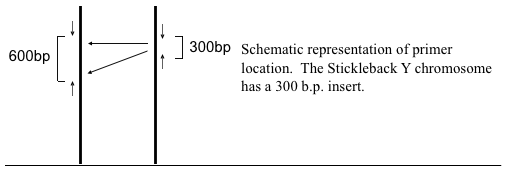
\includegraphics{05_Vertebrate_Experiment/./images/sd_image1.png}

}

\caption{Image \#1 - will be inserted later}

\end{figure}

\begin{itemize}
\tightlist
\item
  Extract DNA into 250µl final volume
\end{itemize}

\hypertarget{pcr-recipe-1x}{%
\subsection{PCR recipe (1X)}\label{pcr-recipe-1x}}

\begin{longtable}[]{@{}llc@{}}
\toprule\noalign{}
Reagent & Concentration & Volume \\
\midrule\noalign{}
\endhead
\bottomrule\noalign{}
\endlastfoot
2X turbo mix & & 10µl \\
GA1 F primer & 10µM & .25µl \\
GA1 R primer & 10µM & .25µl \\
Taq & & .25µl \\
npH\textsubscript{2}O & & 7.25µl \\
DNA & & 2.0µl \\
\textbf{TOTAL} & & \textbf{20µl} \\
\end{longtable}

\begin{itemize}
\tightlist
\item
  After all ingredients are added to a PCR tube put a 10µl drop of
  mineral oil on top.
\end{itemize}

\hypertarget{pcr-reaction-protocol}{%
\subsection{PCR reaction protocol}\label{pcr-reaction-protocol}}

\begin{itemize}
\tightlist
\item
  94˙C -- 5 minutes
\item
  94˙C -- 50 seconds
\item
  44˙C -- 50 seconds (44 cycles)
\item
  72˙C -- 1:20 minutes
\item
  72˙C -- 10 minutes
\end{itemize}

\hypertarget{run-pcr-products-on-a-2-gel}{%
\subsection{Run PCR products on a 2\%
gel}\label{run-pcr-products-on-a-2-gel}}

\begin{figure}

{\centering 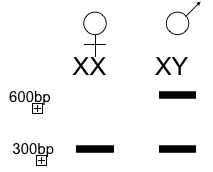
\includegraphics{05_Vertebrate_Experiment/./images/sd_image2.png}

}

\caption{Image \#2 - will be inserted later}

\end{figure}

\hypertarget{sec-vert_exp_steroid_measure}{%
\chapter{Steroid Measurement}\label{sec-vert_exp_steroid_measure}}

\hypertarget{introduction-60}{%
\section{Introduction}\label{introduction-60}}

\begin{itemize}
\tightlist
\item
  \textbf{Purpose}: This procedure describes the technique of how to
  measure steroids in water that has been occupied by fish.
\item
  \textbf{Procedure Type}: Vert Experiment
\item
  \textbf{Species}:

  \begin{itemize}
  \tightlist
  \item
    Threespine stickleback, (\emph{Gasterosteus aculeatus}),
  \item
    Bay pipefish, (\emph{Syngnathus leptorhyncus}),
  \item
    Gulf pipefish (\emph{Syngnathus scovelli})
  \item
    Zebrafish, (\emph{Danio rerio}),
  \end{itemize}
\item
  \textbf{Author}: xxx
\item
  \textbf{Date Created}: xxx
\end{itemize}

\hypertarget{materials}{%
\section{Materials:}\label{materials}}

\begin{itemize}
\tightlist
\item
  150 ml glass beaker
\item
  C18 solid phase extraction (SPE) cartridges containing octadecylsilane
  (Sep-pak Plus, Waters Ltd., Watford, UK)
\end{itemize}

\hypertarget{solutions-52}{%
\section{Solutions}\label{solutions-52}}

\begin{itemize}
\tightlist
\item
  5 ml of distilled water
\item
  5 ml ethyl acetate
\item
  1 ml of RIA buffer (0.5 M phosphate buffer containing 0.2\% bovine
  serum albumen, 0.8\% sodium chloride, 0.03\% EDTA and 0.01\% sodium
  azide)
\item
  \textsuperscript{3}H-labeled steroids for 11-KT are purchased directly
  from Amersham Biosciences, UK (Scott et al., 2005)
\end{itemize}

\hypertarget{procedure-56}{%
\section{Procedure}\label{procedure-56}}

\hypertarget{water-collection}{%
\subsection{Water Collection}\label{water-collection}}

\begin{itemize}
\tightlist
\item
  The fish is placed in a 150-ml glass beaker with 50 ml of fresh water
  (the same source as used for aquaria) for 30 min.
\item
  In the case of male sticklebacks in individual tanks, the beaker is
  placed on a support in the tank to minimise the potential confinement
  stress.
\item
  After the 30-min period the fish is released in its tank.
\item
  If not able to pump the water sample immediately, pour the conditioned
  water into a 50-ml polypropylene centrifuge tube and store at 4°C (up
  to 1hour) or -20°C.
\end{itemize}

\hypertarget{steroid-extraction}{%
\subsection{Steroid Extraction}\label{steroid-extraction}}

\begin{itemize}
\tightlist
\item
  Water samples are pumped through C18 solid phase extraction (SPE)
  cartridges containing octadecylsilane (Sep-pak Plus, Waters Ltd.,
  Watford, UK).
\item
  The cartridges are first washed with 5 ml of 100\% methanol and then 5
  ml of distilled water.
\item
  As the volume of water is small (50ml) no filter is used.
\item
  The water samples are transferred into 60-ml syringes (BD Plastipak),
  drawn by vacuum through the cartridges, and 5 ml of distilled water is
  pushed through the cartridges and blown out.
\item
  The steroids are extracted with 5 ml ethyl acetate, which was then
  dried down to dryness under a stream of nitrogen (45°C).
\item
  Then, 1 ml of RIA buffer (0.5 M phosphate buffer containing 0.2\%
  bovine serum albumen, 0.8\% sodium chloride, 0.03\% EDTA and 0.01\%
  sodium azide) is added and the tubes stored at -20°C until RIAs.
\end{itemize}

\hypertarget{radioimmunoassay}{%
\subsection{Radioimmunoassay}\label{radioimmunoassay}}

\begin{itemize}
\tightlist
\item
  \textsuperscript{3}H-labeled steroids for 11-KT are purchased directly
  from Amersham Biosciences, UK (Scott et al., 2005).
\item
  Antisera came from previously recorded sources (see (Lower et al.,
  2004) where the same sort of study was carried out).
\item
  The RIA procedure has been described previously (Scott et al., 1980;
  Scott et al., 1984; Scott et al., 1982).
\item
  Briefly, 100 μl aliquots from the water sample extract or standards
  are transferred to assay tubes.
\item
  Labelled steroids and antisera are added in a further 100 μl of assay
  buffer, and the tubes left to incubate overnight at 4°C.
\item
  Free and bound labelled steroids are separated with dextran-coated
  charcoal by centrifugation (2,500 rpm for 12 min at 4ºC).
\item
  The supernatant is poured into suitable vials and 7 ml of
  scintillation fluid is added.
\item
  Each tube is then counted for 5 min in the counter (Beckman LS 6500).
\item
  The detection limit of the assays varied between 1 and 10 pg/ assay
  tube (i.e.~10 pg/ 100μl assay buffer).
\end{itemize}

\hypertarget{associated-papers-36}{%
\section{Associated Papers}\label{associated-papers-36}}

\begin{itemize}
\tightlist
\item
  LOWER, N., SCOTT, A. P. \& MOORE, A. (2004). Release of sex steroids
  into the water by roach. --- Journal of Fish Biology 64, 16-33.
\item
  SCOTT, A. P., BYE, V. J., BAYNES, S. M. \& SPRINGATE, J. R. C. (1980).
  Seasonal variations in plasma concentrations of 11-ketotestosterone
  and testosterone in male rainbow trout, Salmo gairdnerii Richardson.
  --- Journal of Fish Biology 17, 495-505.
\item
  SCOTT, A. P., SHELDRICK, E. L. \& FLINT, A.P.F. (1982). Measurement of
  17a,20b-dihydroxy-4-pregnen-3-one in plasma of trout (Salmo gairdneri
  Richardson): seasonal changes and response to salmon pituitary
  extract. --- General and Comparative Endocrinology 46, 444-451
\item
  SCOTT, A. P., MACKENZIE, D. S. \& STACEY, N. E. (1984). Endocrine
  changes during natural spawning in the white sucker, Catostomus
  commersoni. II. Steroid hormones. --- General and Comparative
  Endocrinology 56, 349-359.
\item
  SCOTT, A. P., PINILLOS, M. L. \& HUERTAS, M. (2005). The rate of
  uptake of sex steroids from water by Tinca tinca is influenced by
  their affinity for sex steroid binding protein in plasma. --- Journal
  of Fish Biology 67, 182-200
\end{itemize}

\hypertarget{sec-vert_exp-syngnathid}{%
\chapter{Pipefish backfill labeling if hindbrain
neurons}\label{sec-vert_exp-syngnathid}}

\hypertarget{introduction-61}{%
\section{Introduction}\label{introduction-61}}

\begin{itemize}
\tightlist
\item
  \textbf{Purpose}: This procedure descibes how to backfill nerons of
  pipefish.
\item
  \textbf{Procedure Type}: Experimental
\item
  \textbf{Species}:

  \begin{itemize}
  \tightlist
  \item
    Bay pipefish, (\emph{Syngnathus leptorhyncus})
  \item
    Gulf pipefish (\emph{Syngnathus scovelli})
  \end{itemize}
\item
  \textbf{Author}: Susie Bassham
\item
  \textbf{Date Created}: xxx
\end{itemize}

\hypertarget{materials-56}{%
\section{Materials}\label{materials-56}}

\begin{itemize}
\tightlist
\item
  Antibiotic (Cell Culture anti-biotic/mycotic from Gibco-BRL
  (15240-096) 100x Concentration) Stickleback embryo medium
\item
  Obsidian
\item
  Rhodamine
\item
  DiO lipophilic carbocyanine dye
\end{itemize}

\hypertarget{solutions-53}{%
\section{Solutions}\label{solutions-53}}

\begin{itemize}
\tightlist
\item
  MS-222 Anesthesia solution \{\#sec-husbandry\_anesth\_pipefish\}
\item
  MS-222 Euthanasia solution \{\#sec-vert\_husb-euthanasia\_syngnathid\}
\end{itemize}

\hypertarget{procedure-57}{%
\section{Procedure}\label{procedure-57}}

\begin{enumerate}
\def\labelenumi{\arabic{enumi}.}
\tightlist
\item
  Sedate Larval fish in MS222 in sterile filtered seawater + antibiotic
  (Cell Culture anti-biotic/mycotic from Gibco-BRL (15240-096) 100x
  Concentration).
\item
  Use a obsidian glass flake, an extremely sharp scalpel, an incision
  will be made from the dorsal side, extending ventrally just through
  the spinal cord.
\item
  Use a fine insect pin to apply dried crystals of rhodamine dextran,
  DiO, or similar reagent to the cut spinal cord.
\item
  Continuously sedate larvae. Euthanized with MS222 and fixed 5 to 16
  hours after surgery prior to imaging.
\end{enumerate}

\hypertarget{associated-papers-37}{%
\section{Associated Papers}\label{associated-papers-37}}

\begin{itemize}
\tightlist
\item
  xxx
\item
  xxx
\item
  xxx
\item
  xxx
\end{itemize}

\hypertarget{sec-vert_exp_live_alizarin_syngnathid}{%
\chapter{Live syngnathid alizarin
staining}\label{sec-vert_exp_live_alizarin_syngnathid}}

\hypertarget{introduction-62}{%
\section{Introduction}\label{introduction-62}}

\begin{itemize}
\tightlist
\item
  \textbf{Purpose}: This procedure describes how to live stain
  syngnathid with alizarin.
\item
  \textbf{Procedure Type}: Vert Experimental
\item
  \textbf{Species}:

  \begin{itemize}
  \tightlist
  \item
    Bay pipefish, (\emph{Syngnathus leptorhyncus})
  \item
    Gulf pipefish (\emph{Syngnathus scovelli})
  \end{itemize}
\item
  \textbf{Author}: Mark Currey
\item
  \textbf{Date Created}: January 01, 2024
\end{itemize}

\hypertarget{materials-57}{%
\section{Materials}\label{materials-57}}

\begin{itemize}
\tightlist
\item
  Large Petri Dish
\item
  xxx
\item
  xxx
\item
  xxx
\end{itemize}

\hypertarget{solutions-54}{%
\section{Solutions}\label{solutions-54}}

\begin{itemize}
\tightlist
\item
  Alizarin stock solutions: 0.5g Alizarin red in 100ml or in 50ml in
  sterile water (SIGMA cat\# A5533 Alizarin Red S, certified).
\item
  Staining Solution:

  \begin{itemize}
  \tightlist
  \item
    25 ppt Instant Ocean
  \item
    Add 10 ml 0.5\% or 1\% Alizarin Stock in sterile water for final
    concentrations of 0.005\% or 0.01\%.
  \item
    Adjust to pH 7.5 with NaOH
  \end{itemize}
\item
  For 50 ml (enough for 100mm diameter petri dish):

  \begin{itemize}
  \tightlist
  \item
    49.5 ml Embryo medium
  \item
    Add 500 µl 0.5\% or 1\% Alizarin Stock in sterile water
  \item
    Adjust to pH 7.5 with NaOH
  \end{itemize}
\item
  MESAB anesthesia strength \{\#sec-husbandry\_anesth\_pipefish\}
\item
  MESAB euthanisia strength \{\#sec-husbandry\_adult\_syng\_euth\}
\end{itemize}

\hypertarget{procedure-58}{%
\section{Procedure}\label{procedure-58}}

\begin{enumerate}
\def\labelenumi{\arabic{enumi}.}
\tightlist
\item
  Place fish into a container containing stain for 1-2 hours for larvae
  to overnight for juveniles or adult fish in the dark. We have found
  that fish do not experience adverse effects from being exposed to
  stain. Monitor fish every 30-60 minutes if possible. To de-stain,
  rinse thoroughly with embryo medium by placing fish into container of
  embryo medium without stain for 30 minutes; background continues to go
  down with time. Move on to DASPEI live staining if desired (see DASPEI
  live staining SOP) or anesthetize until the fish reaches a light plane
  of anesthesia (i.e.~movement has slowed down enough that the fish can
  be safely handled) and observe/image.
\item
  Bone fluorescence will decrease over time, so plan on imaging the same
  day if possible.
\item
  Keep fish in the dark as much as is reasonably convenient.
\item
  After fish has been observed/imaged place in a container of fish
  water. Monitor fish every 5-10 minutes until the fish is revived. Once
  fish is revived place back on the fish system and monitor during daily
  health checks. If the fish is to be fixed for post mortem experiments
  place fish directly into euthanasia MS222 solution and follow
  \{\#sec-husbandry\_adult\_syng\_euth\}.
\end{enumerate}

\hypertarget{associated-papers-38}{%
\section{Associated Papers}\label{associated-papers-38}}

\begin{itemize}
\tightlist
\item
  xxx
\item
  xxx
\item
  xxx
\item
  xxx
\end{itemize}

\hypertarget{sec-vert_exp_live_calcein_syngnathid}{%
\chapter{Live syngnathid calcein
staining}\label{sec-vert_exp_live_calcein_syngnathid}}

\hypertarget{introduction-63}{%
\section{Introduction}\label{introduction-63}}

\begin{itemize}
\tightlist
\item
  \textbf{Purpose}: This procedure describes how to live stain
  syngnathid with calcein.
\item
  \textbf{Procedure Type}: Vert Experimental
\item
  \textbf{Species}:

  \begin{itemize}
  \tightlist
  \item
    Bay pipefish, (\emph{Syngnathus leptorhyncus})
  \item
    Gulf pipefish (\emph{Syngnathus scovelli})
  \end{itemize}
\item
  \textbf{Author}: Mark Currey
\item
  \textbf{Date Created}: January 01, 2024
\end{itemize}

\hypertarget{materials-58}{%
\section{Materials}\label{materials-58}}

\begin{itemize}
\tightlist
\item
  Petri dishes and/or 1 L tanks
\item
  Calcein (Molecular Probes; cat. C481)
\end{itemize}

\hypertarget{solutions-55}{%
\section{Solutions}\label{solutions-55}}

\begin{itemize}
\tightlist
\item
  MESAB anesthesia strength \{\#sec-husbandry\_anesth\_pipefish\}
\item
  MESAB euthanisia strength \{\#sec-husbandry\_adult\_syng\_euth\}
\item
  25 ppt Instant Ocean
\item
  10\% NaOH
\item
  Stain Solution:

  \begin{itemize}
  \tightlist
  \item
    0.005 to 0.05\% calcein in sea water.
  \item
    Adjust pH to 8.2 with NaOH
  \item
    Make fresh, keep in dark.
  \end{itemize}
\end{itemize}

\hypertarget{procedure-59}{%
\section{Procedure}\label{procedure-59}}

\begin{enumerate}
\def\labelenumi{\arabic{enumi}.}
\tightlist
\item
  Place fish into a container containing stain for 1-2 hours for larvae
  to overnight for juveniles or adult fish in the dark. We have found
  that fish do not experience adverse effects from being exposed to
  stain. Monitor fish every 30-60 minutes if possible. To de-stain,
  rinse thoroughly with embryo medium by placing fish into container of
  embryo medium without stain for 30 minutes; background continues to go
  down with time. Move on to DASPEI live staining if desired (see DASPEI
  live staining SOP) or anesthetize until the fish reaches a light plane
  of anesthesia (i.e.~movement has slowed down enough that the fish can
  be safely handled) and observe/image.
\item
  Bone fluorescence will decrease over time, so plan on imaging the same
  day if possible.
\item
  Keep fish in the dark as much as is reasonably convenient.
\item
  After fish has been observed/imaged place in a container of fish
  water. Monitor fish every 5-10 minutes until the fish is revived. Once
  fish is revived place back on the fish system and monitor during daily
  health checks. If the fish is to be fixed for post mortem experiments
  place fish directly into euthanasia MS222 solution and follow the
  euthanasia SOP.
\end{enumerate}

\hypertarget{associated-papers-39}{%
\section{Associated Papers}\label{associated-papers-39}}

\begin{itemize}
\tightlist
\item
  xxx
\item
  xxx
\item
  xxx
\item
  xxx
\end{itemize}

\hypertarget{sec-vert_exp_live_daspei_syngnathid}{%
\chapter{Live syngnathid DASPEI
staining}\label{sec-vert_exp_live_daspei_syngnathid}}

\hypertarget{introduction-64}{%
\section{Introduction}\label{introduction-64}}

\begin{itemize}
\tightlist
\item
  \textbf{Purpose}: This procedure describes how to live stain
  syngnathid with DASPEI.
\item
  \textbf{Procedure Type}: Vert Experimental
\item
  \textbf{Species}:

  \begin{itemize}
  \tightlist
  \item
    Bay pipefish, (\emph{Syngnathus leptorhyncus})
  \item
    Gulf pipefish (\emph{Syngnathus scovelli})
  \end{itemize}
\item
  \textbf{Author}: Susie Bassham
\item
  \textbf{Date Created}: October 25, 2021; adapted from DOI:
  10.1007/s10162-002-3022-x
\end{itemize}

\hypertarget{materials-59}{%
\section{Materials}\label{materials-59}}

\begin{itemize}
\tightlist
\item
  Petri dishes and/or 1 L tanks
\item
  DASPEI (Sigma Aldrich; cat. D3418)
\end{itemize}

\hypertarget{solutions-56}{%
\section{Solutions}\label{solutions-56}}

\begin{itemize}
\tightlist
\item
  MESAB anesthesia strength \{\#sec-husbandry\_anesth\_pipefish\}
\item
  MESAB euthanisia strength \{\#sec-husbandry\_adult\_syng\_euth\}
\item
  25 ppt Instant Ocean
\item
  Staining Solution:

  \begin{itemize}
  \tightlist
  \item
    0.005\% DASPEI in sea water
  \end{itemize}
\end{itemize}

\hypertarget{procedure-60}{%
\section{Procedure}\label{procedure-60}}

\begin{enumerate}
\def\labelenumi{\arabic{enumi}.}
\tightlist
\item
  Stain larvae in Petri dishes and juveniles/adults in 1 L tanks
  containing stain solution for 5 to 75 min in the dark; stagger so that
  no fish stain longer than this before imaging. Rinse for 20 to 60 min
  in container of sea water without DASPEI to reduce background.
\item
  Keep fish in the dark as much as is reasonably convenient through
  procedures. Monitor fish every 15-30 minutes.
\item
  Anesthetize until the fish reaches a light plane of anesthesia
  (i.e.~movement has slowed down enough that the fish can be safely
  handled) and observe/image fluorescence immediately.
\item
  After fish has been observed/imaged place in a container of fish
  water. Monitor fish every 5-10 minutes until the fish is revived. Once
  fish is revived place back on the fish system and monitor during daily
  health checks. If the fish is to be fixed for post mortem experiments
  place fish directly into euthanasia MS222 solution and follow the
  euthanasia SOP.
\item
  Staining solution can be stored at 4C and reused.
\end{enumerate}

\hypertarget{associated-papers-40}{%
\section{Associated Papers}\label{associated-papers-40}}

\begin{itemize}
\tightlist
\item
  xxx
\item
  xxx
\item
  xxx
\item
  xxx
\end{itemize}

\part{Daphnia Husbandry}

This section of the manual contains protocols for the safe and ethical
husbandry and use of invertebrate animals, particular the nematode worm
\emph{C. remanei} and water fleas of the genus \emph{Daphnia}

\hypertarget{sec-Daphnia}{%
\chapter{Placeholder\_Daphnia}\label{sec-Daphnia}}

\hypertarget{xxx-2}{%
\section{xxx}\label{xxx-2}}

xxxx

\hypertarget{xxx-3}{%
\subsection{xxx}\label{xxx-3}}

xxxxx

\part{Common Recipes}

This section of the book contains common recipes used for solutions and
reagents across other protocols

\hypertarget{sec-recipe_dietrichs_fix}{%
\chapter{Dietrich's Fixative (EM)}\label{sec-recipe_dietrichs_fix}}

\hypertarget{introduction-65}{%
\section{Introduction}\label{introduction-65}}

\begin{itemize}
\tightlist
\item
  \textbf{Purpose}: Recipe for Dietrich's fixative
\item
  \textbf{Procedure Type}: recipe
\item
  \textbf{Species}:

  \begin{itemize}
  \tightlist
  \item
    Threespine stickleback, (\emph{Gasterosteus aculeatus})
  \item
    Bay pipefish, (\emph{Syngnathus leptorhyncus})
  \item
    Gulf pipefish (\emph{Syngnathus scovelli})
  \end{itemize}
\item
  \textbf{Author}: Mark Currey
\item
  \textbf{Date Created}: February 29, 2024
\end{itemize}

When fixing sentinel fish use Dieterich's fixative.

\hypertarget{materials-60}{%
\section{Materials}\label{materials-60}}

\begin{itemize}
\tightlist
\item
  Ethanol (95\%)
\item
  Formalin (Formaldehyde 37\% solution, histological grade, contains
  10-15\% methanol, Sigma \# F1635)
\item
  Glacial Acetic Acid
\item
  Distilled WaterSolutions
\end{itemize}

\hypertarget{procedure-61}{%
\section{Procedure}\label{procedure-61}}

\begin{enumerate}
\def\labelenumi{\arabic{enumi}.}
\tightlist
\item
  Prepare Dietrich's Fixative (100 ml), mix: - 30 ml Ethanol (95\%) - 10
  ml Formalin (Formaldehyde 37\% solution, histological grade, contains
  10-15\% methanol, Sigma \# F1635) - 2 ml Glacial Acetic Acid - 58 ml
  Distilled Water
\item
  Store fixative at room temperature.
\end{enumerate}

\hypertarget{associated-papers-41}{%
\section{Associated Papers}\label{associated-papers-41}}

\begin{itemize}
\tightlist
\item
  xxx
\item
  xxx
\item
  xxx
\item
  xxx
\end{itemize}

\hypertarget{sec-general_recipe_embryo_medium}{%
\chapter{Stickleback Embryo Medium
(EM)}\label{sec-general_recipe_embryo_medium}}

\hypertarget{introduction-66}{%
\section{Introduction}\label{introduction-66}}

\begin{itemize}
\tightlist
\item
  \textbf{Purpose}: Recipe for embryo medium\\
\item
  \textbf{Procedure Type}: recipe
\item
  \textbf{Species}:

  \begin{itemize}
  \tightlist
  \item
    Threespine stickleback, (\emph{Gasterosteus aculeatus})
  \end{itemize}
\item
  \textbf{Author}: Mark Currey
\item
  \textbf{Date Created}: January 1, 2004
\end{itemize}

\hypertarget{materials-61}{%
\section{Materials}\label{materials-61}}

\begin{itemize}
\tightlist
\item
  Instant Ocean Salt
\item
  Baking Soda
\item
  nano pure water (npH2O)
\end{itemize}

\hypertarget{solutions-57}{%
\section{Solutions}\label{solutions-57}}

\begin{itemize}
\tightlist
\item
  none
\end{itemize}

\hypertarget{procedure-62}{%
\section{Procedure}\label{procedure-62}}

For 2 liters: 1. Add 8g Instant Ocean to 2 liters of npH2O 2. Add
\textasciitilde0.5g baking soda 3. Check pH and adjust to 7.0 -- 8.0

Salt and baking soda are located in containers near the weigh station.
Rinse 2 liter flasks with DI water between uses.

\hypertarget{associated-papers-42}{%
\section{Associated Papers}\label{associated-papers-42}}

\begin{itemize}
\tightlist
\item
  xxx
\item
  xxx
\item
  xxx
\item
  xxx
\end{itemize}

\hypertarget{sec-general_recipe_ginzbergs_ringers}{%
\chapter{Ginzberg's Ringer
Solution}\label{sec-general_recipe_ginzbergs_ringers}}

\hypertarget{introduction-67}{%
\section{Introduction}\label{introduction-67}}

\begin{itemize}
\tightlist
\item
  \textbf{Purpose}: Recipe for making ginzberg's ringers solution\\
\item
  \textbf{Procedure Type}: recipe
\item
  \textbf{Species}:

  \begin{itemize}
  \tightlist
  \item
    Threespine stickleback, (\emph{Gasterosteus aculeatus})
  \end{itemize}
\item
  \textbf{Author}: Mark Currey
\item
  \textbf{Date Created}: January 1, 2004
\end{itemize}

\hypertarget{materials-62}{%
\section{Materials}\label{materials-62}}

\begin{itemize}
\tightlist
\item
  NaCl
\item
  KCl
\item
  CaCl2
\item
  NaHCO3
\item
  npH2O
\end{itemize}

All of these reagents should be located in the chemical cabinet.

\hypertarget{solutions-58}{%
\section{Solutions}\label{solutions-58}}

\begin{itemize}
\tightlist
\item
  none
\end{itemize}

\hypertarget{procedure-63}{%
\section{Procedure}\label{procedure-63}}

For 1000 mls, mix: 1. Mix solids into 750 ml of npH2O - 6.6g NaCl -
0.25g KCl - 0.3g CaCl2 - 0.2g NaHCO3 2. Bring to 1 liter total volume
with npH2O. 3. Store at 4° C.

\hypertarget{associated-papers-43}{%
\section{Associated Papers}\label{associated-papers-43}}

\begin{itemize}
\tightlist
\item
  xxx
\item
  xxx
\item
  xxx
\item
  xxx
\end{itemize}

\hypertarget{sec-general_recipe_mesab}{%
\chapter{Mesab Stock (EM)}\label{sec-general_recipe_mesab}}

\hypertarget{introduction-68}{%
\section{Introduction}\label{introduction-68}}

\begin{itemize}
\tightlist
\item
  \textbf{Purpose}: Recipe for making a mesab stock solution\\
\item
  \textbf{Procedure Type}: recipe
\item
  \textbf{Species}:

  \begin{itemize}
  \tightlist
  \item
    Threespine stickleback, (\emph{Gasterosteus aculeatus})
  \item
    Bay pipefish, (\emph{Syngnathus leptorhyncus})
  \item
    Gulf pipefish (\emph{Syngnathus scovelli})
  \end{itemize}
\item
  \textbf{Author}: Mark Currey
\item
  \textbf{Date Created}: January 1, 2004
\end{itemize}

Mesab also known as Tricaine must be pharmaceutical-grade. We use
tricaine purchased from Pentair, manufactured by Western Chemical and
FDA approved. Tricaine (3-amino benzoic acid ethyl lester also called
ethyl m-aminoboenzoate) comes in a powdered form. Purchase the smallest
amount possible because tricaine expires quickly.

\hypertarget{materials-63}{%
\section{Materials}\label{materials-63}}

\begin{itemize}
\tightlist
\item
  Mesab, a.k.a. MS222, tricaine, or 3-aminobenzoic acid ethyl ester
\item
  1 M Tris (pH 9)
\item
  DD water
\end{itemize}

\hypertarget{solutions-59}{%
\section{Solutions}\label{solutions-59}}

\begin{itemize}
\tightlist
\item
  none
\end{itemize}

\hypertarget{procedure-64}{%
\section{Procedure}\label{procedure-64}}

For 1 liter, mix: 1. 4 g tricaine powder 2. 979 ml DD water 3.
\textasciitilde21 ml 1 M Tris (pH 9). 4. Adjust pH to \textasciitilde7.
5. Aliquot in 50 ml tubes, label with MESAB Stock Solution 4g/L, and
store in a -20 freezer.

\hypertarget{associated-papers-44}{%
\section{Associated Papers}\label{associated-papers-44}}

\begin{itemize}
\tightlist
\item
  xxx
\item
  xxx
\item
  xxx
\item
  xxx
\end{itemize}

\hypertarget{sec-general_recipe_testes_solution}{%
\chapter{Testes Storage
Solution}\label{sec-general_recipe_testes_solution}}

\hypertarget{introduction-69}{%
\section{Introduction}\label{introduction-69}}

\begin{itemize}
\tightlist
\item
  \textbf{Purpose}: Recipe for making testes storage solution\\
\item
  \textbf{Procedure Type}: recipe
\item
  \textbf{Species}:

  \begin{itemize}
  \tightlist
  \item
    Threespine stickleback, (\emph{Gasterosteus aculeatus})
  \end{itemize}
\item
  \textbf{Author}: Mark Currey
\item
  \textbf{Date Created}: January 1, 2004
\end{itemize}

\hypertarget{materials-64}{%
\section{Materials}\label{materials-64}}

\begin{itemize}
\tightlist
\item
  Gentamycin (antimycotic) (Stock -- 10 mg/ml)*
\item
  Cell Culture anti-biotic/mycotic from Gibco-BRL (15240-096) 100x
  Concentration
\end{itemize}

Both of these reagents are located in separate boxes in the scientific
-20° C freezer. They are partitioned into 100μl aliquots.

\hypertarget{solutions-60}{%
\section{Solutions}\label{solutions-60}}

\begin{itemize}
\tightlist
\item
  Ginzberg's Ringers \{\#sec-general\_recipe\_ginzbergs\_ringers\}
\end{itemize}

\hypertarget{procedure-65}{%
\section{Procedure}\label{procedure-65}}

For 100 mls, mix: 1. Add 100μl of Gentamycin and 100μl of
Anti-biotic/mycotic to 100ml of Ginzburg's Ringers solution. 2. Store at
4° C.

\hypertarget{associated-papers-45}{%
\section{Associated Papers}\label{associated-papers-45}}

\begin{itemize}
\tightlist
\item
  xxx
\item
  xxx
\item
  xxx
\item
  xxx
\end{itemize}

\hypertarget{recipe---8-paraformaldehyde-stock-solution-sec-general_recipe_8pfa}{%
\chapter{Recipe - 8\% Paraformaldehyde Stock Solution
\{\#sec-general\_recipe\_8\%PFA\}}\label{recipe---8-paraformaldehyde-stock-solution-sec-general_recipe_8pfa}}

\hypertarget{introduction-70}{%
\section{Introduction}\label{introduction-70}}

\begin{itemize}
\tightlist
\item
  \textbf{Purpose}: Recipe for 8\% Paraformaldehyde (PFA) Stock
  Solution\\
\item
  \textbf{Procedure Type}: recipe
\item
  \textbf{Species}:

  \begin{itemize}
  \tightlist
  \item
    Threespine stickleback, (\emph{Gasterosteus aculeatus})
  \item
    Bay pipefish, (\emph{Syngnathus leptorhyncus})
  \item
    Gulf pipefish (\emph{Syngnathus scovelli})
  \end{itemize}
\item
  \textbf{Author}: Mark Currey
\item
  \textbf{Date Created}: February 29, 2024
\end{itemize}

Use gloves and PPE when handling paraformaldehyde

\hypertarget{materials-65}{%
\section{Materials}\label{materials-65}}

\begin{verbatim}
-   paraformaldehyde
\end{verbatim}

\begin{tcolorbox}[enhanced jigsaw, bottomtitle=1mm, rightrule=.15mm, toptitle=1mm, opacitybacktitle=0.6, bottomrule=.15mm, titlerule=0mm, coltitle=black, leftrule=.75mm, arc=.35mm, colback=white, colframe=quarto-callout-note-color-frame, left=2mm, colbacktitle=quarto-callout-note-color!10!white, title=\textcolor{quarto-callout-note-color}{\faInfo}\hspace{0.5em}{Note}, toprule=.15mm, opacityback=0, breakable]

Paraformaldehyde can be found in the chemical cabinet.

\end{tcolorbox}

\begin{verbatim}
-   Distilled Water
\end{verbatim}

\hypertarget{solutions-61}{%
\section{Solutions}\label{solutions-61}}

\begin{verbatim}
-  10N NaOH
-  20% HCl
\end{verbatim}

\hypertarget{procedure-66}{%
\section{Procedure}\label{procedure-66}}

USE A FUME HOOD!

\begin{enumerate}
\def\labelenumi{\arabic{enumi}.}
\tightlist
\item
  Add 40 g Paraformaldehyde to 450 ml distilled water (or scale for
  desired final volume).
\item
  Add 1 ul of 10 N NaOH per ml of water (i.e.~500 ul for 500 ml).
\item
  Apply medium heat while stirring at medium speed to dissolve - approx
  15-20 min. Solution should not go above 60º C. Eventually, granules
  will fully dissolve and the solution will become translucent.
\end{enumerate}

DO NOT LET THE SOLUTION STIR BEYOND THIS POINT - it will form a fuzzy
precipitate that reduces the solution strength after filtering.

\begin{enumerate}
\def\labelenumi{\arabic{enumi}.}
\setcounter{enumi}{3}
\tightlist
\item
  Once the granules have dissolved and the solution clears, turn off the
  heat.
\item
  Equilibrate to pH 7.4 with approx 1.5 ml of 20\% HCl (or scale,
  depending on target volume). Bring volume to 500 ml (or scaled volume)
  with distilled water.\\
\item
  Filter while still warm to 0.45 um (or 0.2 um).\\
\item
  Aliquot and store at -20º C.
\end{enumerate}

\hypertarget{associated-papers-46}{%
\section{Associated Papers}\label{associated-papers-46}}

\begin{itemize}
\tightlist
\item
  xxx
\item
  xxx
\item
  xxx
\item
  xxx
\end{itemize}

\part{Bioinformatic}

This ection of the book contains protocols for basic bioinformatic
skills such as using our laboratory cluster `Genome', as well as our
account Nereus on the UO supercomputer Talapas.

Note that there are several appendices that contain greater details and
training on things such as the use of command line, R and Python,
markdown and literature programming, and documentation using Quarto and
Jupyter notebooks.

See Knuth (1984) for additional discussion of literate programming.

\hypertarget{sec-base-r}{%
\chapter{A field guide to base R}\label{sec-base-r}}

\hypertarget{introduction-71}{%
\section{Introduction}\label{introduction-71}}

To finish off the programming section, we're going to give you a quick
tour of the most important base R functions that we don't otherwise
discuss in the book. These tools are particularly useful as you do more
programming and will help you read code you'll encounter in the wild.

This is a good place to remind you that the tidyverse is not the only
way to solve data science problems. We teach the tidyverse in this book
because tidyverse packages share a common design philosophy, increasing
the consistency across functions, and making each new function or
package a little easier to learn and use. It's not possible to use the
tidyverse without using base R, so we've actually already taught you a
\textbf{lot} of base R functions: from \texttt{library()} to load
packages, to \texttt{sum()} and \texttt{mean()} for numeric summaries,
to the factor, date, and POSIXct data types, and of course all the basic
operators like \texttt{+}, \texttt{-}, \texttt{/}, \texttt{*},
\texttt{\textbar{}}, \texttt{\&}, and \texttt{!}. What we haven't
focused on so far is base R workflows, so we will highlight a few of
those in this chapter.

After you read this book, you'll learn other approaches to the same
problems using base R, data.table, and other packages. You'll
undoubtedly encounter these other approaches when you start reading R
code written by others, particularly if you're using StackOverflow. It's
100\% okay to write code that uses a mix of approaches, and don't let
anyone tell you otherwise!

In this chapter, we'll focus on four big topics: subsetting with
\texttt{{[}}, subsetting with \texttt{{[}{[}} and \texttt{\$}, the apply
family of functions, and \texttt{for} loops. To finish off, we'll
briefly discuss two essential plotting functions.

\hypertarget{prerequisites}{%
\subsection{Prerequisites}\label{prerequisites}}

This package focuses on base R so doesn't have any real prerequisites,
but we'll load the tidyverse in order to explain some of the
differences.

\begin{Shaded}
\begin{Highlighting}[]
\FunctionTok{library}\NormalTok{(tidyverse)}
\end{Highlighting}
\end{Shaded}

\hypertarget{sec-subset-many}{%
\section{\texorpdfstring{Selecting multiple elements with
\texttt{{[}}}{Selecting multiple elements with {[}}}\label{sec-subset-many}}

\texttt{{[}} is used to extract sub-components from vectors and data
frames, and is called like \texttt{x{[}i{]}} or \texttt{x{[}i,\ j{]}}.
In this section, we'll introduce you to the power of \texttt{{[}}, first
showing you how you can use it with vectors, then how the same
principles extend in a straightforward way to two-dimensional (2d)
structures like data frames. We'll then help you cement that knowledge
by showing how various dplyr verbs are special cases of \texttt{{[}}.

\hypertarget{subsetting-vectors}{%
\subsection{Subsetting vectors}\label{subsetting-vectors}}

There are five main types of things that you can subset a vector with,
i.e., that can be the \texttt{i} in \texttt{x{[}i{]}}:

\begin{enumerate}
\def\labelenumi{\arabic{enumi}.}
\item
  \textbf{A vector of positive integers}. Subsetting with positive
  integers keeps the elements at those positions:

\begin{Shaded}
\begin{Highlighting}[]
\NormalTok{x }\OtherTok{\textless{}{-}} \FunctionTok{c}\NormalTok{(}\StringTok{"one"}\NormalTok{, }\StringTok{"two"}\NormalTok{, }\StringTok{"three"}\NormalTok{, }\StringTok{"four"}\NormalTok{, }\StringTok{"five"}\NormalTok{)}
\NormalTok{x[}\FunctionTok{c}\NormalTok{(}\DecValTok{3}\NormalTok{, }\DecValTok{2}\NormalTok{, }\DecValTok{5}\NormalTok{)]}
\end{Highlighting}
\end{Shaded}

\begin{verbatim}
[1] "three" "two"   "five" 
\end{verbatim}

  By repeating a position, you can actually make a longer output than
  input, making the term ``subsetting'' a bit of a misnomer.

\begin{Shaded}
\begin{Highlighting}[]
\NormalTok{x[}\FunctionTok{c}\NormalTok{(}\DecValTok{1}\NormalTok{, }\DecValTok{1}\NormalTok{, }\DecValTok{5}\NormalTok{, }\DecValTok{5}\NormalTok{, }\DecValTok{5}\NormalTok{, }\DecValTok{2}\NormalTok{)]}
\end{Highlighting}
\end{Shaded}

\begin{verbatim}
[1] "one"  "one"  "five" "five" "five" "two" 
\end{verbatim}
\item
  \textbf{A vector of negative integers}. Negative values drop the
  elements at the specified positions:

\begin{Shaded}
\begin{Highlighting}[]
\NormalTok{x[}\FunctionTok{c}\NormalTok{(}\SpecialCharTok{{-}}\DecValTok{1}\NormalTok{, }\SpecialCharTok{{-}}\DecValTok{3}\NormalTok{, }\SpecialCharTok{{-}}\DecValTok{5}\NormalTok{)]}
\end{Highlighting}
\end{Shaded}

\begin{verbatim}
[1] "two"  "four"
\end{verbatim}
\item
  \textbf{A logical vector}. Subsetting with a logical vector keeps all
  values corresponding to a \texttt{TRUE} value. This is most often
  useful in conjunction with the comparison functions.

\begin{Shaded}
\begin{Highlighting}[]
\NormalTok{x }\OtherTok{\textless{}{-}} \FunctionTok{c}\NormalTok{(}\DecValTok{10}\NormalTok{, }\DecValTok{3}\NormalTok{, }\ConstantTok{NA}\NormalTok{, }\DecValTok{5}\NormalTok{, }\DecValTok{8}\NormalTok{, }\DecValTok{1}\NormalTok{, }\ConstantTok{NA}\NormalTok{)}

\CommentTok{\# All non{-}missing values of x}
\NormalTok{x[}\SpecialCharTok{!}\FunctionTok{is.na}\NormalTok{(x)]}
\end{Highlighting}
\end{Shaded}

\begin{verbatim}
[1] 10  3  5  8  1
\end{verbatim}

\begin{Shaded}
\begin{Highlighting}[]
\CommentTok{\# All even (or missing!) values of x}
\NormalTok{x[x }\SpecialCharTok{\%\%} \DecValTok{2} \SpecialCharTok{==} \DecValTok{0}\NormalTok{]}
\end{Highlighting}
\end{Shaded}

\begin{verbatim}
[1] 10 NA  8 NA
\end{verbatim}

  Unlike \texttt{filter()}, \texttt{NA} indices will be included in the
  output as \texttt{NA}s.
\item
  \textbf{A character vector}. If you have a named vector, you can
  subset it with a character vector:

\begin{Shaded}
\begin{Highlighting}[]
\NormalTok{x }\OtherTok{\textless{}{-}} \FunctionTok{c}\NormalTok{(}\AttributeTok{abc =} \DecValTok{1}\NormalTok{, }\AttributeTok{def =} \DecValTok{2}\NormalTok{, }\AttributeTok{xyz =} \DecValTok{5}\NormalTok{)}
\NormalTok{x[}\FunctionTok{c}\NormalTok{(}\StringTok{"xyz"}\NormalTok{, }\StringTok{"def"}\NormalTok{)]}
\end{Highlighting}
\end{Shaded}

\begin{verbatim}
xyz def 
  5   2 
\end{verbatim}

  As with subsetting with positive integers, you can use a character
  vector to duplicate individual entries.
\item
  \textbf{Nothing}. The final type of subsetting is nothing,
  \texttt{x{[}{]}}, which returns the complete \texttt{x}. This is not
  useful for subsetting vectors, but as we'll see shortly, it is useful
  when subsetting 2d structures like tibbles.
\end{enumerate}

\hypertarget{summary}{%
\section{Summary}\label{summary}}

In this chapter, we've shown you a selection of base R functions useful
for subsetting and iteration. Compared to approaches discussed elsewhere
in the book, these functions tend to have more of a ``vector'' flavor
than a ``data frame'' flavor because base R functions tend to take
individual vectors, rather than a data frame and some column
specification. This often makes life easier for programming and so
becomes more important as you write more functions and begin to write
your own packages.

This chapter concludes the programming section of the book. You've made
a solid start on your journey to becoming not just a data scientist who
uses R, but a data scientist who can \emph{program} in R. We hope these
chapters have sparked your interest in programming and that you're
looking forward to learning more outside of this book.

\part{References\&Notes}

This section of the book contains references and notes for all protocols

\hypertarget{references}{%
\chapter*{References}\label{references}}
\addcontentsline{toc}{chapter}{References}

\markboth{References}{References}

\hypertarget{refs}{}
\begin{CSLReferences}{1}{0}
\leavevmode\vadjust pre{\hypertarget{ref-knuth84}{}}%
Knuth, Donald E. 1984. {``Literate Programming.''} \emph{Comput. J.} 27
(2): 97--111. \url{https://doi.org/10.1093/comjnl/27.2.97}.

\end{CSLReferences}

\hypertarget{notes}{%
\chapter*{Notes}\label{notes}}
\addcontentsline{toc}{chapter}{Notes}

\markboth{Notes}{Notes}

\hypertarget{refs}{}
\begin{CSLReferences}{1}{0}
\leavevmode\vadjust pre{\hypertarget{ref-knuth84}{}}%
Knuth, Donald E. 1984. {``Literate Programming.''} \emph{Comput. J.} 27
(2): 97--111. \url{https://doi.org/10.1093/comjnl/27.2.97}.

\end{CSLReferences}

\cleardoublepage
\phantomsection
\addcontentsline{toc}{part}{Appendices}
\appendix

\hypertarget{sbf1-barcodes-in-96-well-plate}{%
\chapter{Sbf1 Barcodes in 96 Well
Plate}\label{sbf1-barcodes-in-96-well-plate}}

\begin{longtable}[]{@{}
  >{\raggedright\arraybackslash}p{(\columnwidth - 12\tabcolsep) * \real{0.0400}}
  >{\raggedright\arraybackslash}p{(\columnwidth - 12\tabcolsep) * \real{0.0600}}
  >{\raggedright\arraybackslash}p{(\columnwidth - 12\tabcolsep) * \real{0.1133}}
  >{\raggedright\arraybackslash}p{(\columnwidth - 12\tabcolsep) * \real{0.3133}}
  >{\raggedright\arraybackslash}p{(\columnwidth - 12\tabcolsep) * \real{0.0400}}
  >{\raggedright\arraybackslash}p{(\columnwidth - 12\tabcolsep) * \real{0.1133}}
  >{\raggedright\arraybackslash}p{(\columnwidth - 12\tabcolsep) * \real{0.3200}}@{}}
\toprule\noalign{}
\begin{minipage}[b]{\linewidth}\raggedright
well
\end{minipage} & \begin{minipage}[b]{\linewidth}\raggedright
Barcode
\end{minipage} & \begin{minipage}[b]{\linewidth}\raggedright
Name (top)
\end{minipage} & \begin{minipage}[b]{\linewidth}\raggedright
Final top sequence
\end{minipage} & \begin{minipage}[b]{\linewidth}\raggedright
well
\end{minipage} & \begin{minipage}[b]{\linewidth}\raggedright
Name (bottom)
\end{minipage} & \begin{minipage}[b]{\linewidth}\raggedright
Final bottom sequence
\end{minipage} \\
\midrule\noalign{}
\endhead
\bottomrule\noalign{}
\endlastfoot
A1 & AAACGG & SbfI-AAACGG-top &
ACACTCTTTCCCTACACGACGCTCTTCCGATCTAAACGGTGC*A & A1 & SbfI-AAACGG-bot &
/5Phos/CCGTTTAGATCGGAAGAGCGTCGTGTAGGGAAAGAGTGT \\
A2 & AACGTT & SbfI-AACGTT-top &
ACACTCTTTCCCTACACGACGCTCTTCCGATCTAACGTTTGC*A & A2 & SbfI-AACGTT-bot &
/5Phos/AACGTTAGATCGGAAGAGCGTCGTGTAGGGAAAGAGTGT \\
A3 & AACTGA & SbfI-AACTGA-top &
ACACTCTTTCCCTACACGACGCTCTTCCGATCTAACTGATGC*A & A3 & SbfI-AACTGA-bot &
/5Phos/TCAGTTAGATCGGAAGAGCGTCGTGTAGGGAAAGAGTGT \\
A4 & AAGACG & SbfI-AAGACG-top &
ACACTCTTTCCCTACACGACGCTCTTCCGATCTAAGACGTGC*A & A4 & SbfI-AAGACG-bot &
/5Phos/CGTCTTAGATCGGAAGAGCGTCGTGTAGGGAAAGAGTGT \\
A5 & AAGCTA & SbfI-AAGCTA-top &
ACACTCTTTCCCTACACGACGCTCTTCCGATCTAAGCTATGC*A & A5 & SbfI-AAGCTA-bot &
/5Phos/TAGCTTAGATCGGAAGAGCGTCGTGTAGGGAAAGAGTGT \\
A6 & AATATC & SbfI-AATATC-top &
ACACTCTTTCCCTACACGACGCTCTTCCGATCTAATATCTGC*A & A6 & SbfI-AATATC-bot &
/5Phos/GATATTAGATCGGAAGAGCGTCGTGTAGGGAAAGAGTGT \\
A7 & AATGAG & SbfI-AATGAG-top &
ACACTCTTTCCCTACACGACGCTCTTCCGATCTAATGAGTGC*A & A7 & SbfI-AATGAG-bot &
/5Phos/CTCATTAGATCGGAAGAGCGTCGTGTAGGGAAAGAGTGT \\
A8 & ACAAGA & SbfI-ACAAGA-top &
ACACTCTTTCCCTACACGACGCTCTTCCGATCTACAAGATGC*A & A8 & SbfI-ACAAGA-bot &
/5Phos/TCTTGTAGATCGGAAGAGCGTCGTGTAGGGAAAGAGTGT \\
A9 & ACAGCG & SbfI-ACAGCG-top &
ACACTCTTTCCCTACACGACGCTCTTCCGATCTACAGCGTGC*A & A9 & SbfI-ACAGCG-bot &
/5Phos/CGCTGTAGATCGGAAGAGCGTCGTGTAGGGAAAGAGTGT \\
A10 & ACATAC & SbfI-ACATAC-top &
ACACTCTTTCCCTACACGACGCTCTTCCGATCTACATACTGC*A & A10 & SbfI-ACATAC-bot &
/5Phos/GTATGTAGATCGGAAGAGCGTCGTGTAGGGAAAGAGTGT \\
A11 & ACCATG & SbfI-ACCATG-top &
ACACTCTTTCCCTACACGACGCTCTTCCGATCTACCATGTGC*A & A11 & SbfI-ACCATG-bot &
/5Phos/CATGGTAGATCGGAAGAGCGTCGTGTAGGGAAAGAGTGT \\
A12 & ACCCCC & SbfI-ACCCCC-top &
ACACTCTTTCCCTACACGACGCTCTTCCGATCTACCCCCTGC*A & A12 & SbfI-ACCCCC-bot &
/5Phos/GGGGGTAGATCGGAAGAGCGTCGTGTAGGGAAAGAGTGT \\
B1 & ACTCTT & SbfI-ACTCTT-top &
ACACTCTTTCCCTACACGACGCTCTTCCGATCTACTCTTTGC*A & B1 & SbfI-ACTCTT-bot &
/5Phos/AAGAGTAGATCGGAAGAGCGTCGTGTAGGGAAAGAGTGT \\
B2 & ACTGGC & SbfI-ACTGGC-top &
ACACTCTTTCCCTACACGACGCTCTTCCGATCTACTGGCTGC*A & B2 & SbfI-ACTGGC-bot &
/5Phos/GCCAGTAGATCGGAAGAGCGTCGTGTAGGGAAAGAGTGT \\
B3 & AGCCAT & SbfI-AGCCAT-top &
ACACTCTTTCCCTACACGACGCTCTTCCGATCTAGCCATTGC*A & B3 & SbfI-AGCCAT-bot &
/5Phos/ATGGCTAGATCGGAAGAGCGTCGTGTAGGGAAAGAGTGT \\
B4 & AGCGCA & SbfI-AGCGCA-top &
ACACTCTTTCCCTACACGACGCTCTTCCGATCTAGCGCATGC*A & B4 & SbfI-AGCGCA-bot &
/5Phos/TGCGCTAGATCGGAAGAGCGTCGTGTAGGGAAAGAGTGT \\
B5 & AGGGTC & SbfI-AGGGTC-top &
ACACTCTTTCCCTACACGACGCTCTTCCGATCTAGGGTCTGC*A & B5 & SbfI-AGGGTC-bot &
/5Phos/GACCCTAGATCGGAAGAGCGTCGTGTAGGGAAAGAGTGT \\
B6 & AGGTGT & SbfI-AGGTGT-top &
ACACTCTTTCCCTACACGACGCTCTTCCGATCTAGGTGTTGC*A & B6 & SbfI-AGGTGT-bot &
/5Phos/ACACCTAGATCGGAAGAGCGTCGTGTAGGGAAAGAGTGT \\
B7 & AGTAGG & SbfI-AGTAGG-top &
ACACTCTTTCCCTACACGACGCTCTTCCGATCTAGTAGGTGC*A & B7 & SbfI-AGTAGG-bot &
/5Phos/CCTACTAGATCGGAAGAGCGTCGTGTAGGGAAAGAGTGT \\
B8 & AGTTAA & SbfI-AGTTAA-top &
ACACTCTTTCCCTACACGACGCTCTTCCGATCTAGTTAATGC*A & B8 & SbfI-AGTTAA-bot &
/5Phos/TTAACTAGATCGGAAGAGCGTCGTGTAGGGAAAGAGTGT \\
B9 & ATAGTA & SbfI-ATAGTA-top &
ACACTCTTTCCCTACACGACGCTCTTCCGATCTATAGTATGC*A & B9 & SbfI-ATAGTA-bot &
/5Phos/TACTATAGATCGGAAGAGCGTCGTGTAGGGAAAGAGTGT \\
B10 & ATCAAA & SbfI-ATCAAA-top &
ACACTCTTTCCCTACACGACGCTCTTCCGATCTATCAAATGC*A & B10 & SbfI-ATCAAA-bot &
/5Phos/TTTGATAGATCGGAAGAGCGTCGTGTAGGGAAAGAGTGT \\
B11 & ATGCAC & SbfI-ATGCAC-top &
ACACTCTTTCCCTACACGACGCTCTTCCGATCTATGCACTGC*A & B11 & SbfI-ATGCAC-bot &
/5Phos/GTGCATAGATCGGAAGAGCGTCGTGTAGGGAAAGAGTGT \\
B12 & ATGTTG & SbfI-ATGTTG-top &
ACACTCTTTCCCTACACGACGCTCTTCCGATCTATGTTGTGC*A & B12 & SbfI-ATGTTG-bot &
/5Phos/CAACATAGATCGGAAGAGCGTCGTGTAGGGAAAGAGTGT \\
C1 & ATTCCG & SbfI-ATTCCG-top &
ACACTCTTTCCCTACACGACGCTCTTCCGATCTATTCCGTGC*A & C1 & SbfI-ATTCCG-bot &
/5Phos/CGGAATAGATCGGAAGAGCGTCGTGTAGGGAAAGAGTGT \\
C2 & CAAAAA & SbfI-CAAAAA-top &
ACACTCTTTCCCTACACGACGCTCTTCCGATCTCAAAAATGC*A & C2 & SbfI-CAAAAA-bot &
/5Phos/TTTTTGAGATCGGAAGAGCGTCGTGTAGGGAAAGAGTGT \\
C3 & CAATCG & SbfI-CAATCG-top &
ACACTCTTTCCCTACACGACGCTCTTCCGATCTCAATCGTGC*A & C3 & SbfI-CAATCG-bot &
/5Phos/CGATTGAGATCGGAAGAGCGTCGTGTAGGGAAAGAGTGT \\
C4 & CACCTC & SbfI-CACCTC-top &
ACACTCTTTCCCTACACGACGCTCTTCCGATCTCACCTCTGC*A & C4 & SbfI-CACCTC-bot &
/5Phos/GAGGTGAGATCGGAAGAGCGTCGTGTAGGGAAAGAGTGT \\
C5 & CAGGCA & SbfI-CAGGCA-top &
ACACTCTTTCCCTACACGACGCTCTTCCGATCTCAGGCATGC*A & C5 & SbfI-CAGGCA-bot &
/5Phos/TGCCTGAGATCGGAAGAGCGTCGTGTAGGGAAAGAGTGT \\
C6 & CATACT & SbfI-CATACT-top &
ACACTCTTTCCCTACACGACGCTCTTCCGATCTCATACTTGC*A & C6 & SbfI-CATACT-bot &
/5Phos/AGTATGAGATCGGAAGAGCGTCGTGTAGGGAAAGAGTGT \\
C7 & CCATTT & SbfI-CCATTT-top &
ACACTCTTTCCCTACACGACGCTCTTCCGATCTCCATTTTGC*A & C7 & SbfI-CCATTT-bot &
/5Phos/AAATGGAGATCGGAAGAGCGTCGTGTAGGGAAAGAGTGT \\
C8 & CCCGGT & SbfI-CCCGGT-top &
ACACTCTTTCCCTACACGACGCTCTTCCGATCTCCCGGTTGC*A & C8 & SbfI-CCCGGT-bot &
/5Phos/ACCGGGAGATCGGAAGAGCGTCGTGTAGGGAAAGAGTGT \\
C9 & CCCTAA & SbfI-CCCTAA-top &
ACACTCTTTCCCTACACGACGCTCTTCCGATCTCCCTAATGC*A & C9 & SbfI-CCCTAA-bot &
/5Phos/TTAGGGAGATCGGAAGAGCGTCGTGTAGGGAAAGAGTGT \\
C10 & CCGAGG & SbfI-CCGAGG-top &
ACACTCTTTCCCTACACGACGCTCTTCCGATCTCCGAGGTGC*A & C10 & SbfI-CCGAGG-bot &
/5Phos/CCTCGGAGATCGGAAGAGCGTCGTGTAGGGAAAGAGTGT \\
C11 & CCGCAT & SbfI-CCGCAT-top &
ACACTCTTTCCCTACACGACGCTCTTCCGATCTCCGCATTGC*A & C11 & SbfI-CCGCAT-bot &
/5Phos/ATGCGGAGATCGGAAGAGCGTCGTGTAGGGAAAGAGTGT \\
C12 & CCTAAC & SbfI-CCTAAC-top &
ACACTCTTTCCCTACACGACGCTCTTCCGATCTCCTAACTGC*A & C12 & SbfI-CCTAAC-bot &
/5Phos/GTTAGGAGATCGGAAGAGCGTCGTGTAGGGAAAGAGTGT \\
D1 & CGAGGC & SbfI-CGAGGC-top &
ACACTCTTTCCCTACACGACGCTCTTCCGATCTCGAGGCTGC*A & D1 & SbfI-CGAGGC-bot &
/5Phos/GCCTCGAGATCGGAAGAGCGTCGTGTAGGGAAAGAGTGT \\
D2 & CGCAGA & SbfI-CGCAGA-top &
ACACTCTTTCCCTACACGACGCTCTTCCGATCTCGCAGATGC*A & D2 & SbfI-CGCAGA-bot &
/5Phos/TCTGCGAGATCGGAAGAGCGTCGTGTAGGGAAAGAGTGT \\
D3 & CGCGTG & SbfI-CGCGTG-top &
ACACTCTTTCCCTACACGACGCTCTTCCGATCTCGCGTGTGC*A & D3 & SbfI-CGCGTG-bot &
/5Phos/CACGCGAGATCGGAAGAGCGTCGTGTAGGGAAAGAGTGT \\
D4 & CGGTCC & SbfI-CGGTCC-top &
ACACTCTTTCCCTACACGACGCTCTTCCGATCTCGGTCCTGC*A & D4 & SbfI-CGGTCC-bot &
/5Phos/GGACCGAGATCGGAAGAGCGTCGTGTAGGGAAAGAGTGT \\
D5 & CGTCTA & SbfI-CGTCTA-top &
ACACTCTTTCCCTACACGACGCTCTTCCGATCTCGTCTATGC*A & D5 & SbfI-CGTCTA-bot &
/5Phos/TAGACGAGATCGGAAGAGCGTCGTGTAGGGAAAGAGTGT \\
D6 & CGTGAT & SbfI-CGTGAT-top &
ACACTCTTTCCCTACACGACGCTCTTCCGATCTCGTGATTGC*A & D6 & SbfI-CGTGAT-bot &
/5Phos/ATCACGAGATCGGAAGAGCGTCGTGTAGGGAAAGAGTGT \\
D7 & CTACAG & SbfI-CTACAG-top &
ACACTCTTTCCCTACACGACGCTCTTCCGATCTCTACAGTGC*A & D7 & SbfI-CTACAG-bot &
/5Phos/CTGTAGAGATCGGAAGAGCGTCGTGTAGGGAAAGAGTGT \\
D8 & CTCGCC & SbfI-CTCGCC-top &
ACACTCTTTCCCTACACGACGCTCTTCCGATCTCTCGCCTGC*A & D8 & SbfI-CTCGCC-bot &
/5Phos/GGCGAGAGATCGGAAGAGCGTCGTGTAGGGAAAGAGTGT \\
D9 & CTGCGA & SbfI-CTGCGA-top &
ACACTCTTTCCCTACACGACGCTCTTCCGATCTCTGCGATGC*A & D9 & SbfI-CTGCGA-bot &
/5Phos/TCGCAGAGATCGGAAGAGCGTCGTGTAGGGAAAGAGTGT \\
D10 & CTGGTT & SbfI-CTGGTT-top &
ACACTCTTTCCCTACACGACGCTCTTCCGATCTCTGGTTTGC*A & D10 & SbfI-CTGGTT-bot &
/5Phos/AACCAGAGATCGGAAGAGCGTCGTGTAGGGAAAGAGTGT \\
D11 & CTTATG & SbfI-CTTATG-top &
ACACTCTTTCCCTACACGACGCTCTTCCGATCTCTTATGTGC*A & D11 & SbfI-CTTATG-bot &
/5Phos/CATAAGAGATCGGAAGAGCGTCGTGTAGGGAAAGAGTGT \\
D12 & CTTTGC & SbfI-CTTTGC-top &
ACACTCTTTCCCTACACGACGCTCTTCCGATCTCTTTGCTGC*A & D12 & SbfI-CTTTGC-bot &
/5Phos/GCAAAGAGATCGGAAGAGCGTCGTGTAGGGAAAGAGTGT \\
E1 & GAAATG & SbfI-GAAATG-top &
ACACTCTTTCCCTACACGACGCTCTTCCGATCTGAAATGTGC*A & E1 & SbfI-GAAATG-bot &
/5Phos/CATTTCAGATCGGAAGAGCGTCGTGTAGGGAAAGAGTGT \\
E2 & GAACCA & SbfI-GAACCA-top &
ACACTCTTTCCCTACACGACGCTCTTCCGATCTGAACCATGC*A & E2 & SbfI-GAACCA-bot &
/5Phos/TGGTTCAGATCGGAAGAGCGTCGTGTAGGGAAAGAGTGT \\
E3 & GACGAC & SbfI-GACGAC-top &
ACACTCTTTCCCTACACGACGCTCTTCCGATCTGACGACTGC*A & E3 & SbfI-GACGAC-bot &
/5Phos/GTCGTCAGATCGGAAGAGCGTCGTGTAGGGAAAGAGTGT \\
E4 & GACTCT & SbfI-GACTCT-top &
ACACTCTTTCCCTACACGACGCTCTTCCGATCTGACTCTTGC*A & E4 & SbfI-GACTCT-bot &
/5Phos/AGAGTCAGATCGGAAGAGCGTCGTGTAGGGAAAGAGTGT \\
E5 & GAGAGA & SbfI-GAGAGA-top &
ACACTCTTTCCCTACACGACGCTCTTCCGATCTGAGAGATGC*A & E5 & SbfI-GAGAGA-bot &
/5Phos/TCTCTCAGATCGGAAGAGCGTCGTGTAGGGAAAGAGTGT \\
E6 & GATCGT & SbfI-GATCGT-top &
ACACTCTTTCCCTACACGACGCTCTTCCGATCTGATCGTTGC*A & E6 & SbfI-GATCGT-bot &
/5Phos/ACGATCAGATCGGAAGAGCGTCGTGTAGGGAAAGAGTGT \\
E7 & GCAGAT & SbfI-GCAGAT-top &
ACACTCTTTCCCTACACGACGCTCTTCCGATCTGCAGATTGC*A & E7 & SbfI-GCAGAT-bot &
/5Phos/ATCTGCAGATCGGAAGAGCGTCGTGTAGGGAAAGAGTGT \\
E8 & GCATGG & SbfI-GCATGG-top &
ACACTCTTTCCCTACACGACGCTCTTCCGATCTGCATGGTGC*A & E8 & SbfI-GCATGG-bot &
/5Phos/CCATGCAGATCGGAAGAGCGTCGTGTAGGGAAAGAGTGT \\
E9 & GCCGTA & SbfI-GCCGTA-top &
ACACTCTTTCCCTACACGACGCTCTTCCGATCTGCCGTATGC*A & E9 & SbfI-GCCGTA-bot &
/5Phos/TACGGCAGATCGGAAGAGCGTCGTGTAGGGAAAGAGTGT \\
E10 & GCGACC & SbfI-GCGACC-top &
ACACTCTTTCCCTACACGACGCTCTTCCGATCTGCGACCTGC*A & E10 & SbfI-GCGACC-bot &
/5Phos/GGTCGCAGATCGGAAGAGCGTCGTGTAGGGAAAGAGTGT \\
E11 & GCGCTG & SbfI-GCGCTG-top &
ACACTCTTTCCCTACACGACGCTCTTCCGATCTGCGCTGTGC*A & E11 & SbfI-GCGCTG-bot &
/5Phos/CAGCGCAGATCGGAAGAGCGTCGTGTAGGGAAAGAGTGT \\
E12 & GCTCAA & SbfI-GCTCAA-top &
ACACTCTTTCCCTACACGACGCTCTTCCGATCTGCTCAATGC*A & E12 & SbfI-GCTCAA-bot &
/5Phos/TTGAGCAGATCGGAAGAGCGTCGTGTAGGGAAAGAGTGT \\
F1 & GGACTT & SbfI-GGACTT-top &
ACACTCTTTCCCTACACGACGCTCTTCCGATCTGGACTTTGC*A & F1 & SbfI-GGACTT-bot &
/5Phos/AAGTCCAGATCGGAAGAGCGTCGTGTAGGGAAAGAGTGT \\
F2 & GGCAAG & SbfI-GGCAAG-top &
ACACTCTTTCCCTACACGACGCTCTTCCGATCTGGCAAGTGC*A & F2 & SbfI-GGCAAG-bot &
/5Phos/CTTGCCAGATCGGAAGAGCGTCGTGTAGGGAAAGAGTGT \\
F3 & GGGCGC & SbfI-GGGCGC-top &
ACACTCTTTCCCTACACGACGCTCTTCCGATCTGGGCGCTGC*A & F3 & SbfI-GGGCGC-bot &
/5Phos/GCGCCCAGATCGGAAGAGCGTCGTGTAGGGAAAGAGTGT \\
F4 & GGGGCG & SbfI-GGGGCG-top &
ACACTCTTTCCCTACACGACGCTCTTCCGATCTGGGGCGTGC*A & F4 & SbfI-GGGGCG-bot &
/5Phos/CGCCCCAGATCGGAAGAGCGTCGTGTAGGGAAAGAGTGT \\
F5 & GGTACA & SbfI-GGTACA-top &
ACACTCTTTCCCTACACGACGCTCTTCCGATCTGGTACATGC*A & F5 & SbfI-GGTACA-bot &
/5Phos/TGTACCAGATCGGAAGAGCGTCGTGTAGGGAAAGAGTGT \\
F6 & GGTTTG & SbfI-GGTTTG-top &
ACACTCTTTCCCTACACGACGCTCTTCCGATCTGGTTTGTGC*A & F6 & SbfI-GGTTTG-bot &
/5Phos/CAAACCAGATCGGAAGAGCGTCGTGTAGGGAAAGAGTGT \\
F7 & GTAAGT & SbfI-GTAAGT-top &
ACACTCTTTCCCTACACGACGCTCTTCCGATCTGTAAGTTGC*A & F7 & SbfI-GTAAGT-bot &
/5Phos/ACTTACAGATCGGAAGAGCGTCGTGTAGGGAAAGAGTGT \\
F8 & GTATCC & SbfI-GTATCC-top &
ACACTCTTTCCCTACACGACGCTCTTCCGATCTGTATCCTGC*A & F8 & SbfI-GTATCC-bot &
/5Phos/GGATACAGATCGGAAGAGCGTCGTGTAGGGAAAGAGTGT \\
F9 & GTCATC & SbfI-GTCATC-top &
ACACTCTTTCCCTACACGACGCTCTTCCGATCTGTCATCTGC*A & F9 & SbfI-GTCATC-bot &
/5Phos/GATGACAGATCGGAAGAGCGTCGTGTAGGGAAAGAGTGT \\
F10 & GTGCCT & SbfI-GTGCCT-top &
ACACTCTTTCCCTACACGACGCTCTTCCGATCTGTGCCTTGC*A & F10 & SbfI-GTGCCT-bot &
/5Phos/AGGCACAGATCGGAAGAGCGTCGTGTAGGGAAAGAGTGT \\
F11 & GTGTAA & SbfI-GTGTAA-top &
ACACTCTTTCCCTACACGACGCTCTTCCGATCTGTGTAATGC*A & F11 & SbfI-GTGTAA-bot &
/5Phos/TTACACAGATCGGAAGAGCGTCGTGTAGGGAAAGAGTGT \\
F12 & GTTGGA & SbfI-GTTGGA-top &
ACACTCTTTCCCTACACGACGCTCTTCCGATCTGTTGGATGC*A & F12 & SbfI-GTTGGA-bot &
/5Phos/TCCAACAGATCGGAAGAGCGTCGTGTAGGGAAAGAGTGT \\
G1 & TAAGCT & SbfI-TAAGCT-top &
ACACTCTTTCCCTACACGACGCTCTTCCGATCTTAAGCTTGC*A & G1 & SbfI-TAAGCT-bot &
/5Phos/AGCTTAAGATCGGAAGAGCGTCGTGTAGGGAAAGAGTGT \\
G2 & TAATTC & SbfI-TAATTC-top &
ACACTCTTTCCCTACACGACGCTCTTCCGATCTTAATTCTGC*A & G2 & SbfI-TAATTC-bot &
/5Phos/GAATTAAGATCGGAAGAGCGTCGTGTAGGGAAAGAGTGT \\
G3 & TACACA & SbfI-TACACA-top &
ACACTCTTTCCCTACACGACGCTCTTCCGATCTTACACATGC*A & G3 & SbfI-TACACA-bot &
/5Phos/TGTGTAAGATCGGAAGAGCGTCGTGTAGGGAAAGAGTGT \\
G4 & TACGGG & SbfI-TACGGG-top &
ACACTCTTTCCCTACACGACGCTCTTCCGATCTTACGGGTGC*A & G4 & SbfI-TACGGG-bot &
/5Phos/CCCGTAAGATCGGAAGAGCGTCGTGTAGGGAAAGAGTGT \\
G5 & TAGTAT & SbfI-TAGTAT-top &
ACACTCTTTCCCTACACGACGCTCTTCCGATCTTAGTATTGC*A & G5 & SbfI-TAGTAT-bot &
/5Phos/ATACTAAGATCGGAAGAGCGTCGTGTAGGGAAAGAGTGT \\
G6 & TATCAC & SbfI-TATCAC-top &
ACACTCTTTCCCTACACGACGCTCTTCCGATCTTATCACTGC*A & G6 & SbfI-TATCAC-bot &
/5Phos/GTGATAAGATCGGAAGAGCGTCGTGTAGGGAAAGAGTGT \\
G7 & TCAAAG & SbfI-TCAAAG-top &
ACACTCTTTCCCTACACGACGCTCTTCCGATCTTCAAAGTGC*A & G7 & SbfI-TCAAAG-bot &
/5Phos/CTTTGAAGATCGGAAGAGCGTCGTGTAGGGAAAGAGTGT \\
G8 & TCCTGC & SbfI-TCCTGC-top &
ACACTCTTTCCCTACACGACGCTCTTCCGATCTTCCTGCTGC*A & G8 & SbfI-TCCTGC-bot &
/5Phos/GCAGGAAGATCGGAAGAGCGTCGTGTAGGGAAAGAGTGT \\
G9 & TCGATT & SbfI-TCGATT-top &
ACACTCTTTCCCTACACGACGCTCTTCCGATCTTCGATTTGC*A & G9 & SbfI-TCGATT-bot &
/5Phos/AATCGAAGATCGGAAGAGCGTCGTGTAGGGAAAGAGTGT \\
G10 & TCGCCA & SbfI-TCGCCA-top &
ACACTCTTTCCCTACACGACGCTCTTCCGATCTTCGCCATGC*A & G10 & SbfI-TCGCCA-bot &
/5Phos/TGGCGAAGATCGGAAGAGCGTCGTGTAGGGAAAGAGTGT \\
G11 & TCGGAC & SbfI-TCGGAC-top &
ACACTCTTTCCCTACACGACGCTCTTCCGATCTTCGGACTGC*A & G11 & SbfI-TCGGAC-bot &
/5Phos/GTCCGAAGATCGGAAGAGCGTCGTGTAGGGAAAGAGTGT \\
G12 & TCTCGG & SbfI-TCTCGG-top &
ACACTCTTTCCCTACACGACGCTCTTCCGATCTTCTCGGTGC*A & G12 & SbfI-TCTCGG-bot &
/5Phos/CCGAGAAGATCGGAAGAGCGTCGTGTAGGGAAAGAGTGT \\
H1 & TCTTCT & SbfI-TCTTCT-top &
ACACTCTTTCCCTACACGACGCTCTTCCGATCTTCTTCTTGC*A & H1 & SbfI-TCTTCT-bot &
/5Phos/AGAAGAAGATCGGAAGAGCGTCGTGTAGGGAAAGAGTGT \\
H2 & TGAACC & SbfI-TGAACC-top &
ACACTCTTTCCCTACACGACGCTCTTCCGATCTTGAACCTGC*A & H2 & SbfI-TGAACC-bot &
/5Phos/GGTTCAAGATCGGAAGAGCGTCGTGTAGGGAAAGAGTGT \\
H3 & TGACAA & SbfI-TGACAA-top &
ACACTCTTTCCCTACACGACGCTCTTCCGATCTTGACAATGC*A & H3 & SbfI-TGACAA-bot &
/5Phos/TTGTCAAGATCGGAAGAGCGTCGTGTAGGGAAAGAGTGT \\
H4 & TGCCCG & SbfI-TGCCCG-top &
ACACTCTTTCCCTACACGACGCTCTTCCGATCTTGCCCGTGC*A & H4 & SbfI-TGCCCG-bot &
/5Phos/CGGGCAAGATCGGAAGAGCGTCGTGTAGGGAAAGAGTGT \\
H5 & TGCTTA & SbfI-TGCTTA-top &
ACACTCTTTCCCTACACGACGCTCTTCCGATCTTGCTTATGC*A & H5 & SbfI-TGCTTA-bot &
/5Phos/TAAGCAAGATCGGAAGAGCGTCGTGTAGGGAAAGAGTGT \\
H6 & TGGGGA & SbfI-TGGGGA-top &
ACACTCTTTCCCTACACGACGCTCTTCCGATCTTGGGGATGC*A & H6 & SbfI-TGGGGA-bot &
/5Phos/TCCCCAAGATCGGAAGAGCGTCGTGTAGGGAAAGAGTGT \\
H7 & TTATGA & SbfI-TTATGA-top &
ACACTCTTTCCCTACACGACGCTCTTCCGATCTTTATGATGC*A & H7 & SbfI-TTATGA-bot &
/5Phos/TCATAAAGATCGGAAGAGCGTCGTGTAGGGAAAGAGTGT \\
H8 & TTCCGT & SbfI-TTCCGT-top &
ACACTCTTTCCCTACACGACGCTCTTCCGATCTTTCCGTTGC*A & H8 & SbfI-TTCCGT-bot &
/5Phos/ACGGAAAGATCGGAAGAGCGTCGTGTAGGGAAAGAGTGT \\
H9 & TTCTAG & SbfI-TTCTAG-top &
ACACTCTTTCCCTACACGACGCTCTTCCGATCTTTCTAGTGC*A & H9 & SbfI-TTCTAG-bot &
/5Phos/CTAGAAAGATCGGAAGAGCGTCGTGTAGGGAAAGAGTGT \\
H10 & TTGAGC & SbfI-TTGAGC-top &
ACACTCTTTCCCTACACGACGCTCTTCCGATCTTTGAGCTGC*A & H10 & SbfI-TTGAGC-bot &
/5Phos/GCTCAAAGATCGGAAGAGCGTCGTGTAGGGAAAGAGTGT \\
H11 & TTTAAT & SbfI-TTTAAT-top &
ACACTCTTTCCCTACACGACGCTCTTCCGATCTTTTAATTGC*A & H11 & SbfI-TTTAAT-bot &
/5Phos/ATTAAAAGATCGGAAGAGCGTCGTGTAGGGAAAGAGTGT \\
H12 & TTTGTC & SbfI-TTTGTC-top &
ACACTCTTTCCCTACACGACGCTCTTCCGATCTTTTGTCTGC*A & H12 & SbfI-TTTGTC-bot &
/5Phos/GACAAAAGATCGGAAGAGCGTCGTGTAGGGAAAGAGTGT \\
\end{longtable}

\hypertarget{gel-electrophoresis-tips}{%
\chapter{Gel electrophoresis tips}\label{gel-electrophoresis-tips}}

\hypertarget{introduction-72}{%
\section{Introduction}\label{introduction-72}}

\begin{itemize}
\tightlist
\item
  \textbf{Purpose}: To help members of the laboratory run the perfect
  gels - every time.
\item
  \textbf{Procedure Type}: Molecular
\item
  \textbf{Species}: N/A
\item
  \textbf{Authors}

  \begin{itemize}
  \tightlist
  \item
    Susan Bassham
  \end{itemize}
\end{itemize}

The effect of electrophoresis is to separate DNA fragments by size in an
agarose matrix and buffer using an electrical current. DNA is negatively
charged and will migrate toward the positive pole. Many parameters can
affect how the DNA moves through the gel: buffer composition, voltage,
length of the gel, percentage of agarose in the gel (in other words, the
density of the gel matrix), presence of salt in the DNA, protein bound
to DNA, and other factors. Some of these conditions also affect which
size ranges of DNA will effectively be ``resolved'' (i.e., separated
enough from one another so you can see them as distinct fragment sizes).
``Safeview'' is a dye we use in the gel that fluoresces under UV or blue
light when bound to DNA, allowing us to see and photograph it when
viewed through a special orange filter to cut out the background light.
The research goals of using electrophoresis might include:

\begin{itemize}
\tightlist
\item
  measuring the size of fragments in a DNA sample such as the products
  of PCR or assessing the intactness of the purified DNA from a tissue
  extraction
\item
  separating fragments from one another so that a particular amplicon or
  size range of DNA can be purified out of the gel for other downstream
  applications (such as for cloning a PCR fragment for making probes or
  for Sanger sequencing, or for size selecting a smear of fragments for
  making a RAD library) while excluding the other fragment sizes
\item
  checking for the presence or absence of a particular product of PCR as
  in a screen for orientation of a cloned fragment in a plasmid present
  in different bacterial colonies, a screen for an insertion in a
  transgenic animal, a screen to determine the genetic sex or the
  mitotype of a fish.
\end{itemize}

\hypertarget{common-mistakes}{%
\section{Common Mistakes}\label{common-mistakes}}

\begin{tcolorbox}[enhanced jigsaw, bottomtitle=1mm, rightrule=.15mm, toptitle=1mm, opacitybacktitle=0.6, bottomrule=.15mm, titlerule=0mm, coltitle=black, leftrule=.75mm, arc=.35mm, colback=white, colframe=quarto-callout-warning-color-frame, left=2mm, colbacktitle=quarto-callout-warning-color!10!white, title=\textcolor{quarto-callout-warning-color}{\faExclamationTriangle}\hspace{0.5em}{Warning}, toprule=.15mm, opacityback=0, breakable]

These common mistakes will give you a big headache when trying to run
gels

\end{tcolorbox}

\begin{itemize}
\item
  \textbf{Boiling over the agarose when making a gel}.

  \begin{itemize}
  \tightlist
  \item
    \emph{Result}: failure to monitor the agarose when you are trying to
    dissolve it in the microwave can easily cause it to boil over
    because powdered substances create a lot of ``nodes of nucleation''
    for bubbles to form. This is especially easy to accidentally do with
    higher percentages of agarose. It wastes expensive agarose and
    creates a mess in the microwave. What remains in the bottle will be
    of an indeterminate percentage/gel stiffness.
  \end{itemize}
\item
  \textbf{Not making sure the tape is adhering well to the mold before
  casting a gel}.

  \begin{itemize}
  \tightlist
  \item
    \emph{Result}: liquid agarose will leak out causing a mess and
    reagent waste. Make sure the mold is dry beforehand, and use the
    back edge of a comb, e.g., to run across the tape and make sure it
    has firm contact.
  \end{itemize}
\item
  \textbf{Positioning the comb teeth too close to one side or to the
  bottom of the mold when setting up for pouring a gel}.

  \begin{itemize}
  \tightlist
  \item
    \emph{Result}: the bottoms (or that side) of wells may be torn when
    the comb is pulled out, causing the loaded samples to leak out into
    the buffer during gel loading. Note: even when the comb teeth are
    not too close to the bottom, low percentage gels are soft and will
    benefit from having the comb pulled while submerged in the tank -
    otherwise the suction created by surface tension between the comb
    plastic and the agarose as you pull up on the comb can tear the
    bottoms out of the wells, causing loss of samples during loading.
  \end{itemize}
\item
  \textbf{Not using the right \% of agarose for your DNA size range of
  interest}.

  \begin{itemize}
  \tightlist
  \item
    \emph{Result}: bands you care about won't resolve optimally (i.e.,
    you might not be able to accurately measure the sizes of your bands
    and might not be able to tell if something is one band or multiple
    bands). Pour a higher percentage gel to resolve large fragments
    (e.g.~less than 1\%) or a lower percentage gel (i.e.~between 1 and
    4\%) to resolve small to very small ones, depending on your
    needs/expectations for what size bands you will see, how many of
    them, or how important it is to accurately estimate their sizes.
  \end{itemize}
\item
  \textbf{Not homogeneously mixing the Safeview into the agarose before
  pouring}.

  \begin{itemize}
  \tightlist
  \item
    \emph{Result}: DNA might not be visible in all parts of the gel.
  \end{itemize}
\item
  \textbf{Over-cooling the agarose before pouring}.

  \begin{itemize}
  \tightlist
  \item
    \emph{Result}: Safeview will not be evenly distributed in the gel,
    and/or the gel have lumps and not be of uniform thickness because
    some of the agarose will have already started polymerizing.
  \end{itemize}
\item
  \textbf{Running a gel with a lot of bubbles in it}.

  \begin{itemize}
  \tightlist
  \item
    \emph{Result}: DNA migration can be impeded/distorted by bubbles in
    the gel. Usually as a gel is cooling, bubbles will migrate to the
    top where (usually) they will be out of the path of the DNA unless
    the DNA volume fills the wells to the top. But bubbles can sometimes
    occur deeper in the gel -- particularly in a very high \% agarose
    gel. Try to nudge bubbles out of the way before the gel solidifies,
    either by raking them with a comb that is not on a holder or nudging
    individual bubbles with a pipette tip before the gel congeals. If
    the gel is already solid, avoid loading in lanes that will run
    across a bubble.
  \end{itemize}
\item
  \textbf{Running a gel that wasn't mixed homogeneously before pouring
  in the mold.}

  \begin{itemize}
  \tightlist
  \item
    \emph{Result}: there will be lumps in the gel of more dense agarose
    that will cause distortion of how the DNA migrates.
  \end{itemize}
\item
  \textbf{Accidentally contacting the agarose with a pipette tip}.

  \begin{itemize}
  \tightlist
  \item
    \emph{Result}: the bottom or side of the well can become perforated,
    causing the sample to leak out the bottom or into the next well. If
    the tip is pressed against the agarose, the sample can be forcefully
    and suddenly expelled and blast out of the well.
  \end{itemize}
\item
  \textbf{Overloading the wells with too much sample volume}.

  \begin{itemize}
  \tightlist
  \item
    \emph{Result}: samples can become cross-contaminated by DNA from
    adjacent wells.
  \end{itemize}
\item
  \textbf{Overloading the lane with too much DNA}.

  \begin{itemize}
  \tightlist
  \item
    \emph{Result}: DNA can become retarded during running and the
    apparent size will not be accurately gauged by the ladder.
  \end{itemize}
\item
  \textbf{Forgetting to load a DNA ladder}.

  \begin{itemize}
  \tightlist
  \item
    \emph{Result}: you won't know if your DNA bands are the right size
    when you look at and photograph your gel.
  \end{itemize}
\item
  \textbf{Not using gel loading mix in the DNA or using ladder that
  isn't premixed with gel loading mix}.

  \begin{itemize}
  \tightlist
  \item
    \emph{Result}: The DNA or ladder (which is also DNA) will be lost
    mostly during loading without the gel loading mix that makes it sink
    to the bottom of the wells in the gel and stay there while you are
    loading. Both your samples and the ladder are DNA in an aqueous
    solution that is about the same density as the buffer (usually) --
    therefore they both should have gel loading mix in them in order to
    be denser than the tank buffer. The gel loading mix also includes
    convenient, charged dyes that migrate at different rates to help you
    see that your gel is running and how far it has progressed. The gel
    loading mix types only really matter if one type happens to have a
    dye that migrates exactly like your band of interest - in that case,
    you may want to switch to a different mix so that the dye doesn't
    block the fluorescence of your band during visualization.
  \end{itemize}
\item
  \textbf{Not thoroughly mixing gel loading mix into your DNA before
  loading}.

  \begin{itemize}
  \tightlist
  \item
    \emph{Result}: you could lose part of your DNA to floating out of
    the well during loading. (This can also happen if there are other
    reasons your DNA is not very dense, such as if there is residual
    ethanol in it from preceding processing. In that case, you will see
    your DNA rapidly floating up to the surface as soon as you start
    expelling it from the tip).
  \end{itemize}
\item
  \textbf{Adding premixed DNA ladder to your samples instead of gel
  loading mix}.

  \begin{itemize}
  \tightlist
  \item
    \emph{Result}: ladder will appear in every lane, obscuring your
    bands and wasting expensive ladder.
  \end{itemize}
\item
  \textbf{Forgetting to start the current on your loaded gel}.

  \begin{itemize}
  \tightlist
  \item
    \emph{Result}: DNA will diffuse both out of the wells and into the
    gel in all directions causing loss of some of the DNA and blurriness
    of the remaining DNA once the gel is run. Diffusion can also happen
    if it takes a long time to load the gel. If there are a great number
    of samples to load -- such as in a two- or three-comb gel, it is
    often best to load one tier and run the gel for 5 minutes so the DNA
    enters the gel and diffuses more slowly before moving on to load the
    next tier. Diffusion can happen more quickly if the buffer is warm
    from a previous run. If the buffer is warm, replace it before trying
    to load another gel in the same box.
  \end{itemize}
\item
  \textbf{Not keeping track of the order of sample loading}.

  \begin{itemize}
  \tightlist
  \item
    \emph{Result}: you won't know which lane corresponds to which
    sample. This can happen, for example, when loading samples from a
    strip of PCR tubes, where their order can accidentally be rotated
    180 degrees, or when loading from a PCR plate, where the plate
    orientation can be rotated 180 or 90 degrees (e.g., wells are loaded
    with respect to rows versus columns).
  \end{itemize}
\item
  \textbf{Running your gel backwards by accidentally reversing the
  positive and negative electrodes}.

  \begin{itemize}
  \tightlist
  \item
    \emph{Result}, your DNA will migrate out of the end of the gel
    nearest the wells (the ``top'' of the gel) and be lost into the tank
    buffer. Always check that your electrodes are hooked up to the
    correct leads relative to the terminals at the power source, that
    your gel is oriented so that the DNA will run toward the positive
    pole. If you have already loaded your gel in the wrong orientation,
    do not lift the gel out of the tank, but just reverse the leads (red
    to black) to correct the current. Remember that DNA is negatively
    charged and will run to the positive (red) pole. When you start the
    current, the negative electrode (anode) at the well end of the gel
    should be making noticeably more bubbles than the positive electrode
    (cathode) at the bottom end of the gel. That's because electrolysis
    of water (H2O) will produce twice as much free hydrogen at the anode
    than the cathode makes free oxygen. Making a habit of checking that
    tells you two things: that current is really flowing and that you do
    have the right orientation of poles.
  \end{itemize}
\item
  \textbf{Running a gel at too low a voltage}.

  \begin{itemize}
  \tightlist
  \item
    \emph{Result}: low molecular weight bands may look fuzzy and faint
    because they will be diffusing in random directions as they migrate.
  \end{itemize}
\item
  \textbf{Running DNA that is too salty - e.g., DNA in Phusion buffer or
  in NEB restriction buffer 3 (or 3.1) etc.}

  \begin{itemize}
  \item
    \emph{Result}: a ``salt front'' will form where DNA in those salty
    buffers will be slowed (``retarded'') relative to the ladder, making
    the ladder a useless measure of the actual size of the DNA. Bands
    will be compressed at a ``front'' and will be a weird shape like a
    smile or a frown rather than a straight band.
  \item
    If you know your DNA is in a salty buffer, you can remove this
    problem by cleaning the DNA first (i.e., via a cleanup column or
    with paramagnetic beads), or you can mitigate the problem by
    diluting only a few microliters (e.g.~5 µl) of your DNA into water
    and gel loading mix before loading (assuming you have a high enough
    concentration of DNA that it can still be seen if you load only a
    small fraction of it).
  \end{itemize}
\item
  \textbf{Running a gel made up in a different buffer (or different
  concentration of buffer) than the buffer in the gel tank; this
  includes using old buffer that has been evaporating in the tank
  through multiple runs or over time}.

  \begin{itemize}
  \tightlist
  \item
    \emph{Result}: bands will not migrate as expected. ``Fronts'' may
    form where the leading edge of the migrating DNA is compressed.
  \end{itemize}
\item
  \textbf{Losing your gel of the end of the gel mold when you are taking
  it out of the tank}.

  \begin{itemize}
  \tightlist
  \item
    \emph{Result}: the gel could shatter and be unsalvageable. Solution:
    transport gels in a dish and be especially careful when moving
    flabby, low percentage agarose gels (under 1\%).
  \end{itemize}
\end{itemize}

\hypertarget{potentially-dangerous-andor-destructive-mistakes}{%
\section{Potentially dangerous and/or destructive
mistakes:}\label{potentially-dangerous-andor-destructive-mistakes}}

\begin{tcolorbox}[enhanced jigsaw, bottomtitle=1mm, rightrule=.15mm, toptitle=1mm, opacitybacktitle=0.6, bottomrule=.15mm, titlerule=0mm, coltitle=black, leftrule=.75mm, arc=.35mm, colback=white, colframe=quarto-callout-warning-color-frame, left=2mm, colbacktitle=quarto-callout-warning-color!10!white, title=\textcolor{quarto-callout-warning-color}{\faExclamationTriangle}\hspace{0.5em}{Warning}, toprule=.15mm, opacityback=0, breakable]

\textbf{Running gels is so standard in a laboratory that we can take if
for granted, but these mistakes can be costly in terms of ruining a gel
at best, or posing human safety risks at worst}

\end{tcolorbox}

\begin{itemize}
\item
  \textbf{Heating a bottle with a lid on it}.

  \begin{itemize}
  \tightlist
  \item
    Result: possible explosion. Just leave the lid off when heating
    agarose.
  \end{itemize}
\item
  \textbf{Adding Safeview to molten agarose that is too hot}.

  \begin{itemize}
  \tightlist
  \item
    Result: much of the Safeview will be degraded by heat, causing your
    DNA to be hard to see or image. \textbf{The plastic gel mold could
    be permanently warped if the agarose is too hot.} The tape may fail,
    causing a mess in the fume hood and reagent wastage. A swirled
    bottle should be just comfortable (70 degrees C or a bit less).
  \end{itemize}
\item
  \textbf{Running a gel at too high a voltage}.

  \begin{itemize}
  \tightlist
  \item
    Result: \textbf{buffer could overheat during running and permanently
    warp the plastic of the gel box.} Bands might look smear and not be
    well resolved.
  \end{itemize}
\item
  \textbf{Dissolving agarose in water instead of electrophoresis buffer
  or putting water in the electrophoresis tank instead of buffer}.

  \begin{itemize}
  \tightlist
  \item
    Result - total failure for DNA to migrate into the gel, loss of
    samples. \textbf{If there is only water and not buffer in the tank,
    it could overheat and permanently warp the plastic of the gel box.}
  \end{itemize}
\item
  \textbf{Over-running your gel}.

  \begin{itemize}
  \tightlist
  \item
    Result: the DNA might run off the bottom of the gel and be lost. If
    you had more than one tier of wells in the gel, the DNA in the top
    tier will run into the zone of the next tier down, causing
    distortion and blurriness of the bands as they cross the wells of
    the lower tier and creating confusion in interpretation because very
    small fragments from the top tier will be overlapping very large
    fragments of the lower tier. If the gel runs for a long time, the
    \textbf{buffer could overheat and permanently warp the plastic of
    the gel box.}
  \end{itemize}
\end{itemize}

\hypertarget{conscietiousness}{%
\section{Conscietiousness}\label{conscietiousness}}

\begin{tcolorbox}[enhanced jigsaw, bottomtitle=1mm, rightrule=.15mm, toptitle=1mm, opacitybacktitle=0.6, bottomrule=.15mm, titlerule=0mm, coltitle=black, leftrule=.75mm, arc=.35mm, colback=white, colframe=quarto-callout-warning-color-frame, left=2mm, colbacktitle=quarto-callout-warning-color!10!white, title=\textcolor{quarto-callout-warning-color}{\faExclamationTriangle}\hspace{0.5em}{Warning}, toprule=.15mm, opacityback=0, breakable]

We all work in our laboratory together. Please think of your labmates
when you are done running your gel.

\end{tcolorbox}

Please really clean the gel molds and combs after use. The next person
shouldn't have to fish another lab mate's combs and molds out of the
sink and clean and dry them before they can pour their gel. After
pulling combs from a polymerized gel, make sure to really rub them under
a flow of water; a skin of polymerized agarose left on the combs (higher
percentages of agarose are especially prone to this) will mean the next
person has to clean this off before they can pour a gel. Likewise, make
sure the gel melting bottle is rinsed immediately after you pour your
gel. If residual agarose is allowed to dry in the bottle, it can create
an almost insoluble blob in the gel of the next person to use the
bottle. If you see that some of your agarose has polymerized in the
bottle, add water to the bottle and microwave it for a few minutes to
dissolve and discard the residue.



\printindex

\end{document}
